\documentclass{article}
\usepackage[left=2cm,right=2cm,top=3cm,bottom=3cm,letterpaper]{geometry}
\usepackage[spanish]{babel}
\usepackage[utf8]{inputenc}
\usepackage{graphicx}
\usepackage{enumitem}
\usepackage{hyperref}
\usepackage{graphicx}

\title{Preprocesamiento de los datos}
\author{Juan Carlos López López \and Adolfo Marín Arriaga \and Luis Rodrigo Rojo Morales}
\date{\today\\}

\begin{document}
 \maketitle
 \section{Graficación de Atributos}
 \subsection{Individualmente}
 \begin{center}
   \hbox{\hspace{-5.8em}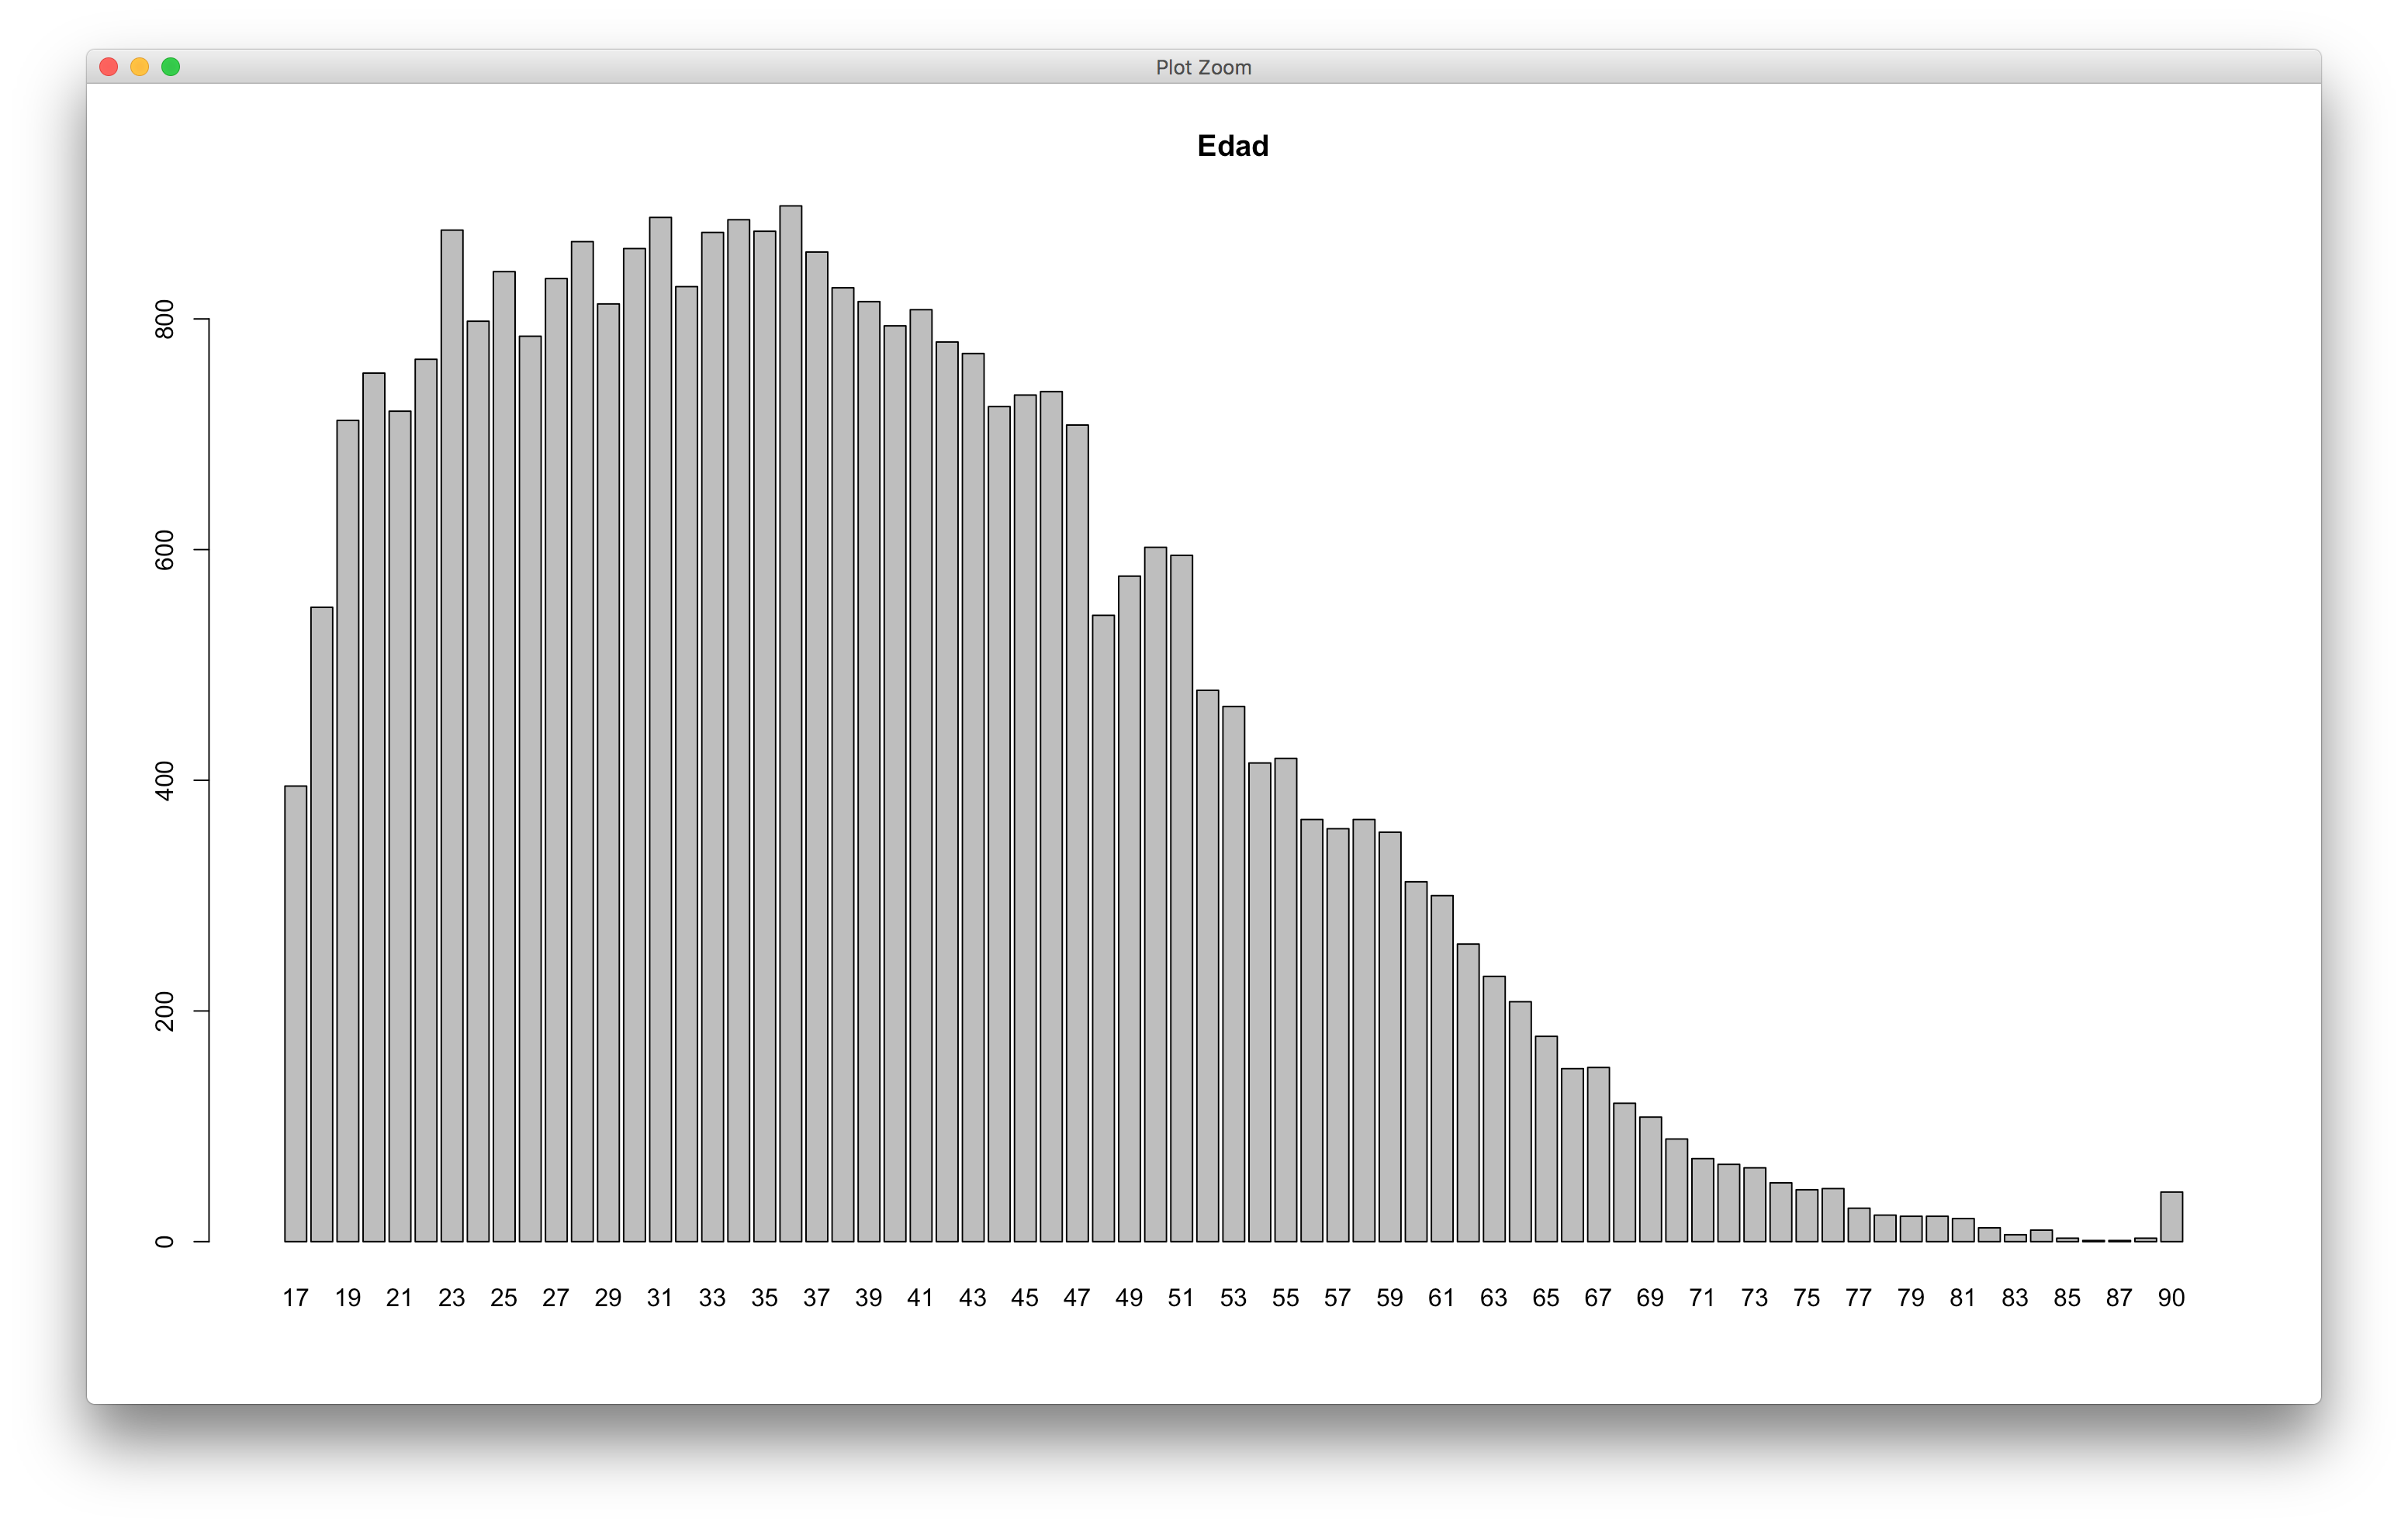
\includegraphics[scale=0.4]{graficas/edad}}
 \end{center}
 \begin{center}
   \hbox{\hspace{-5.8em}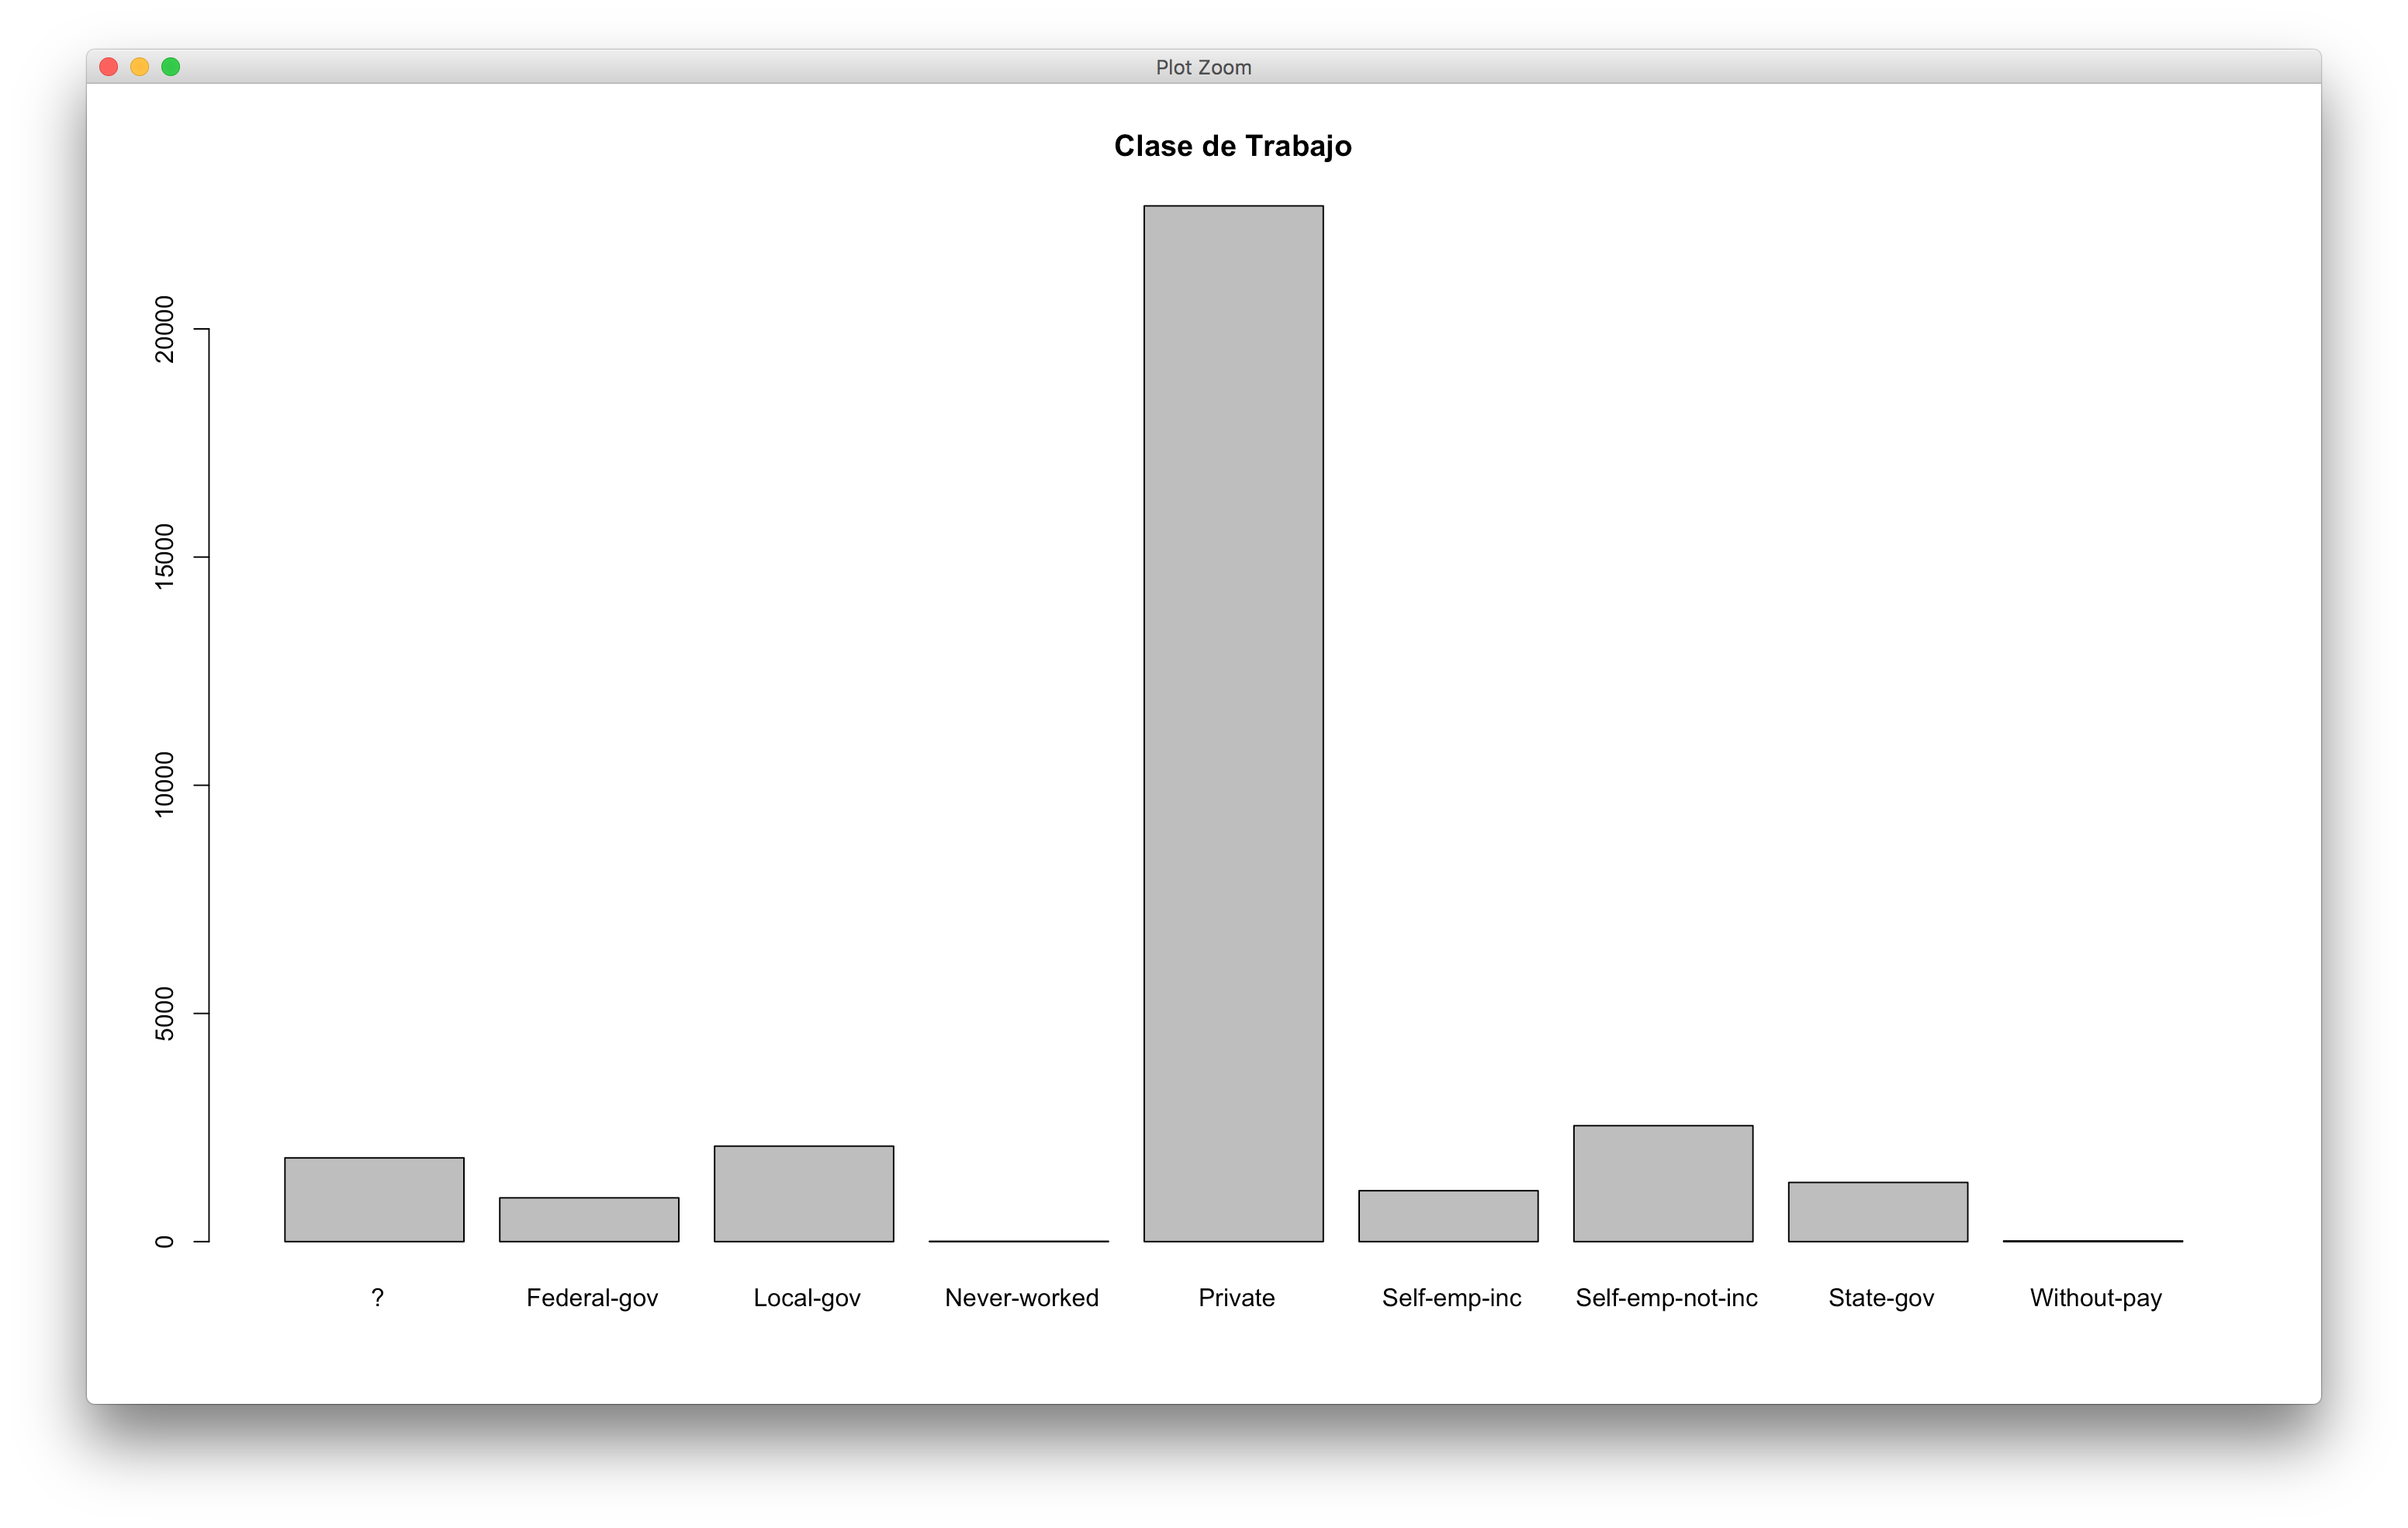
\includegraphics[scale=0.4]{graficas/claseDeTrabajo}}
 \end{center}
 \begin{center}
   \hbox{\hspace{-5.8em}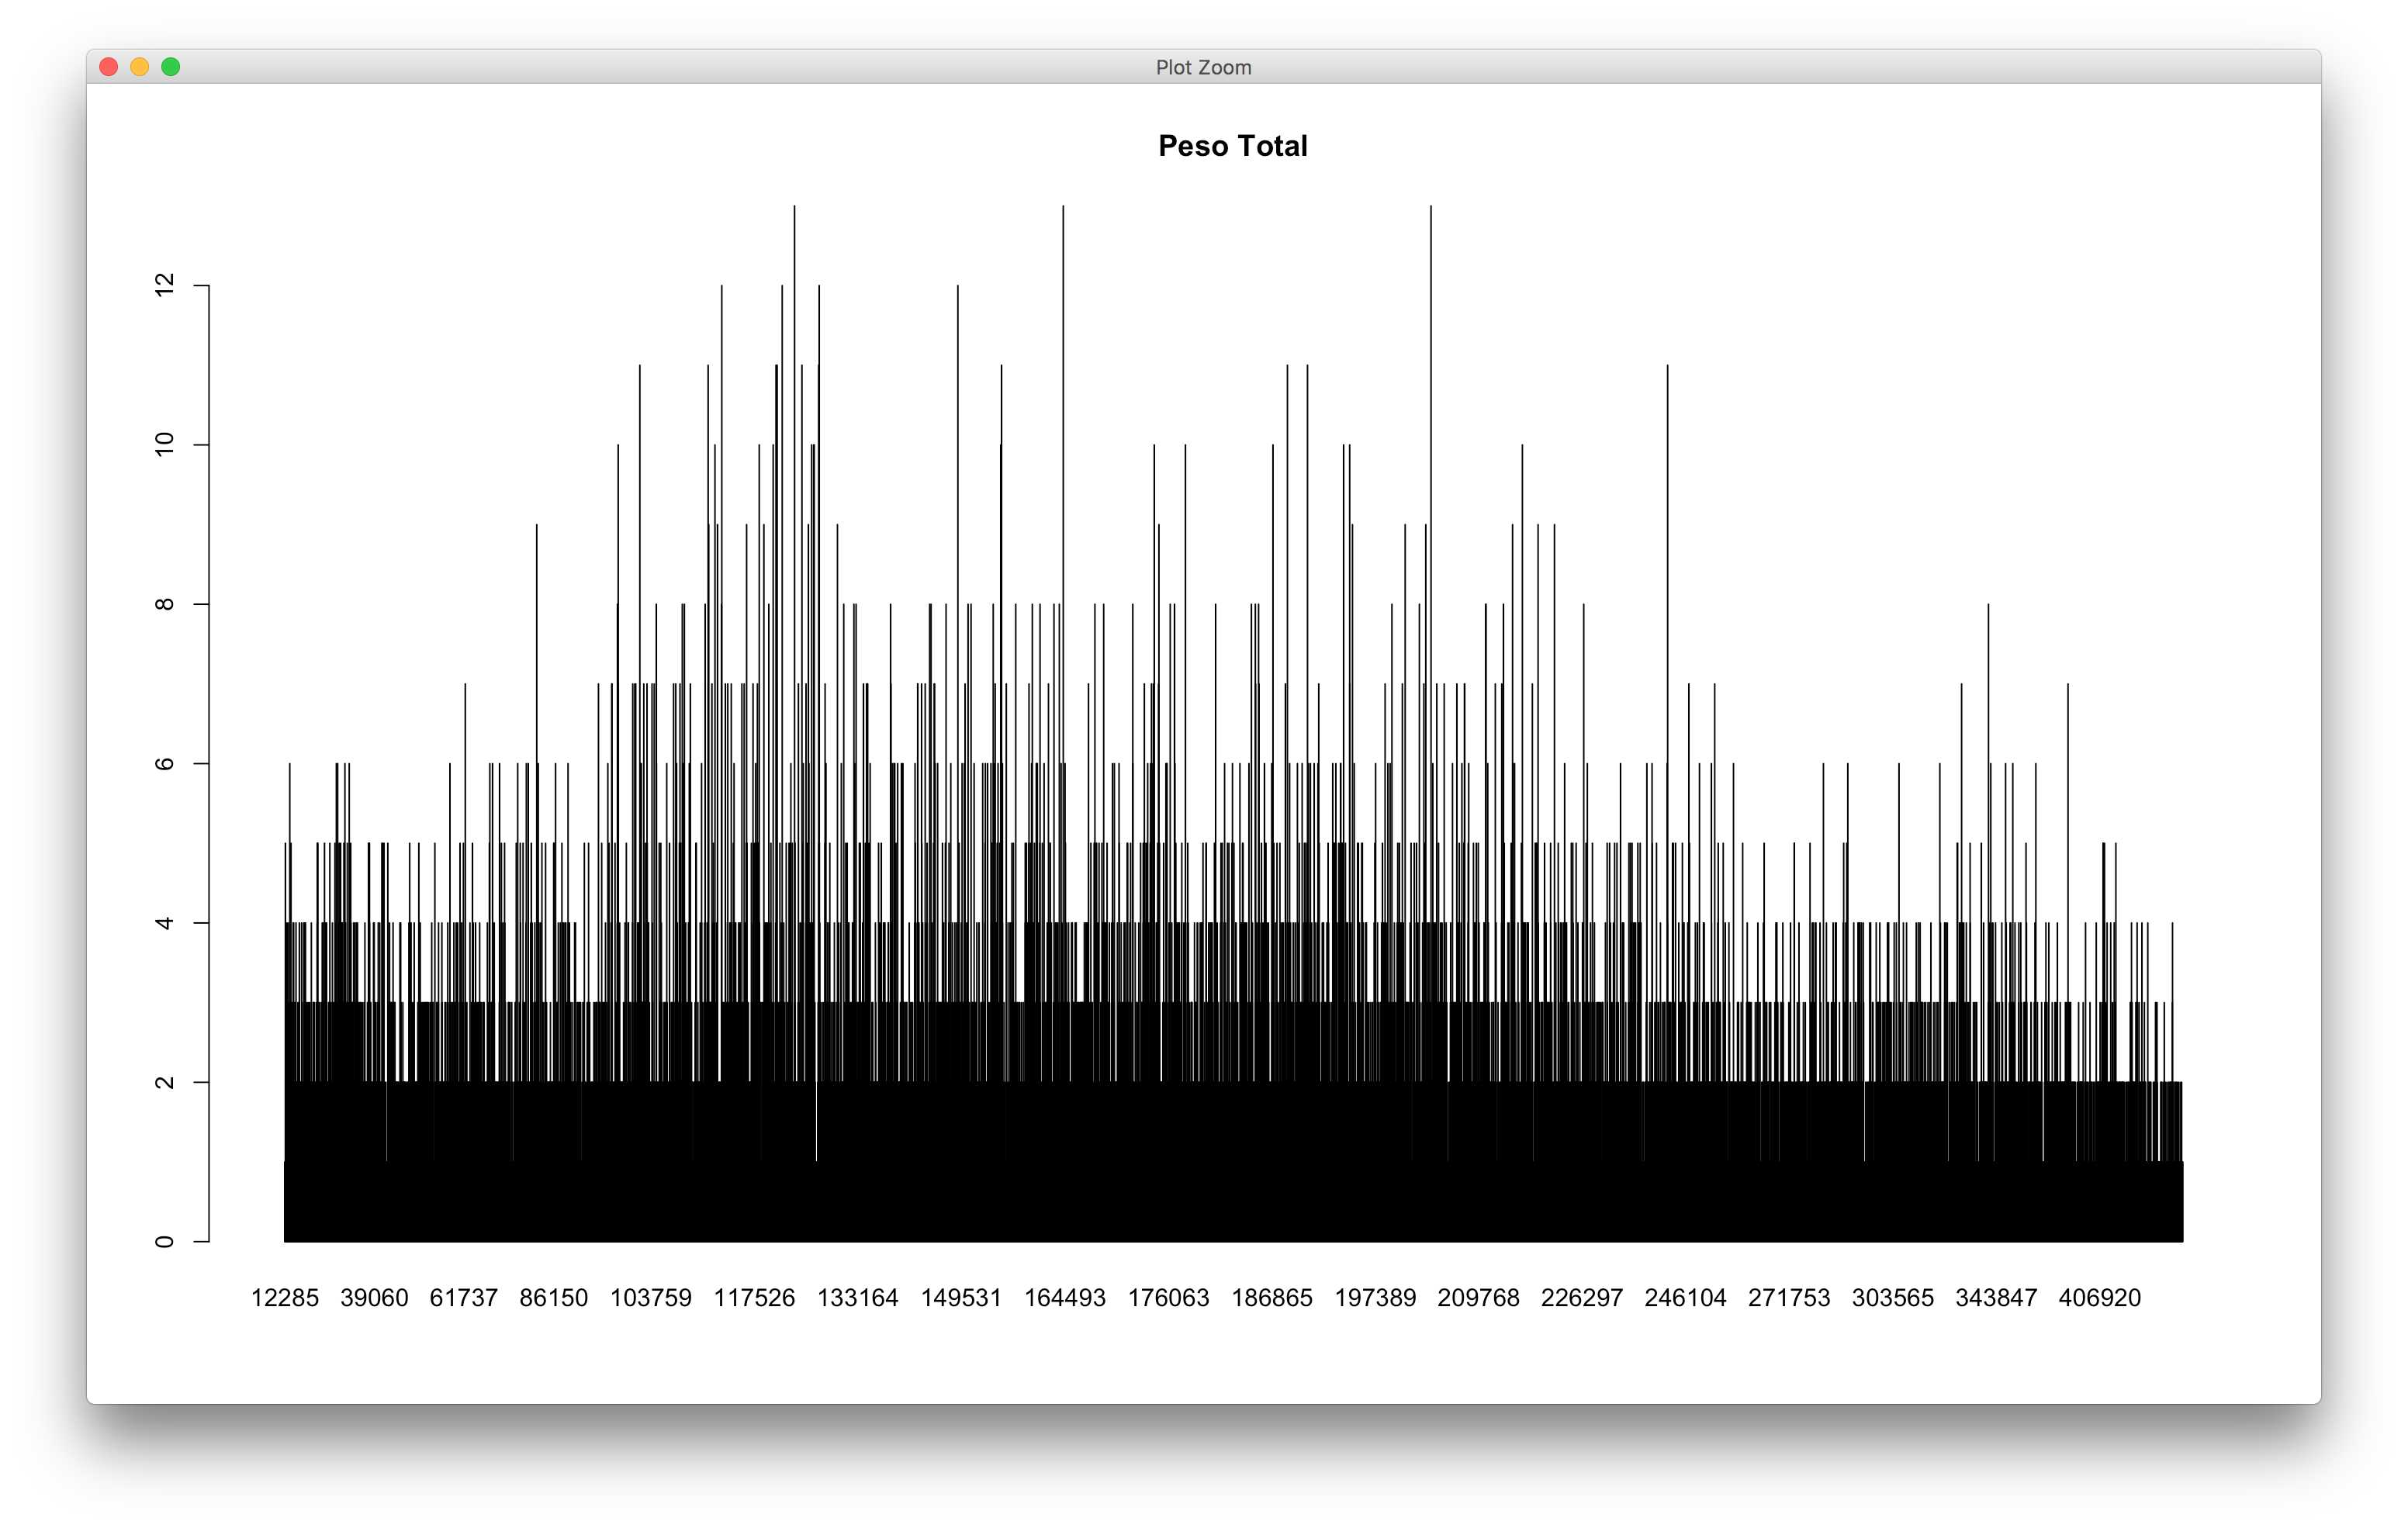
\includegraphics[scale=0.4]{graficas/pesoTotal}}
 \end{center}
 \begin{center}
   \hbox{\hspace{-5.8em}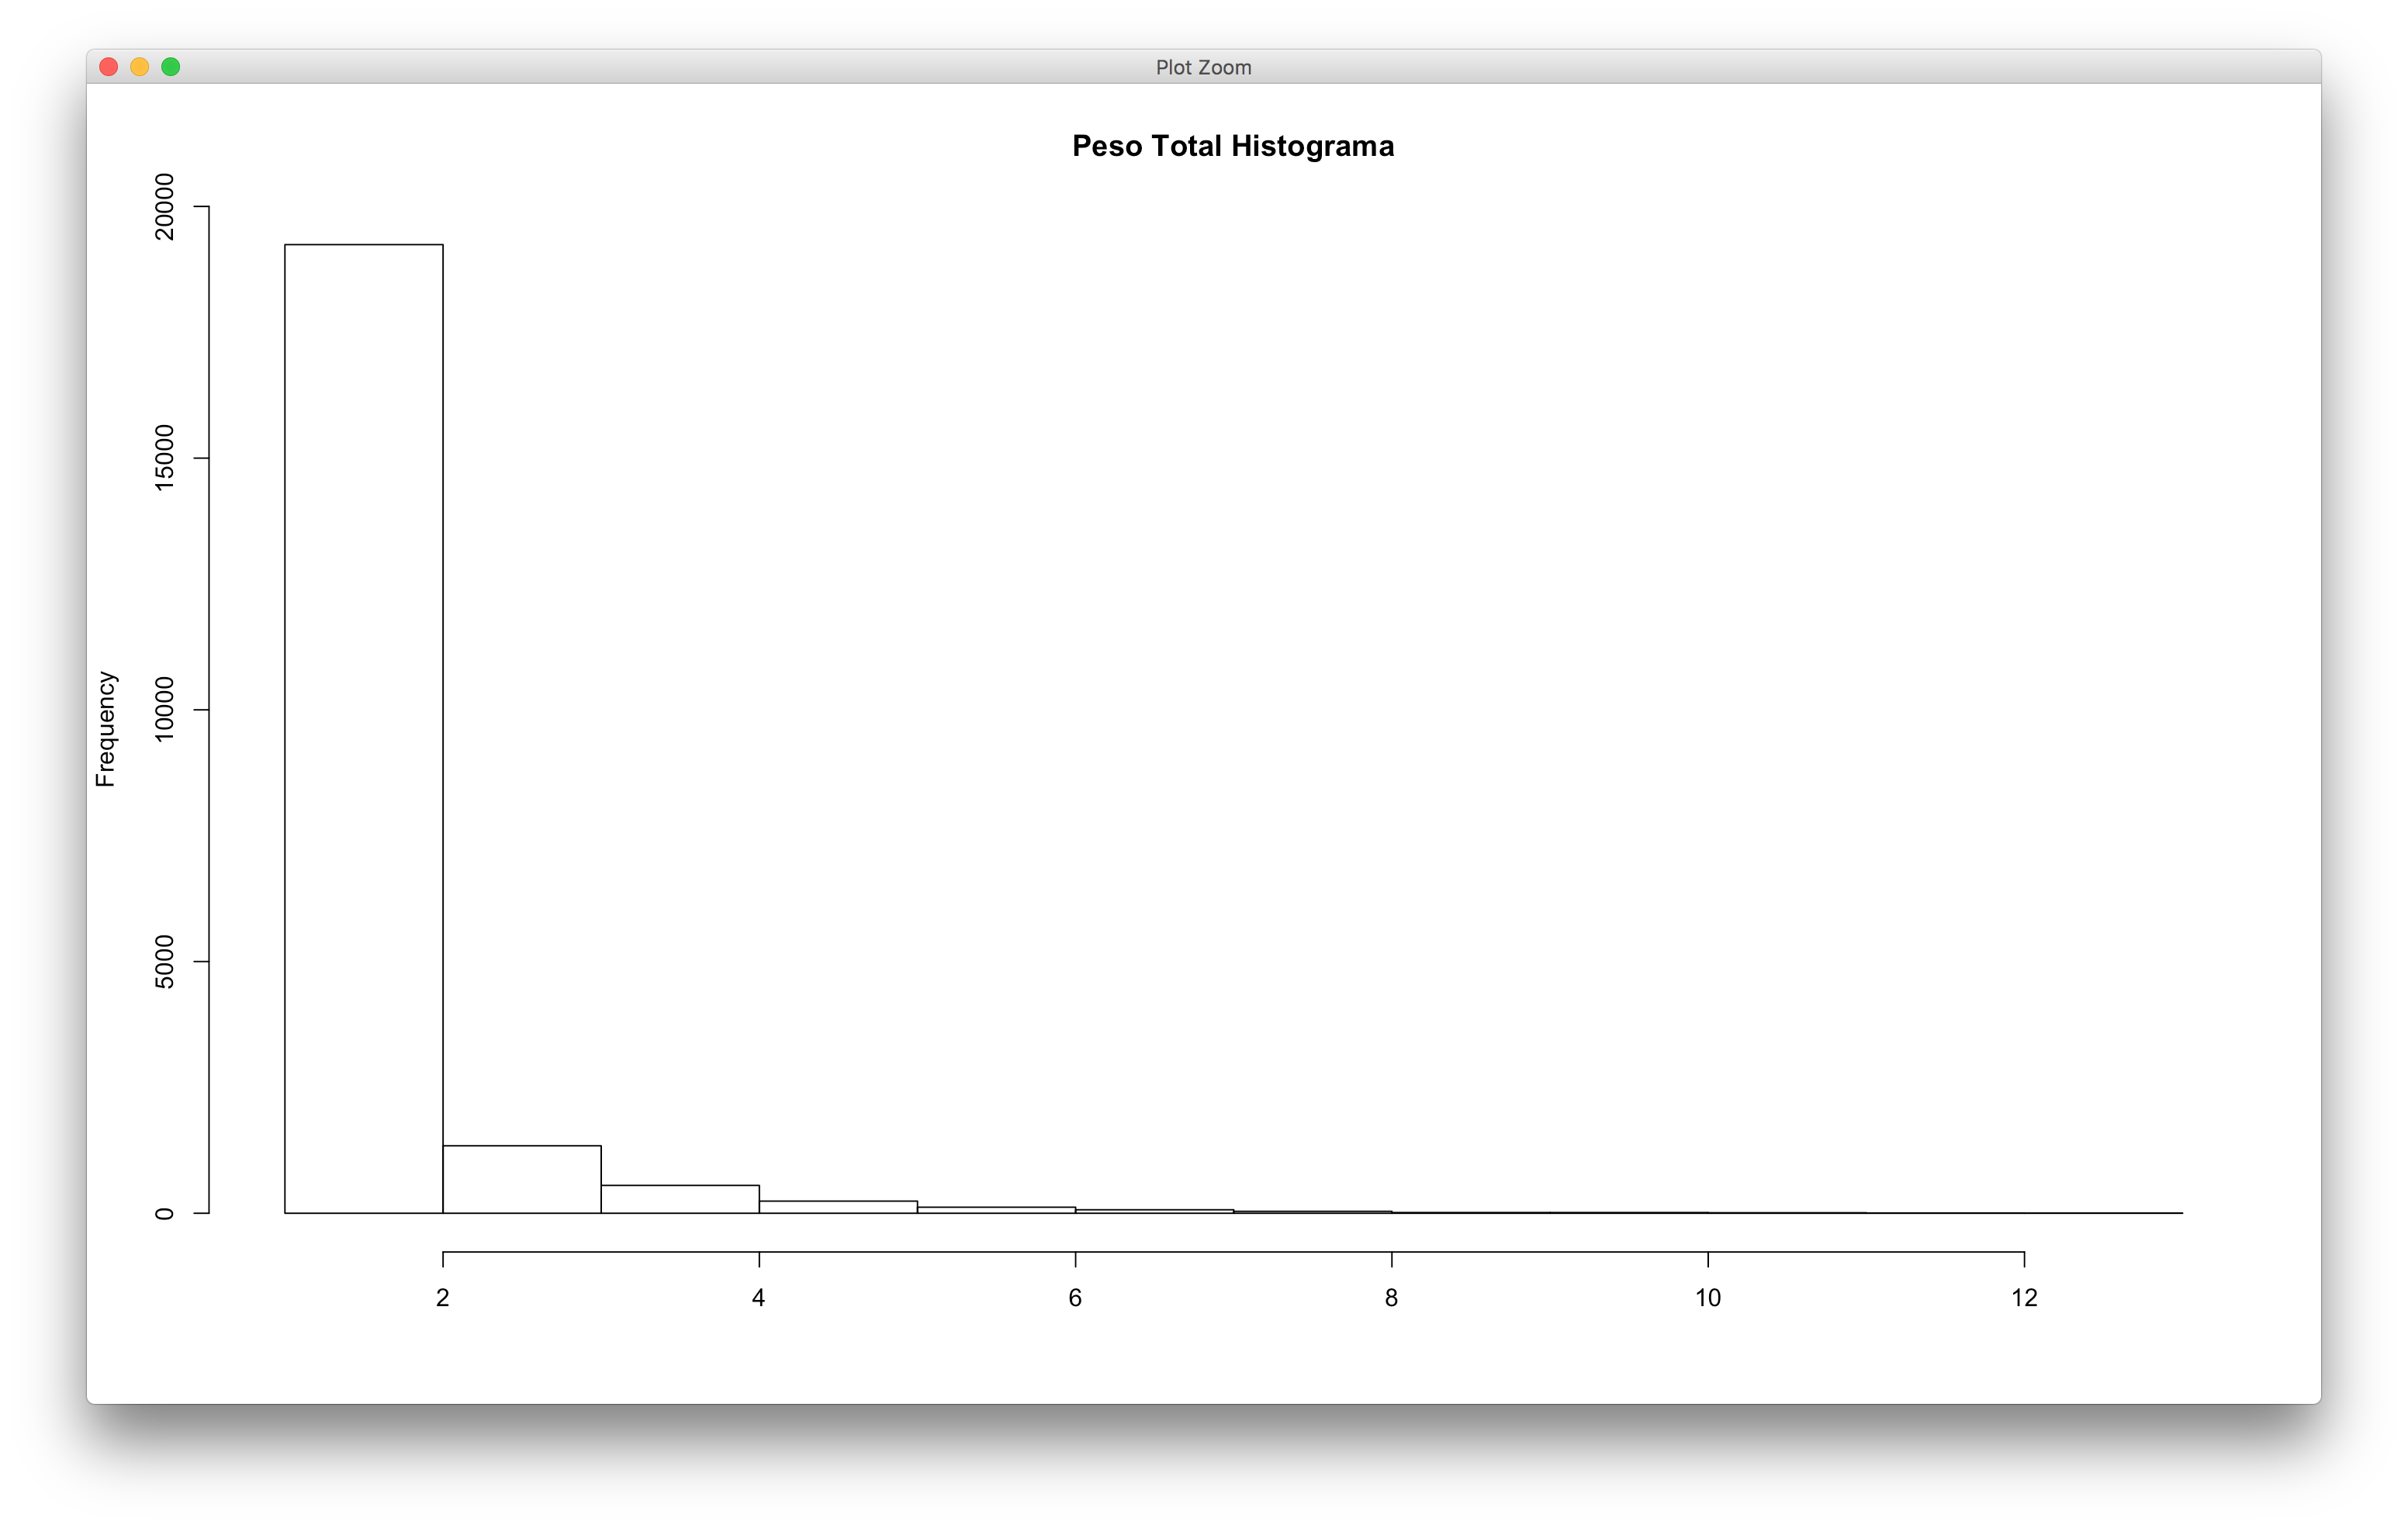
\includegraphics[scale=0.4]{graficas/pesoTotalHist}}
 \end{center}
 \begin{center}
   \hbox{\hspace{-6.1em}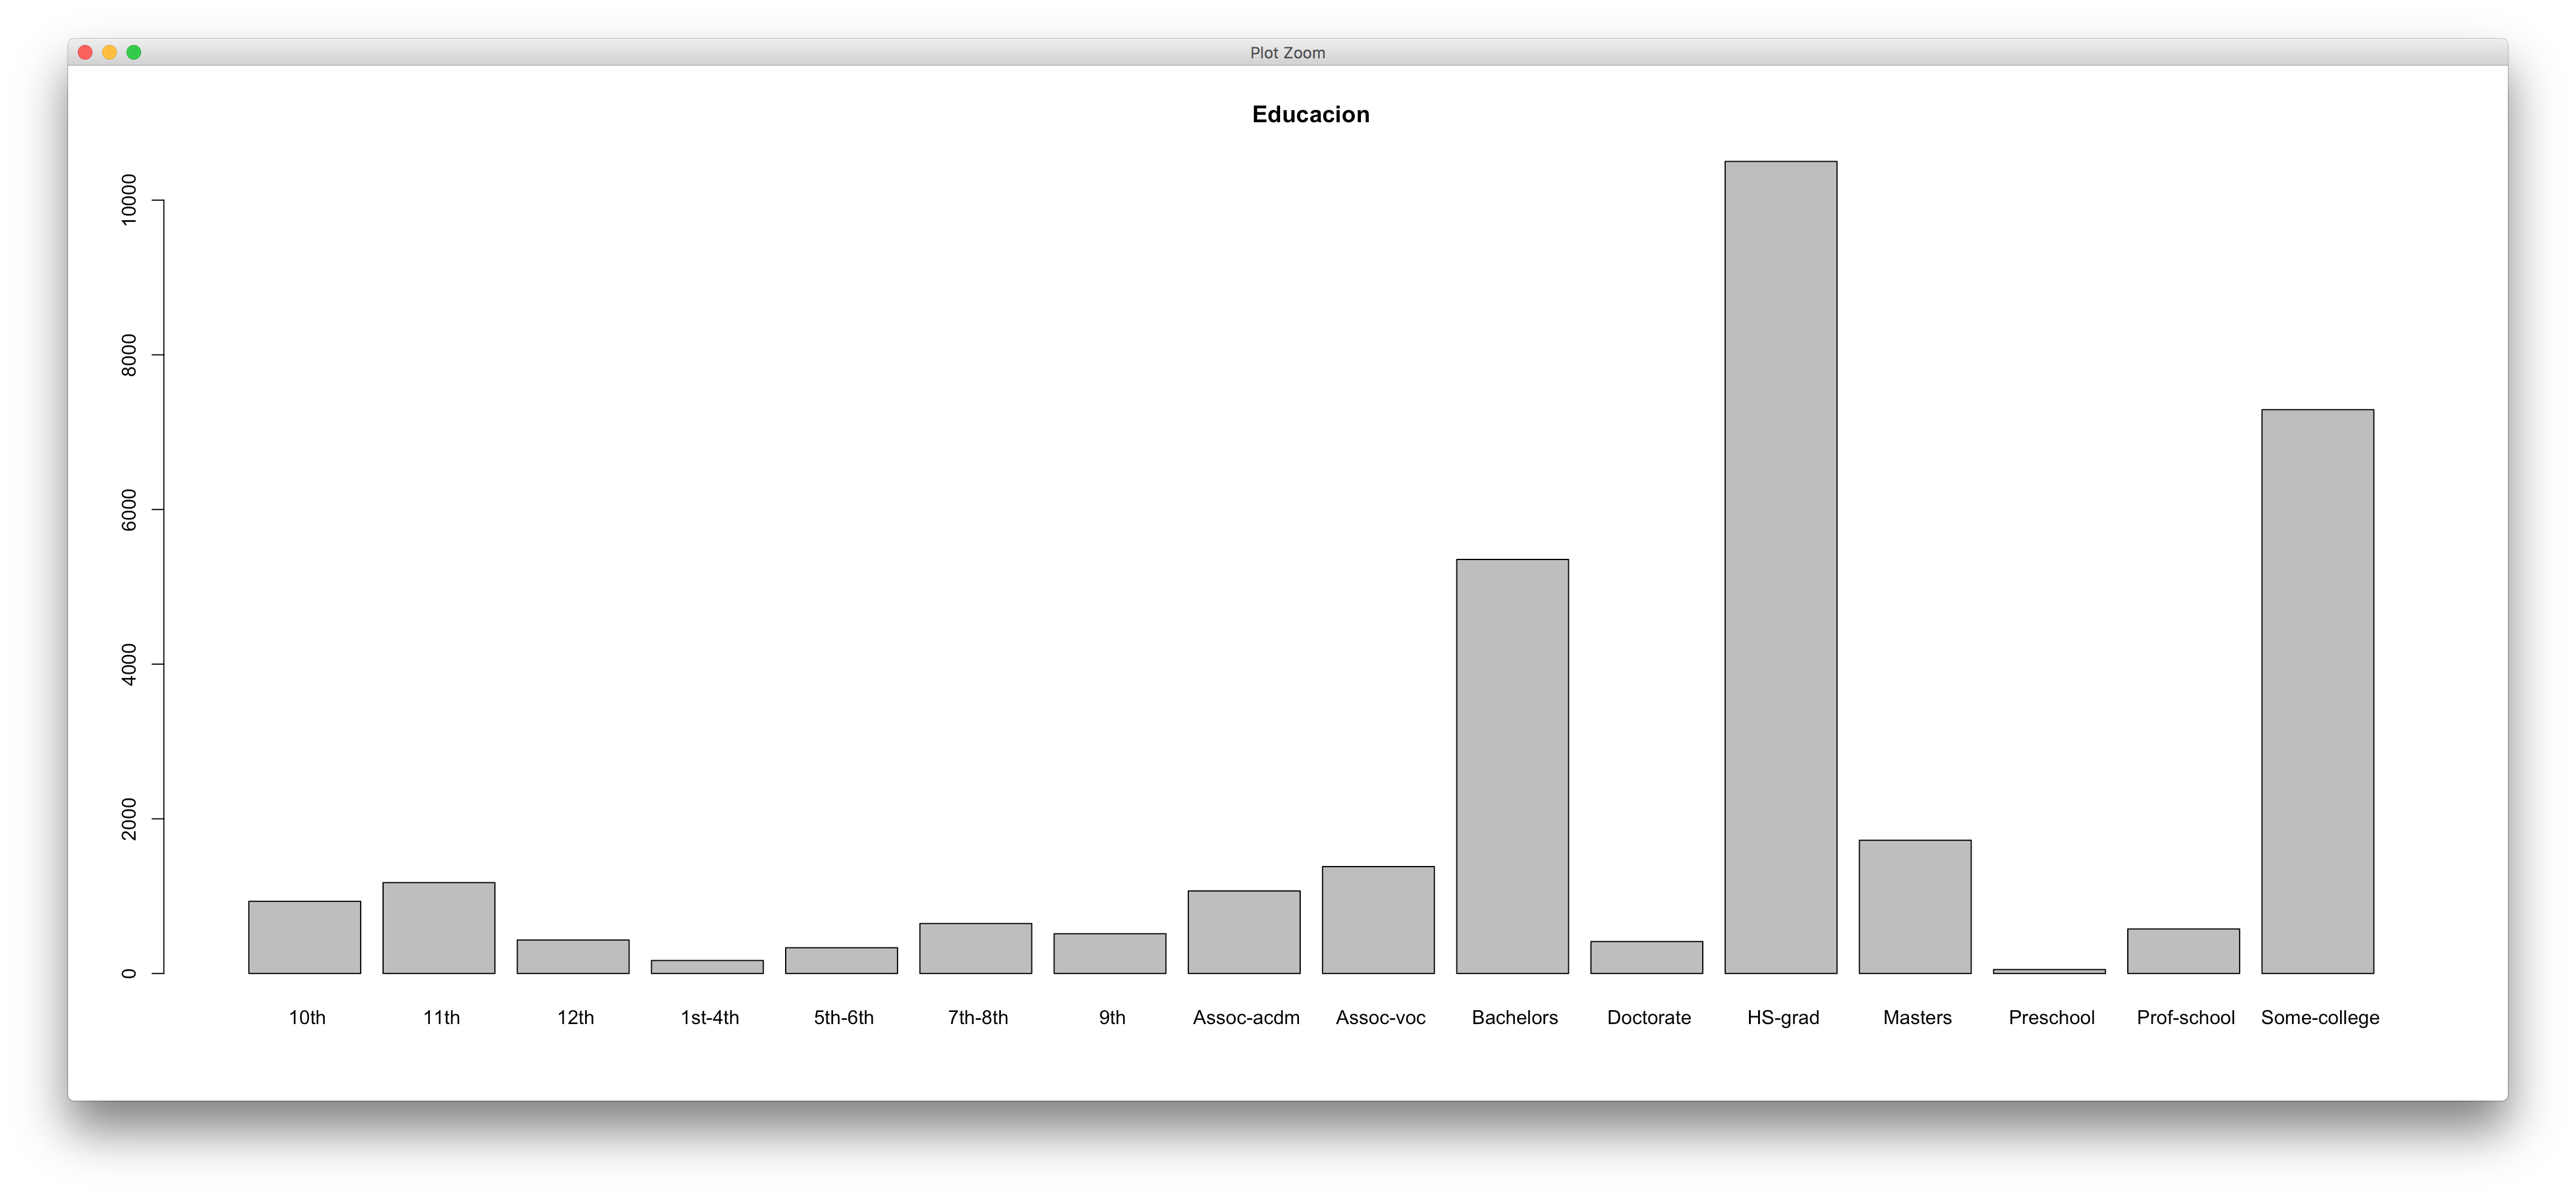
\includegraphics[scale=0.3]{graficas/educacion}}
 \end{center}
 \begin{center}
   \hbox{\hspace{-5.8em}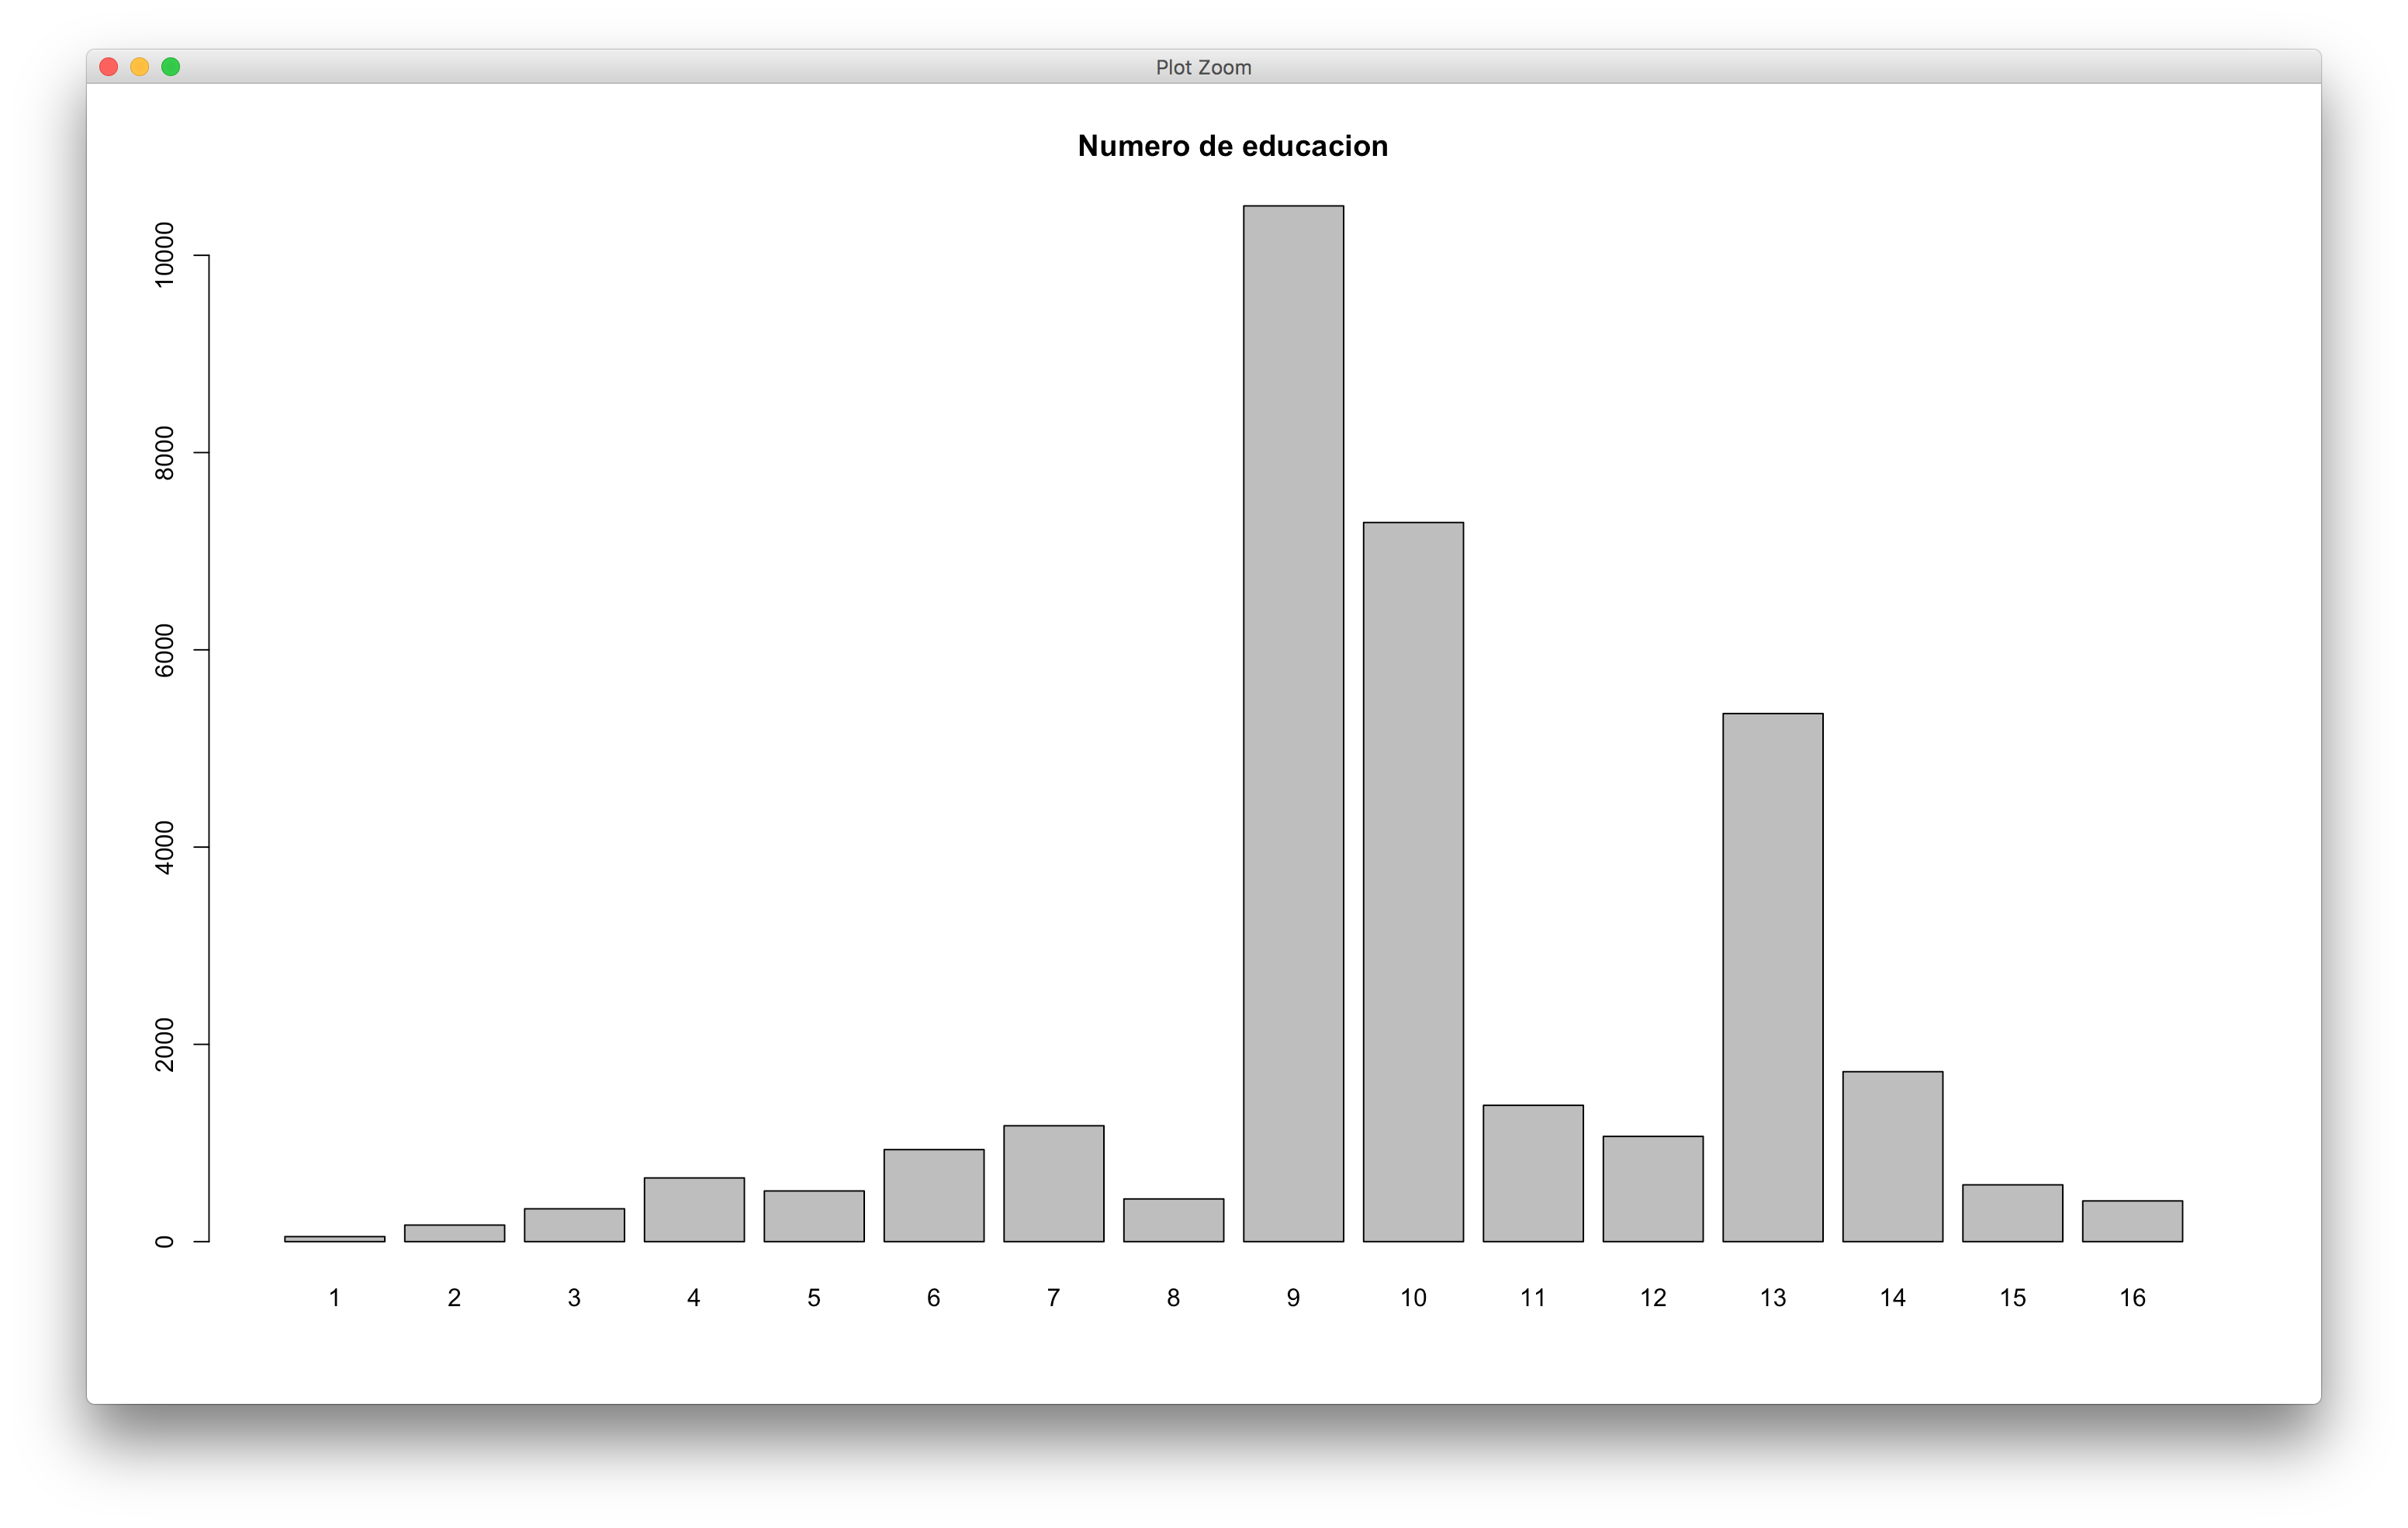
\includegraphics[scale=0.4]{graficas/numeroDeEducacion}}
 \end{center}
 \begin{center}
   \hbox{\hspace{-5.8em}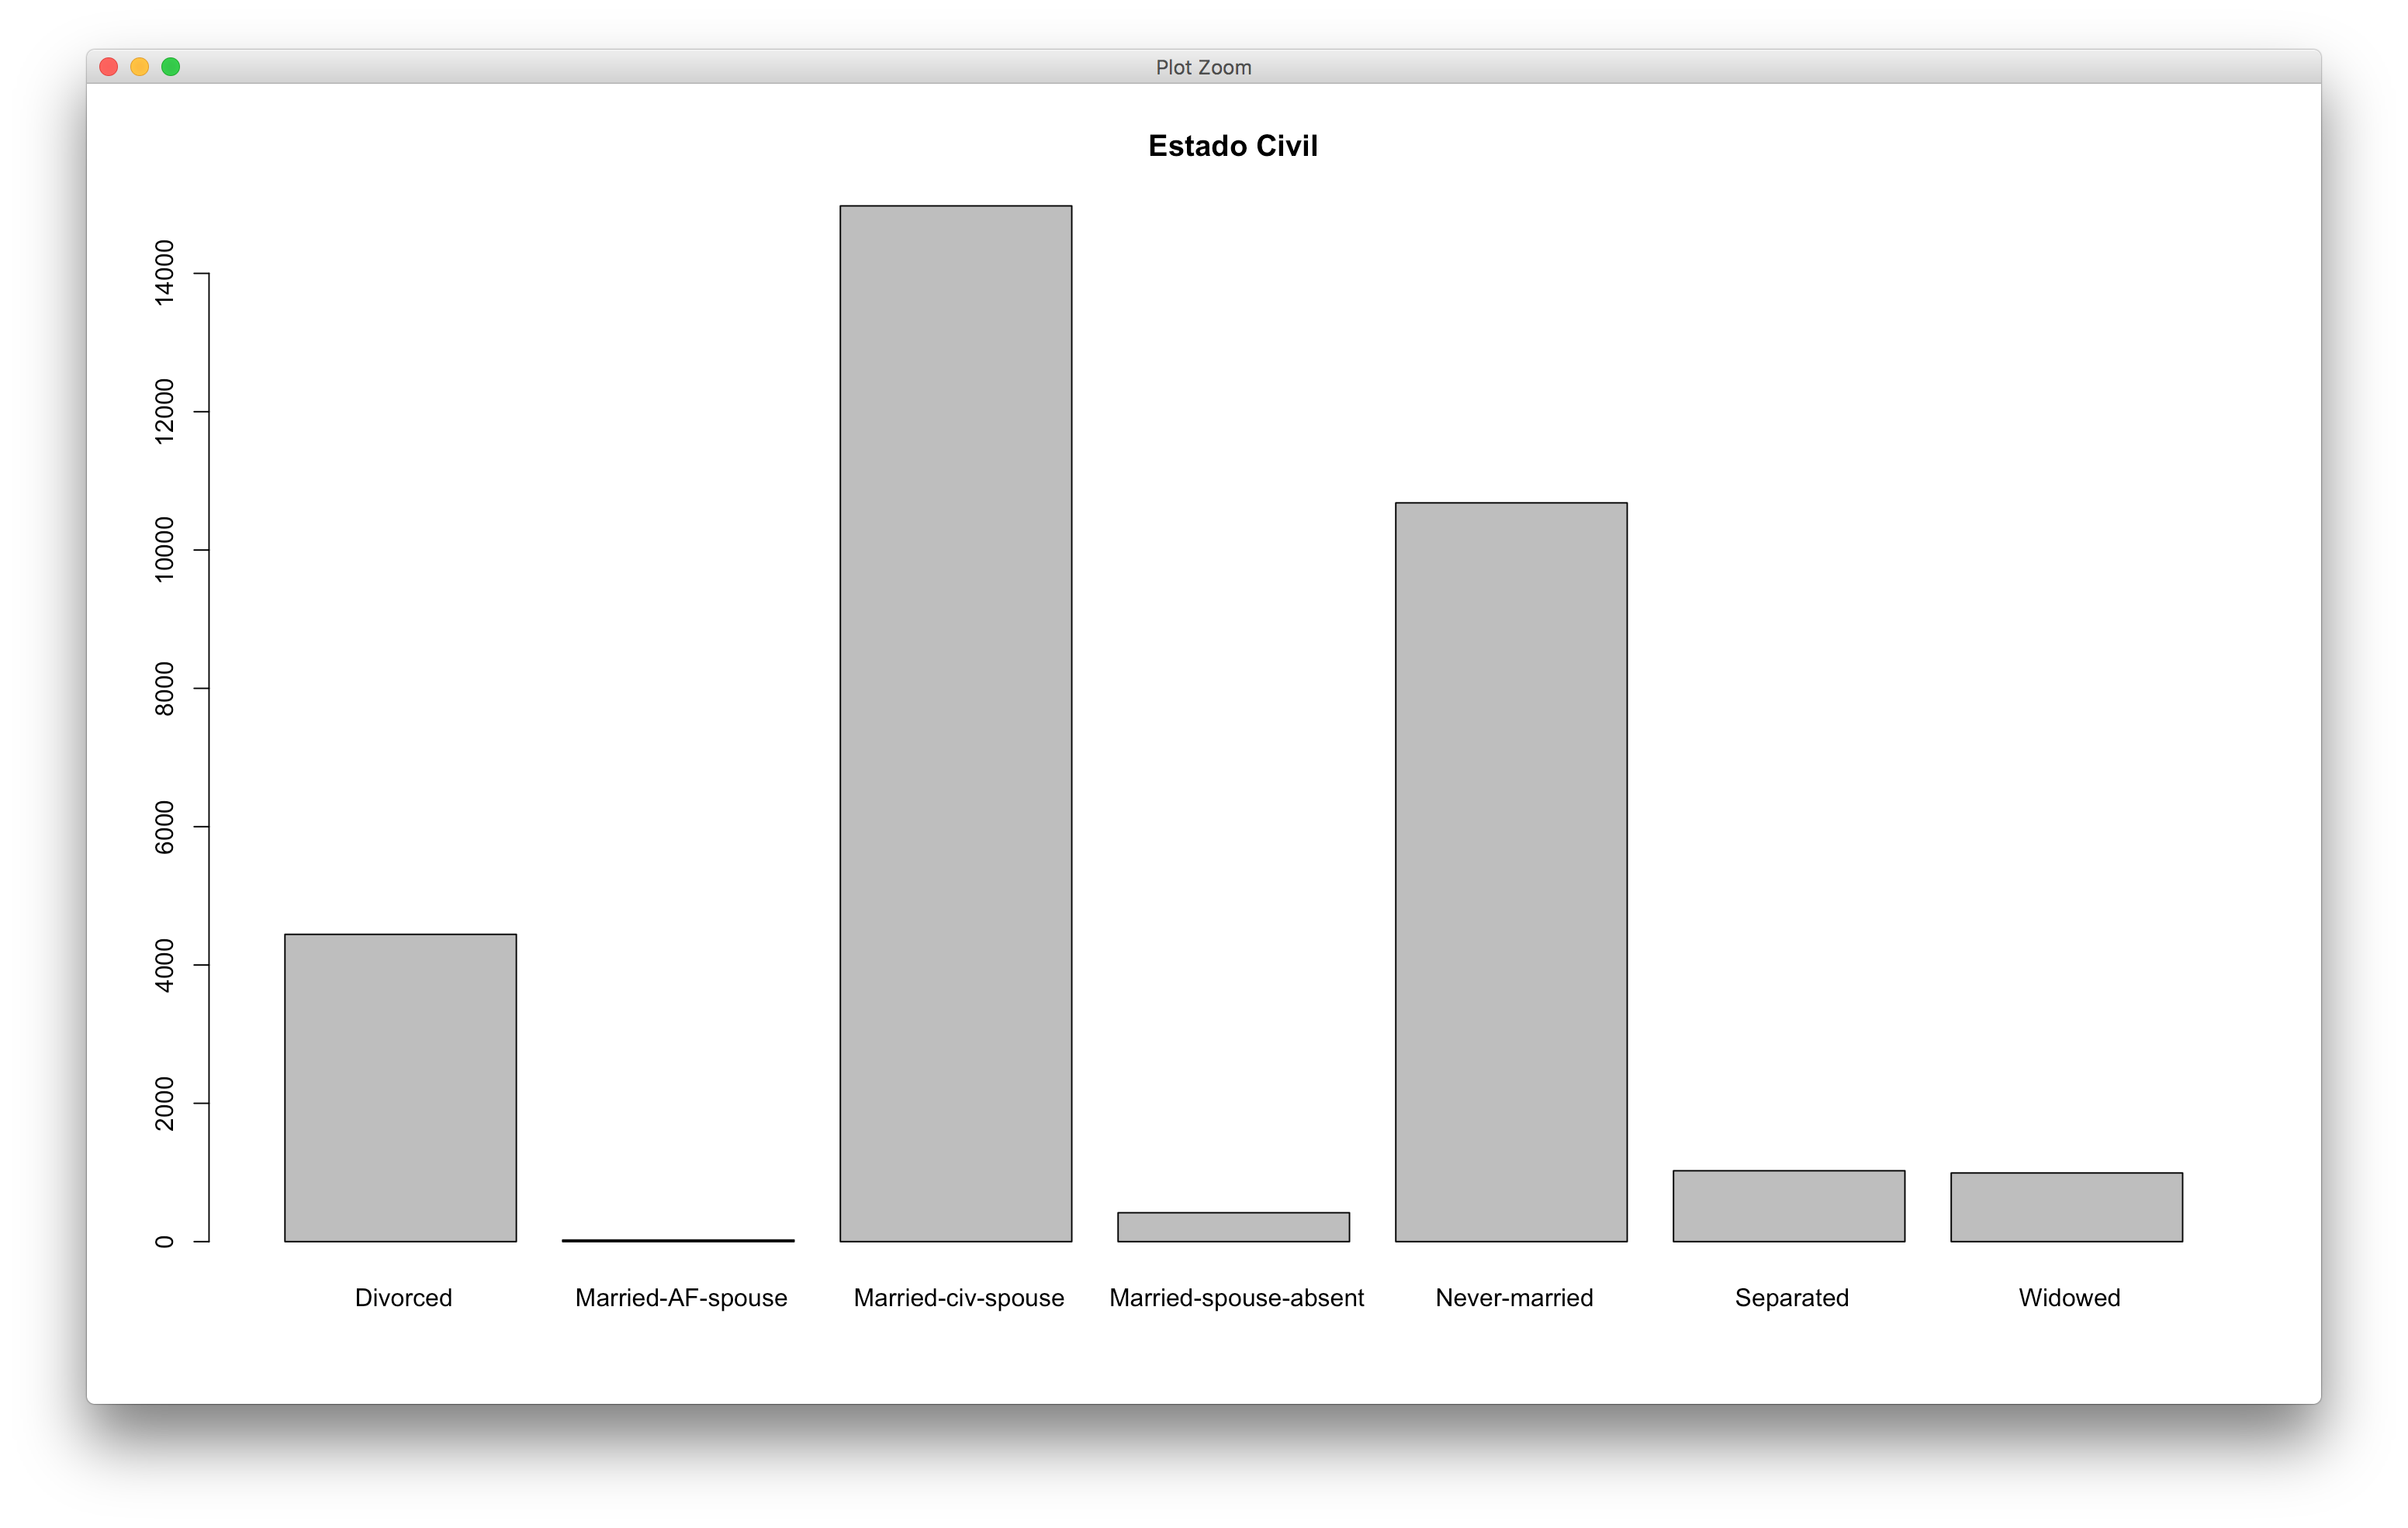
\includegraphics[scale=0.4]{graficas/EstadoCivil}}
 \end{center}
 \begin{center}
   \hbox{\hspace{-5.8em}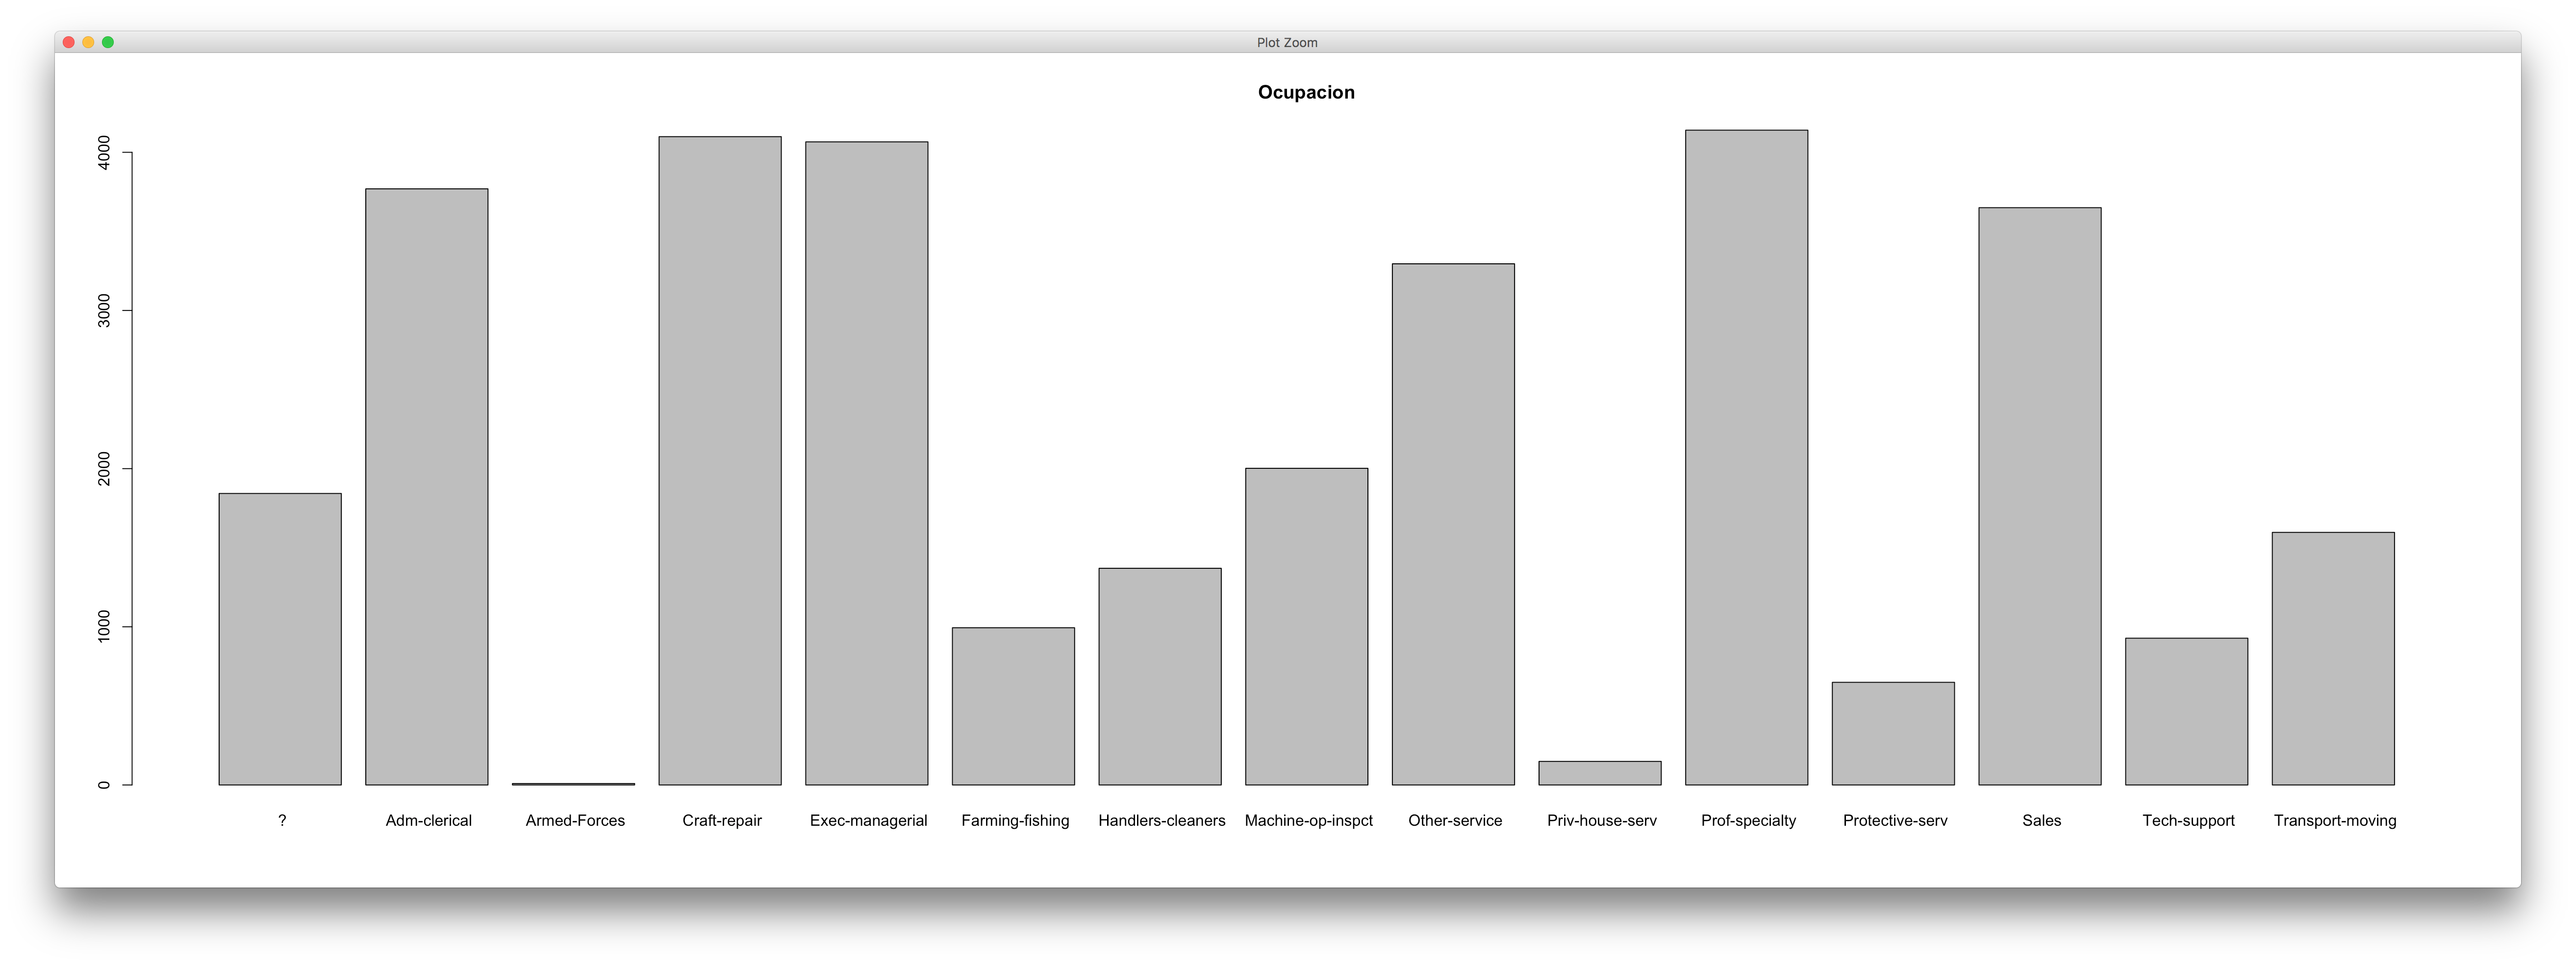
\includegraphics[scale=0.23]{graficas/ocupacion}}
 \end{center}
 \begin{center}
   \hbox{\hspace{-5.8em}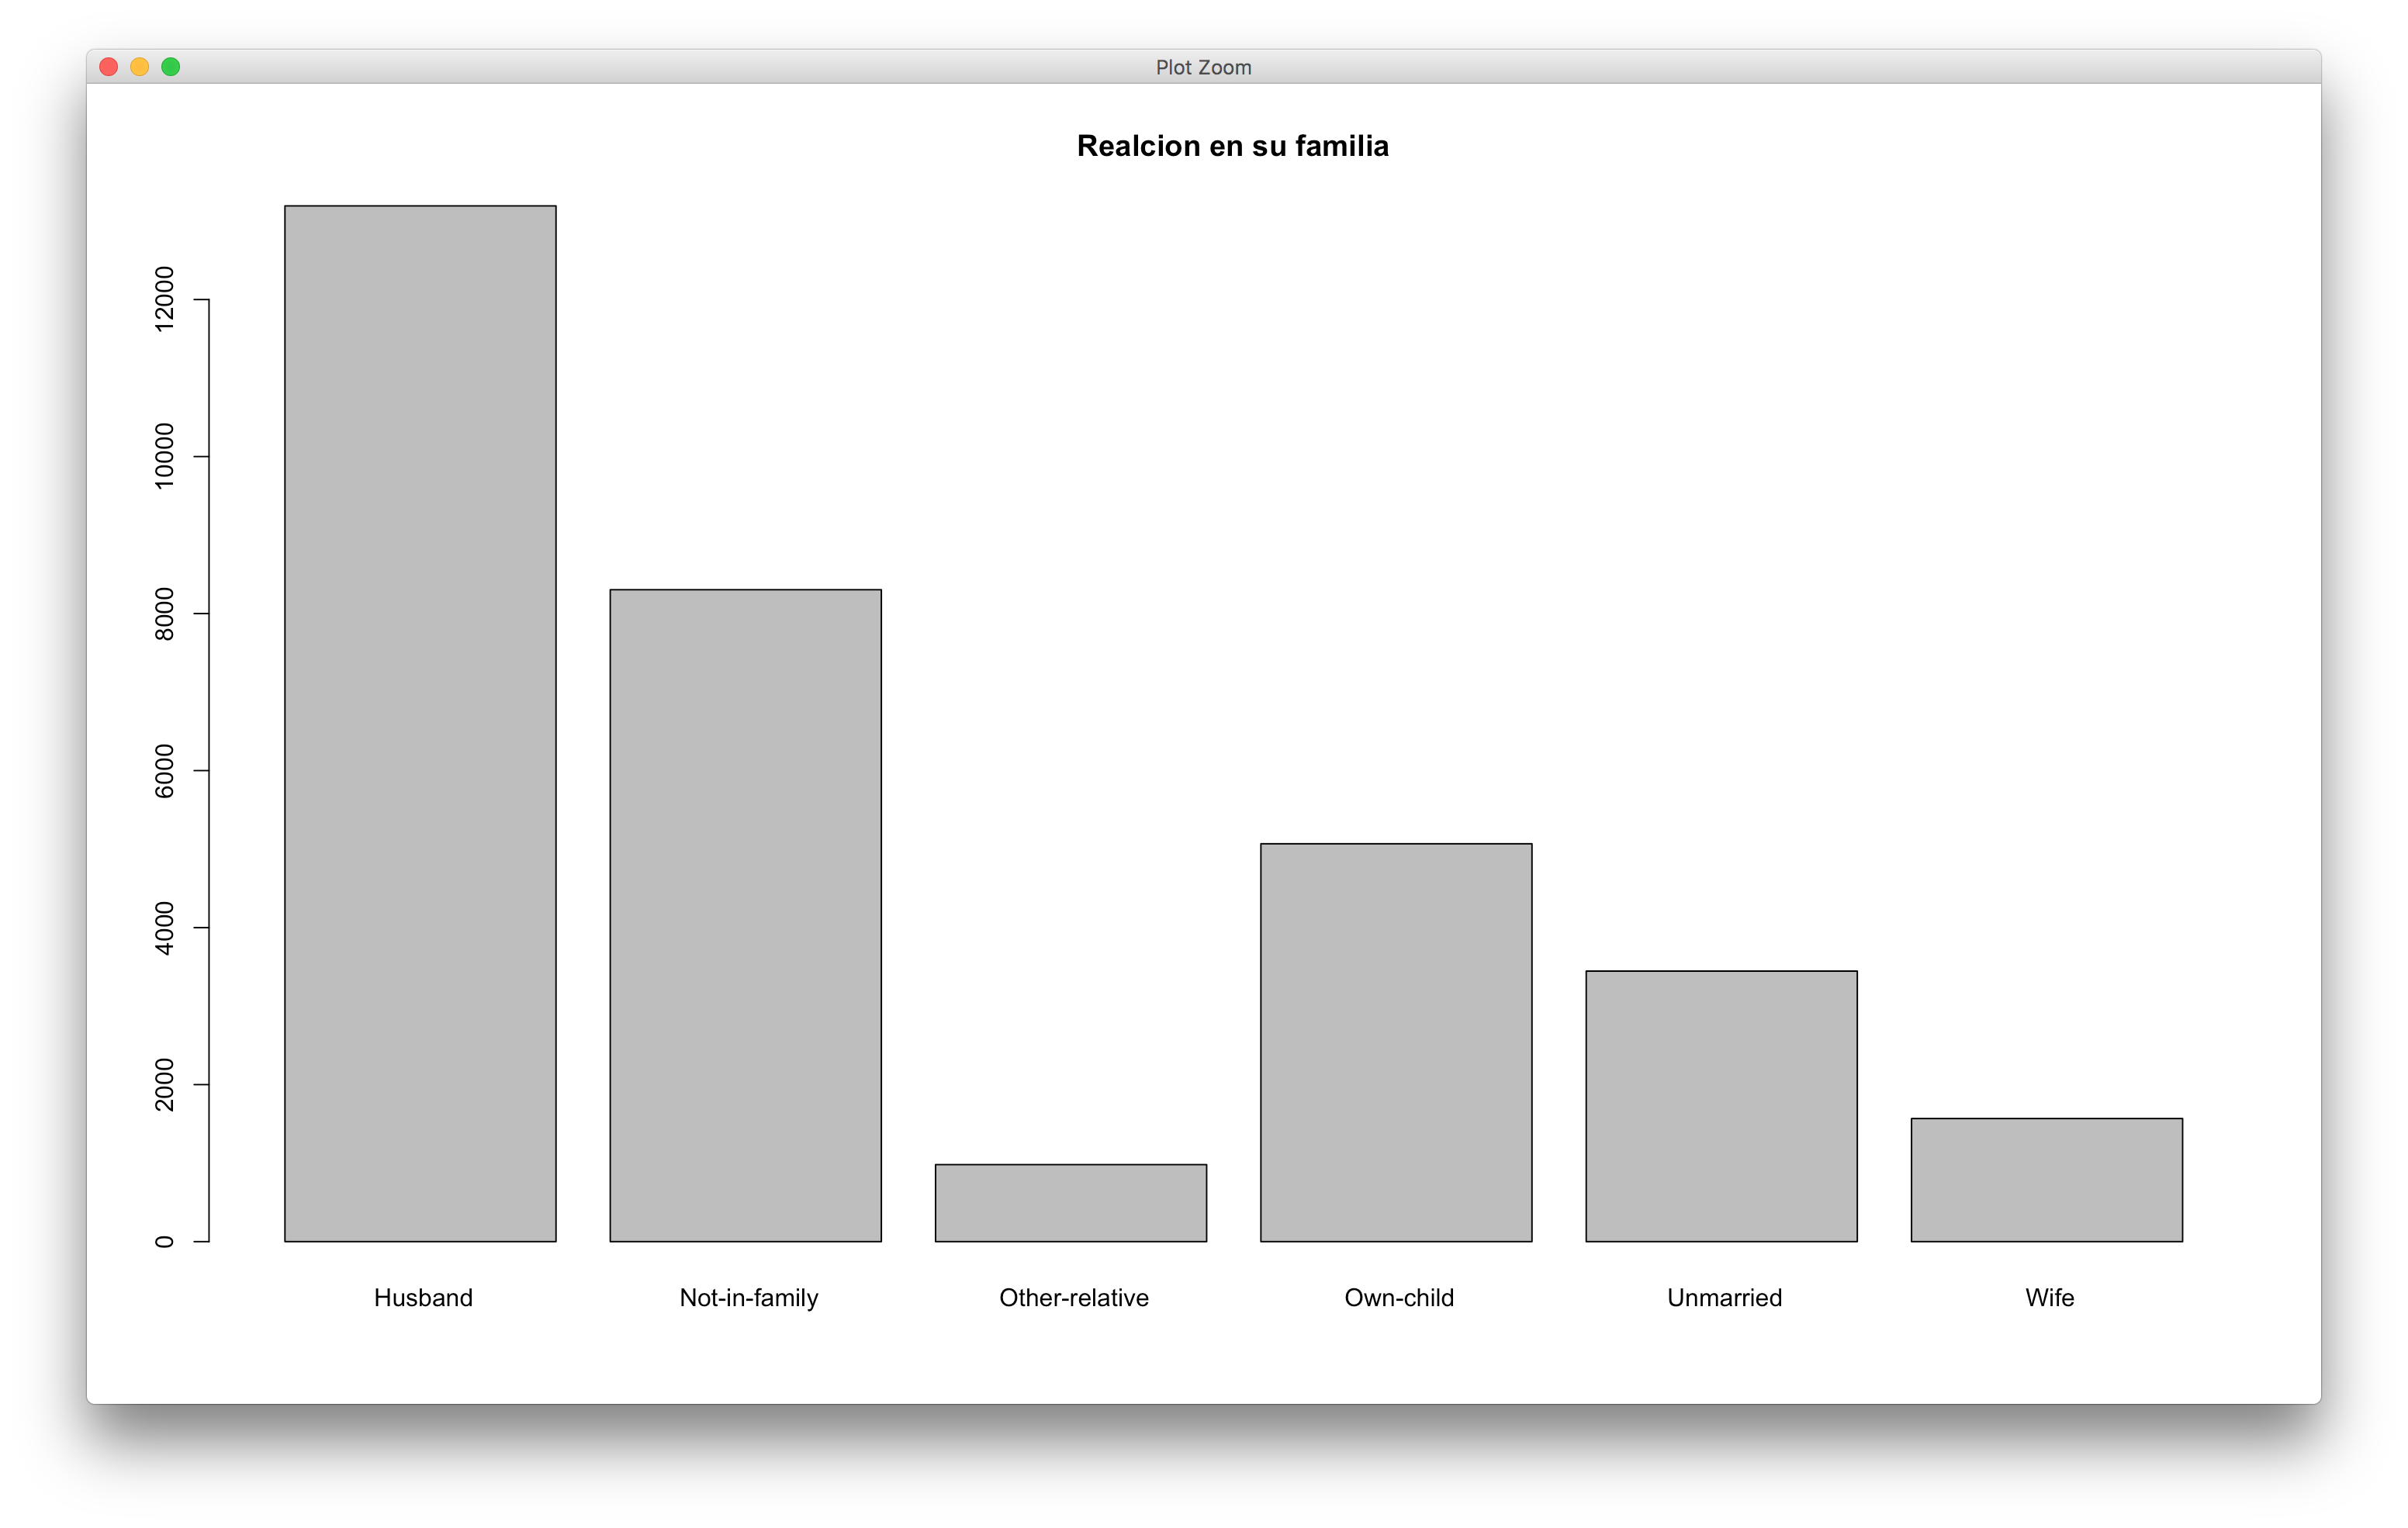
\includegraphics[scale=0.4]{graficas/relacionEnSuFamilia}}
 \end{center}
 \begin{center}
   \hbox{\hspace{-5.8em}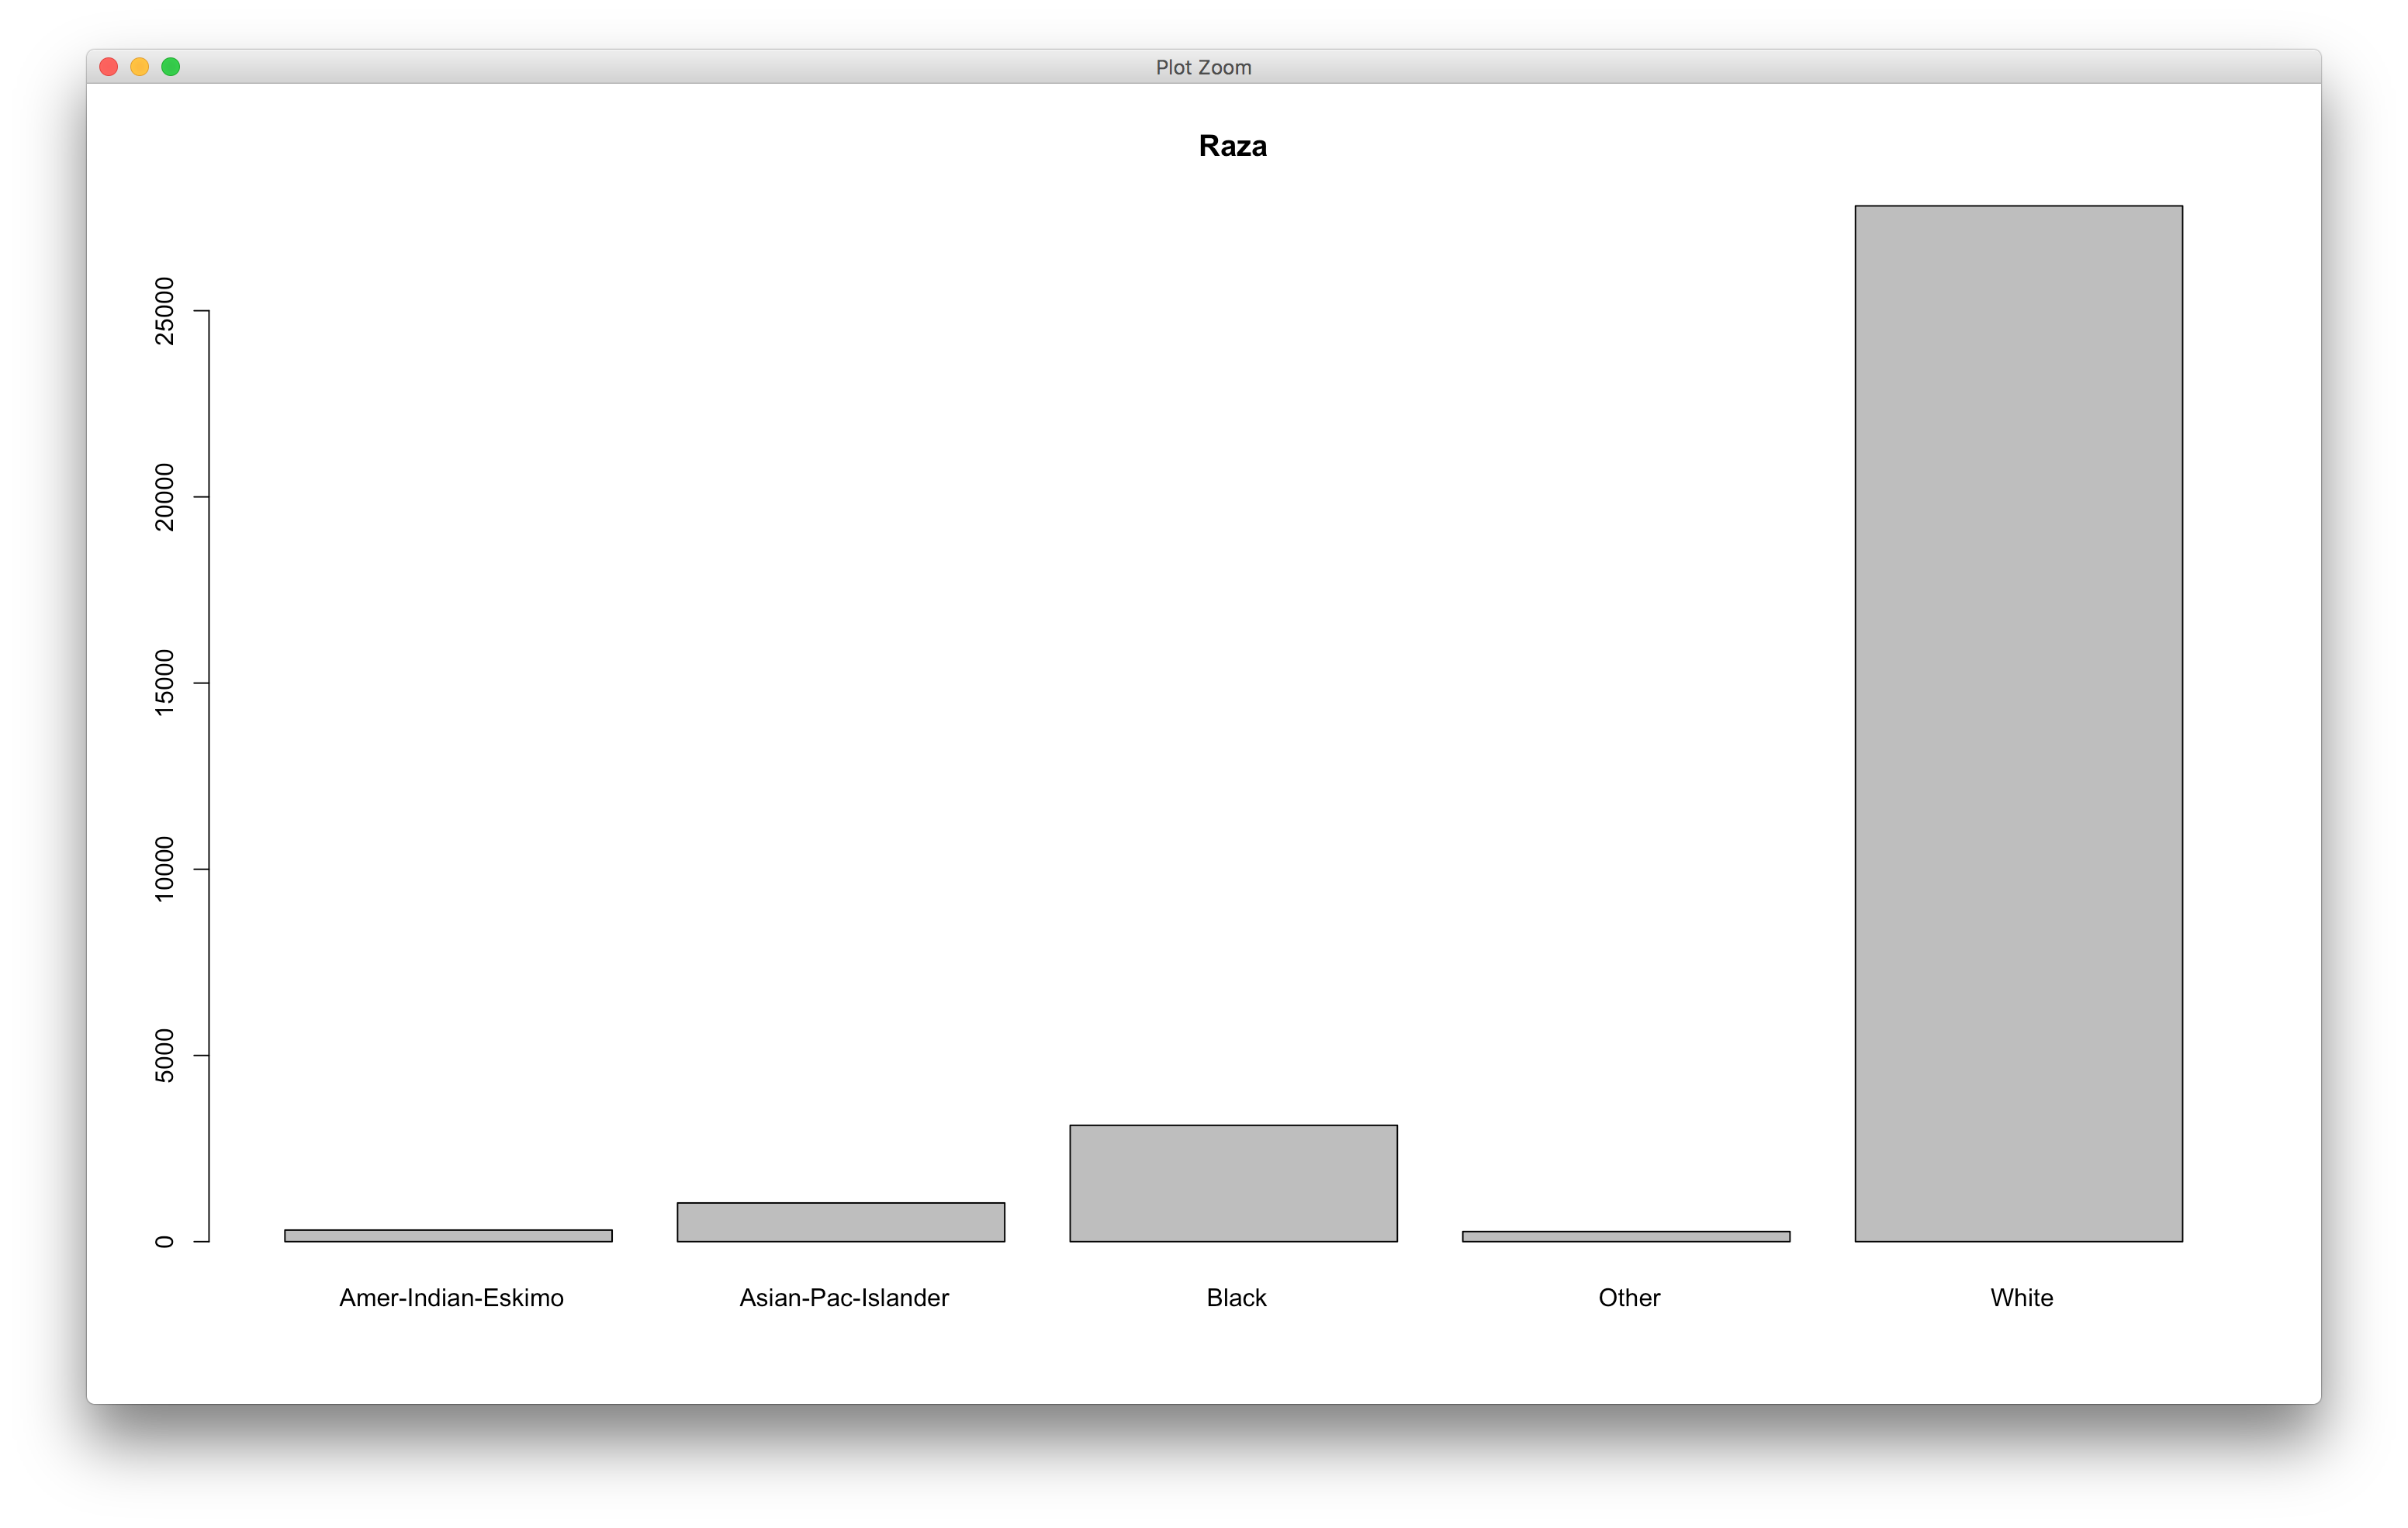
\includegraphics[scale=0.4]{graficas/raza}}
 \end{center}
 \begin{center}
   \hbox{\hspace{-5.8em}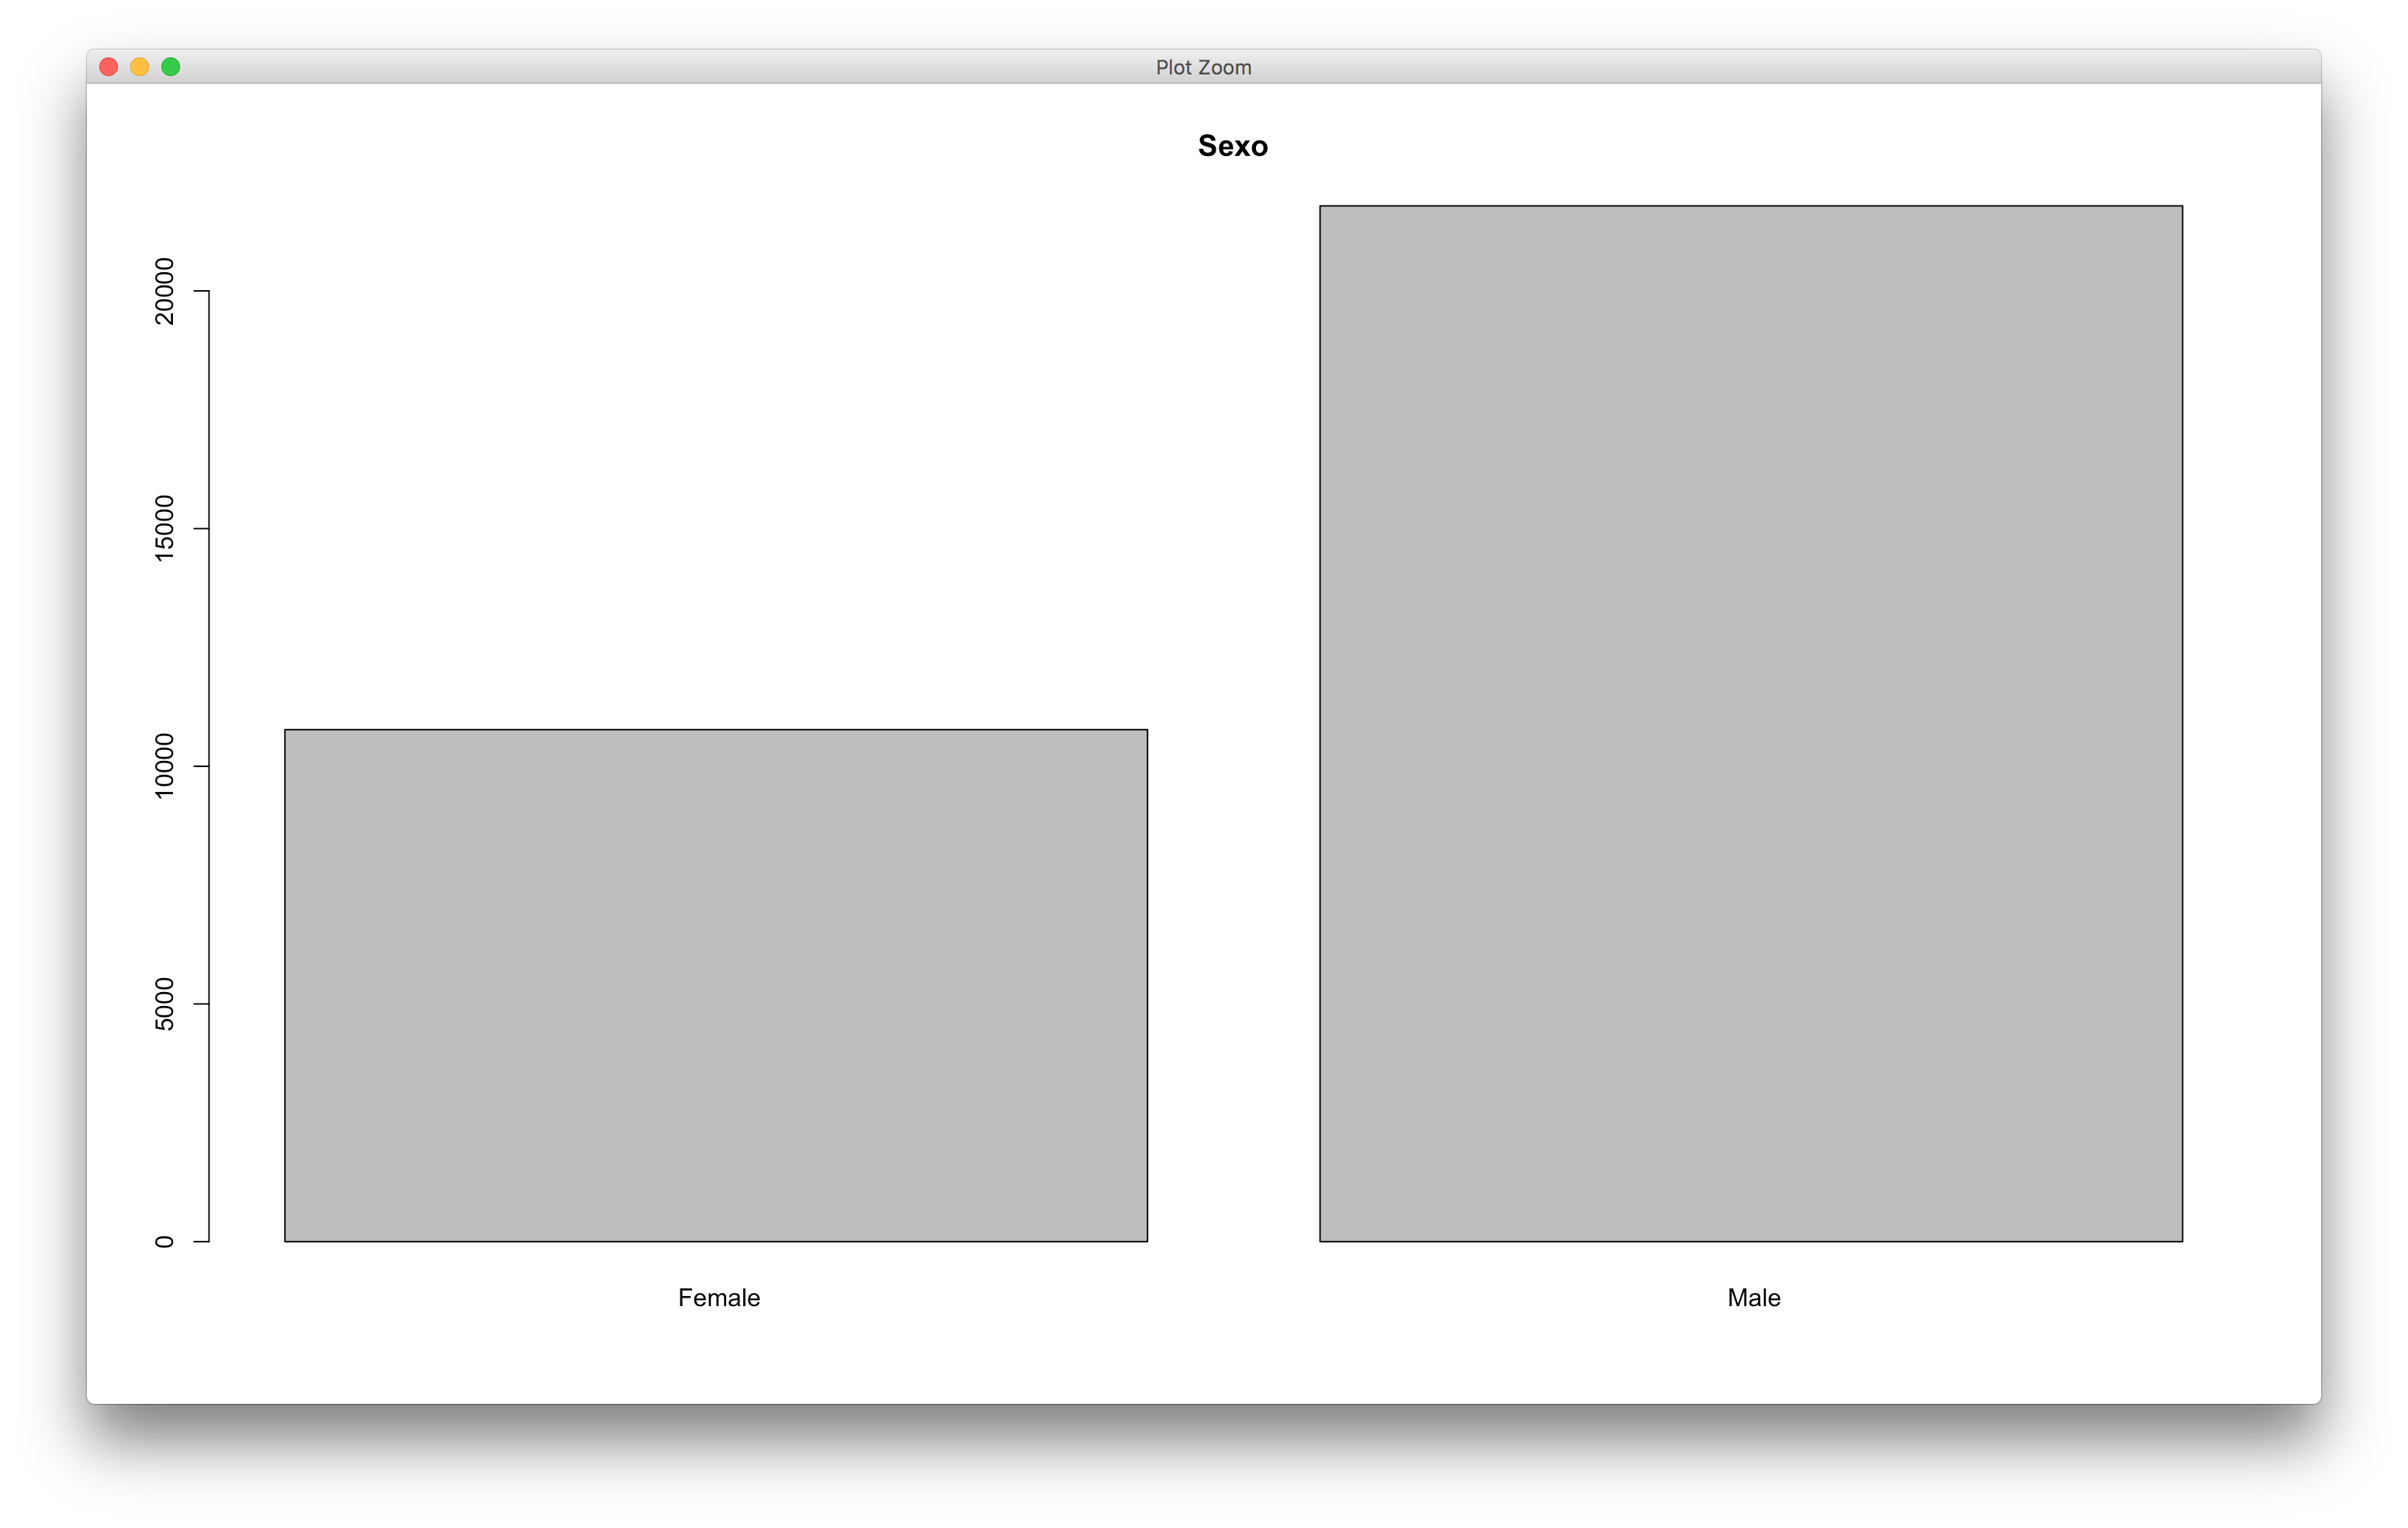
\includegraphics[scale=0.4]{graficas/sexo}}
 \end{center}
 \begin{center}
   \hbox{\hspace{-5.8em}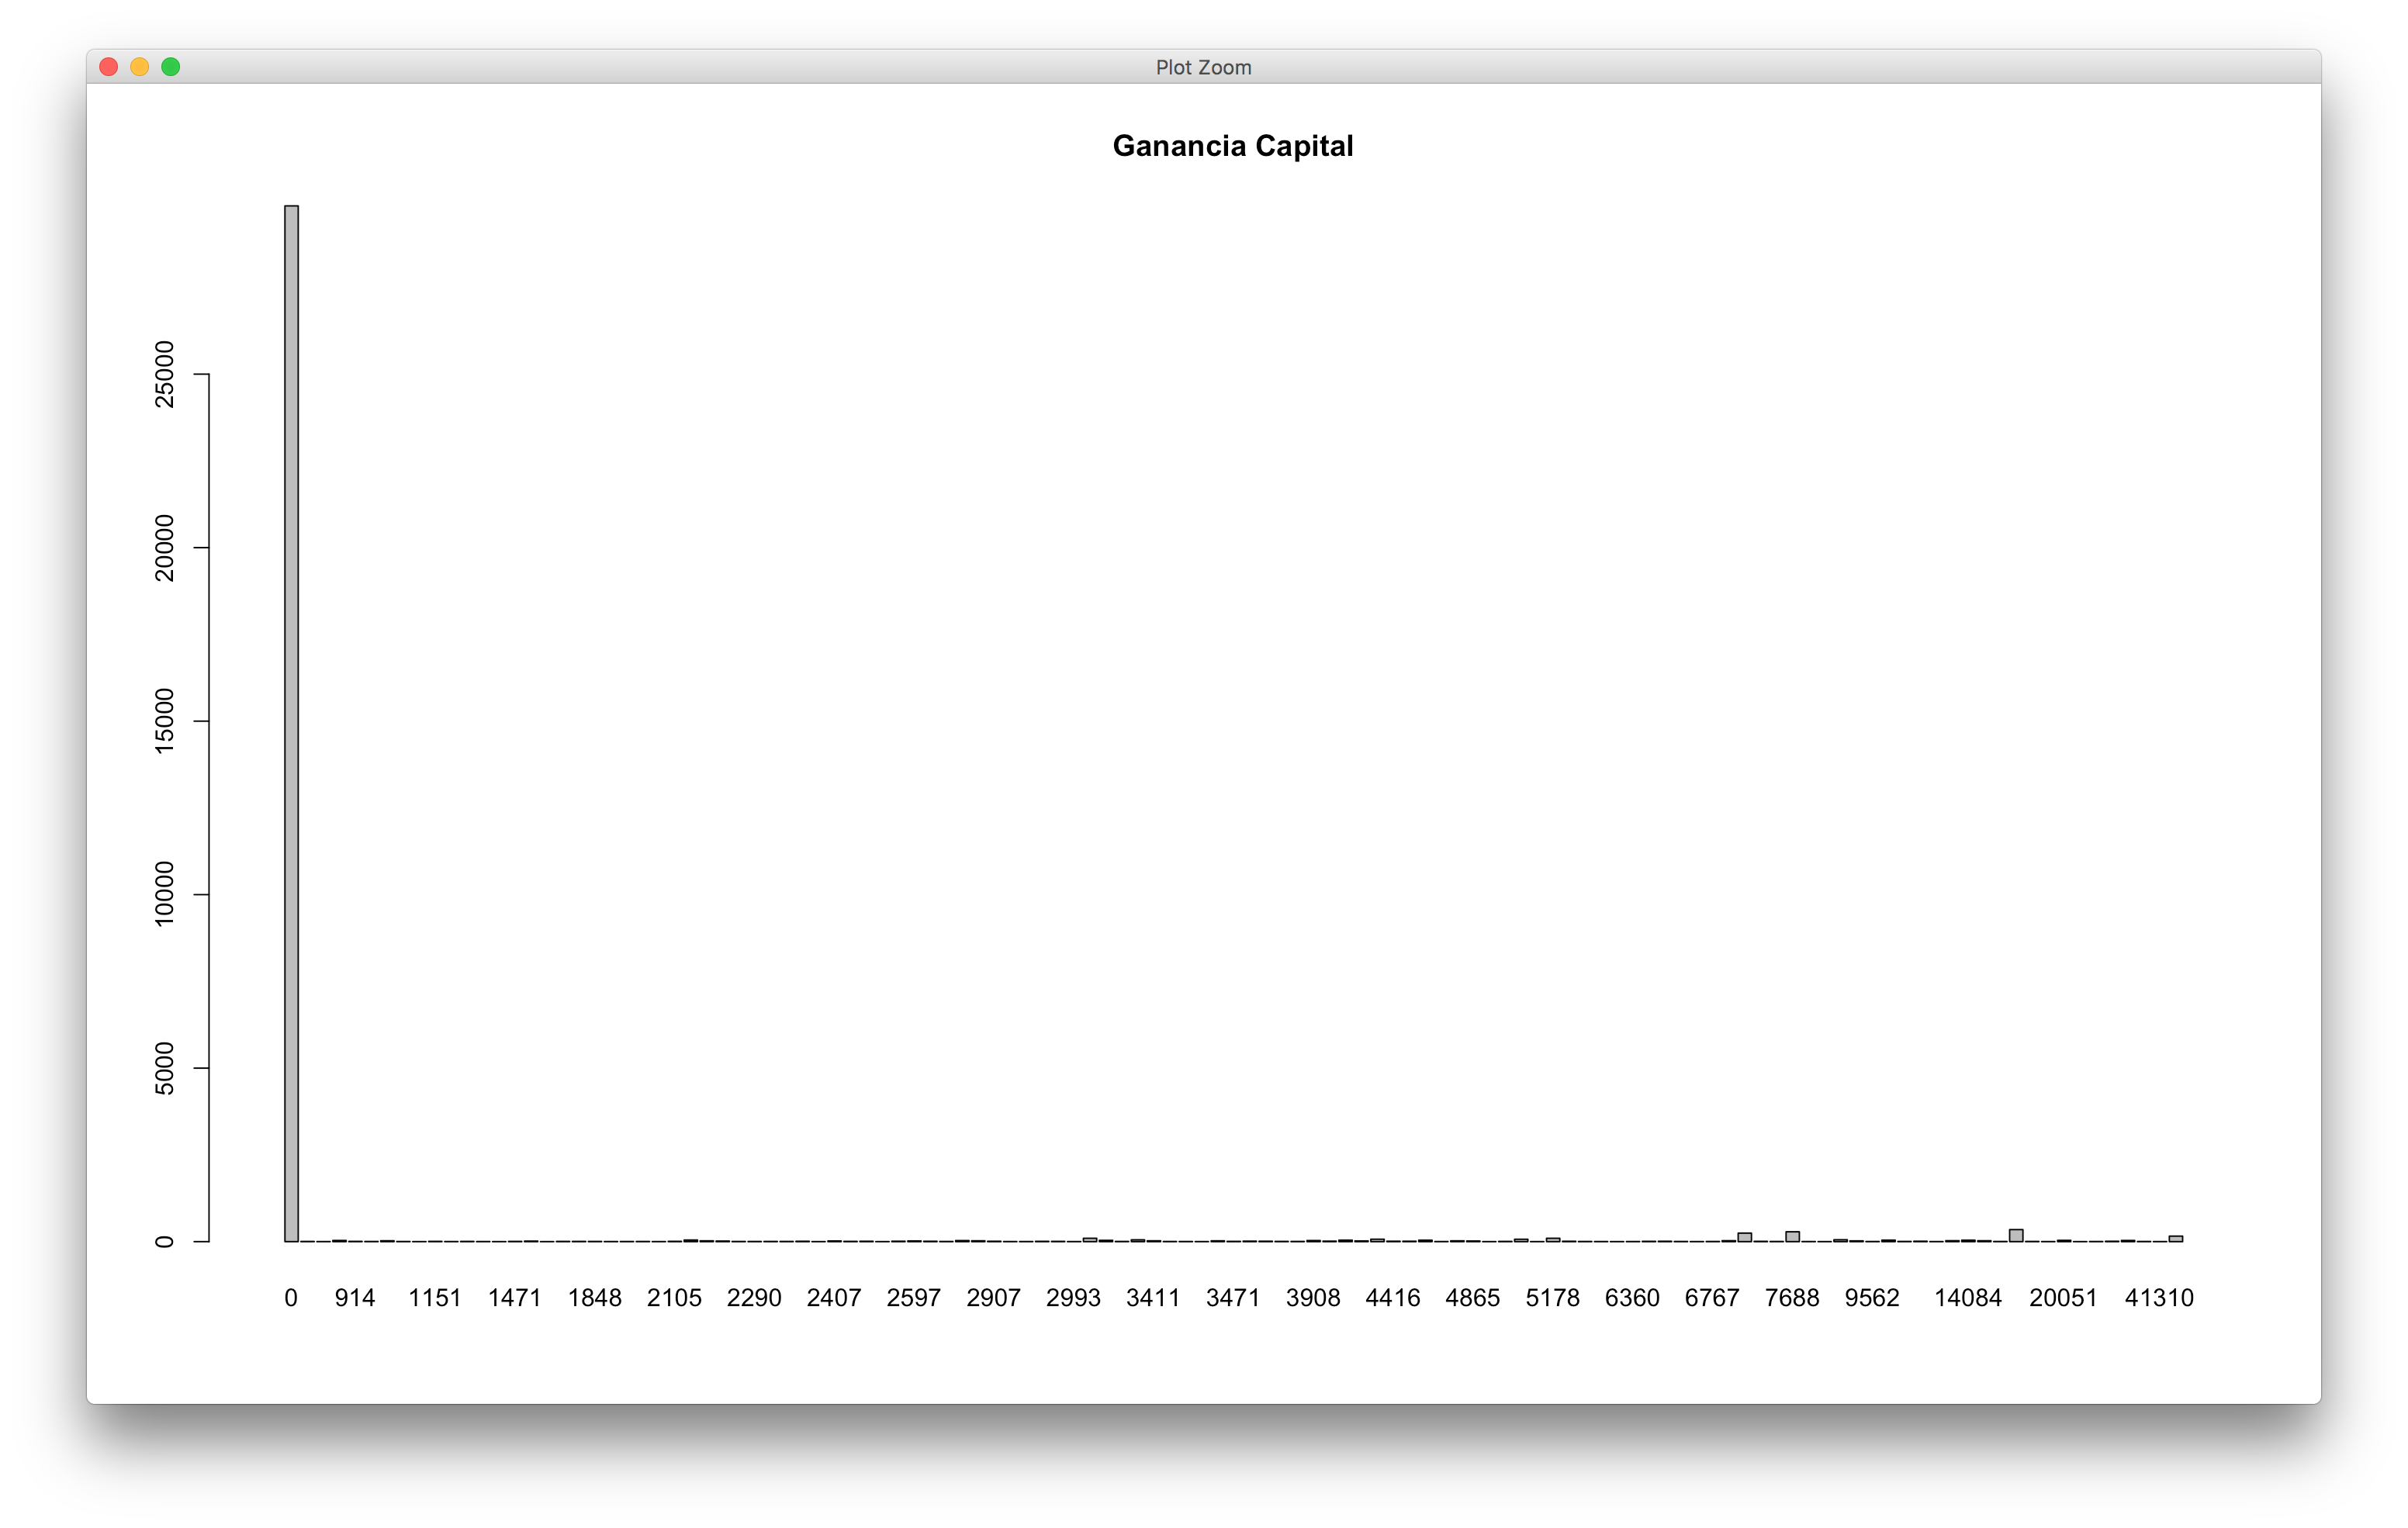
\includegraphics[scale=0.4]{graficas/gananciaCapital}}
 \end{center}
 \begin{center}
   \hbox{\hspace{-5.8em}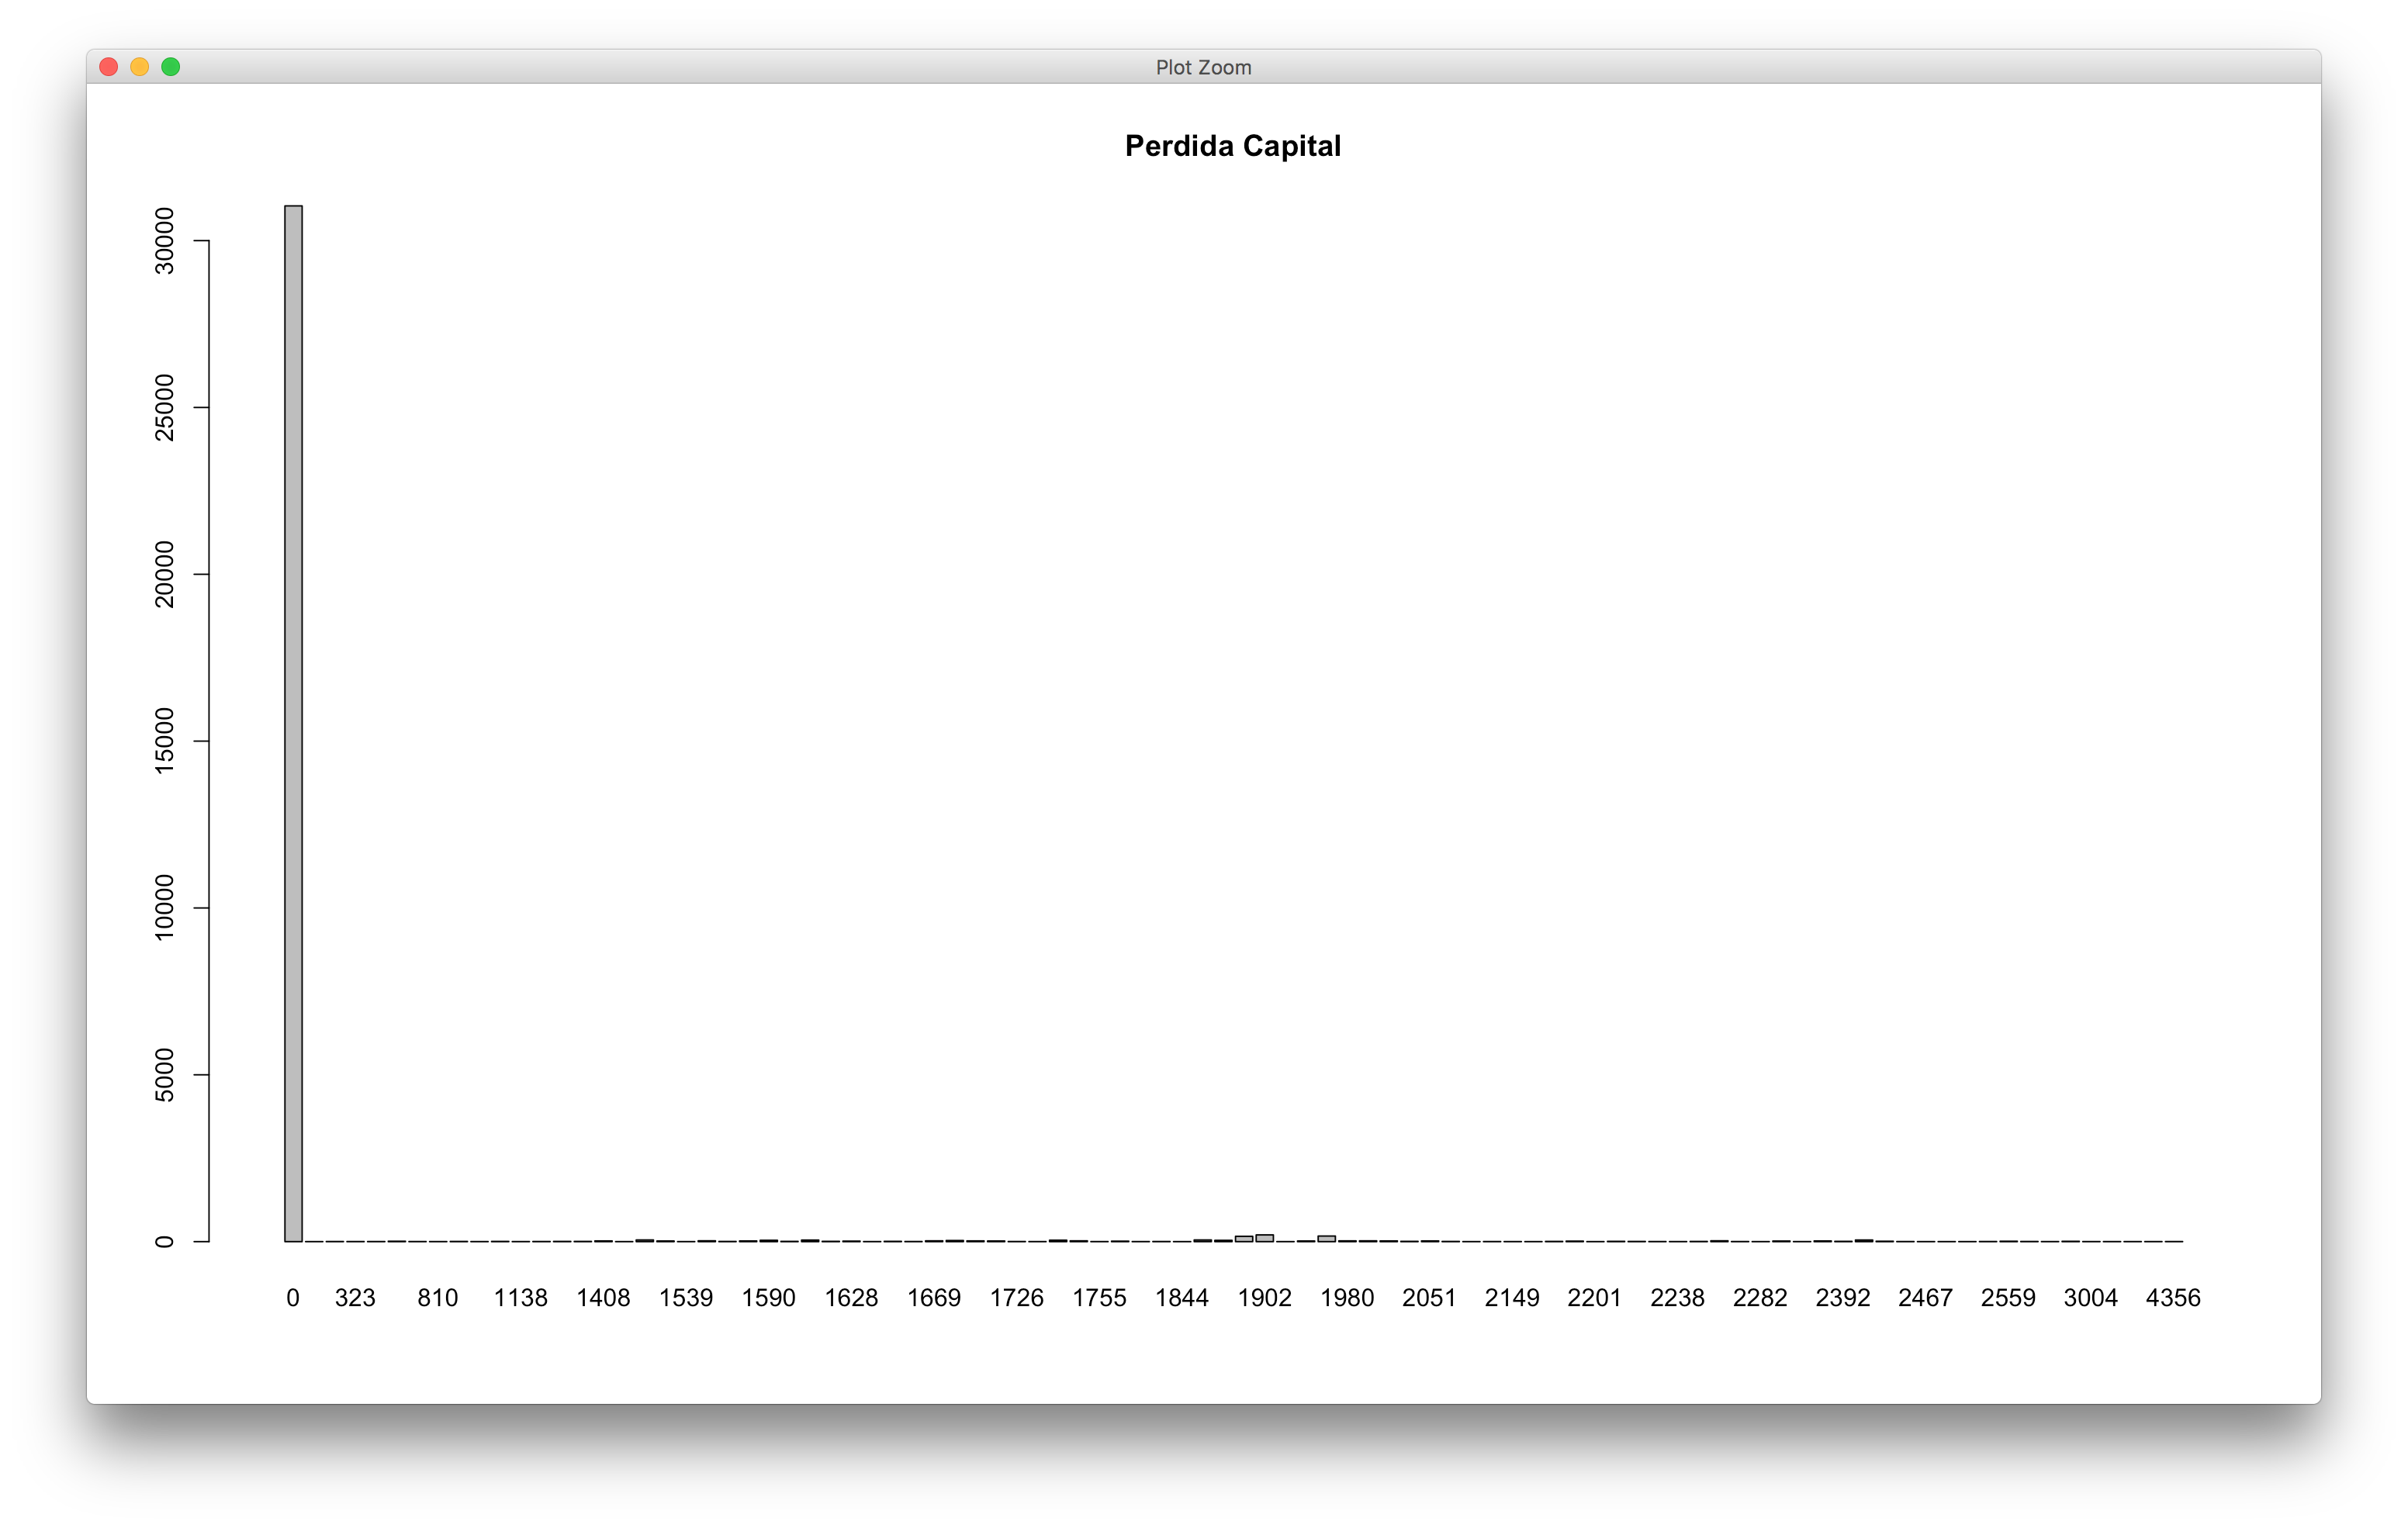
\includegraphics[scale=0.4]{graficas/perdidaCapital}}
 \end{center}
 \begin{center}
   \hbox{\hspace{-5.8em}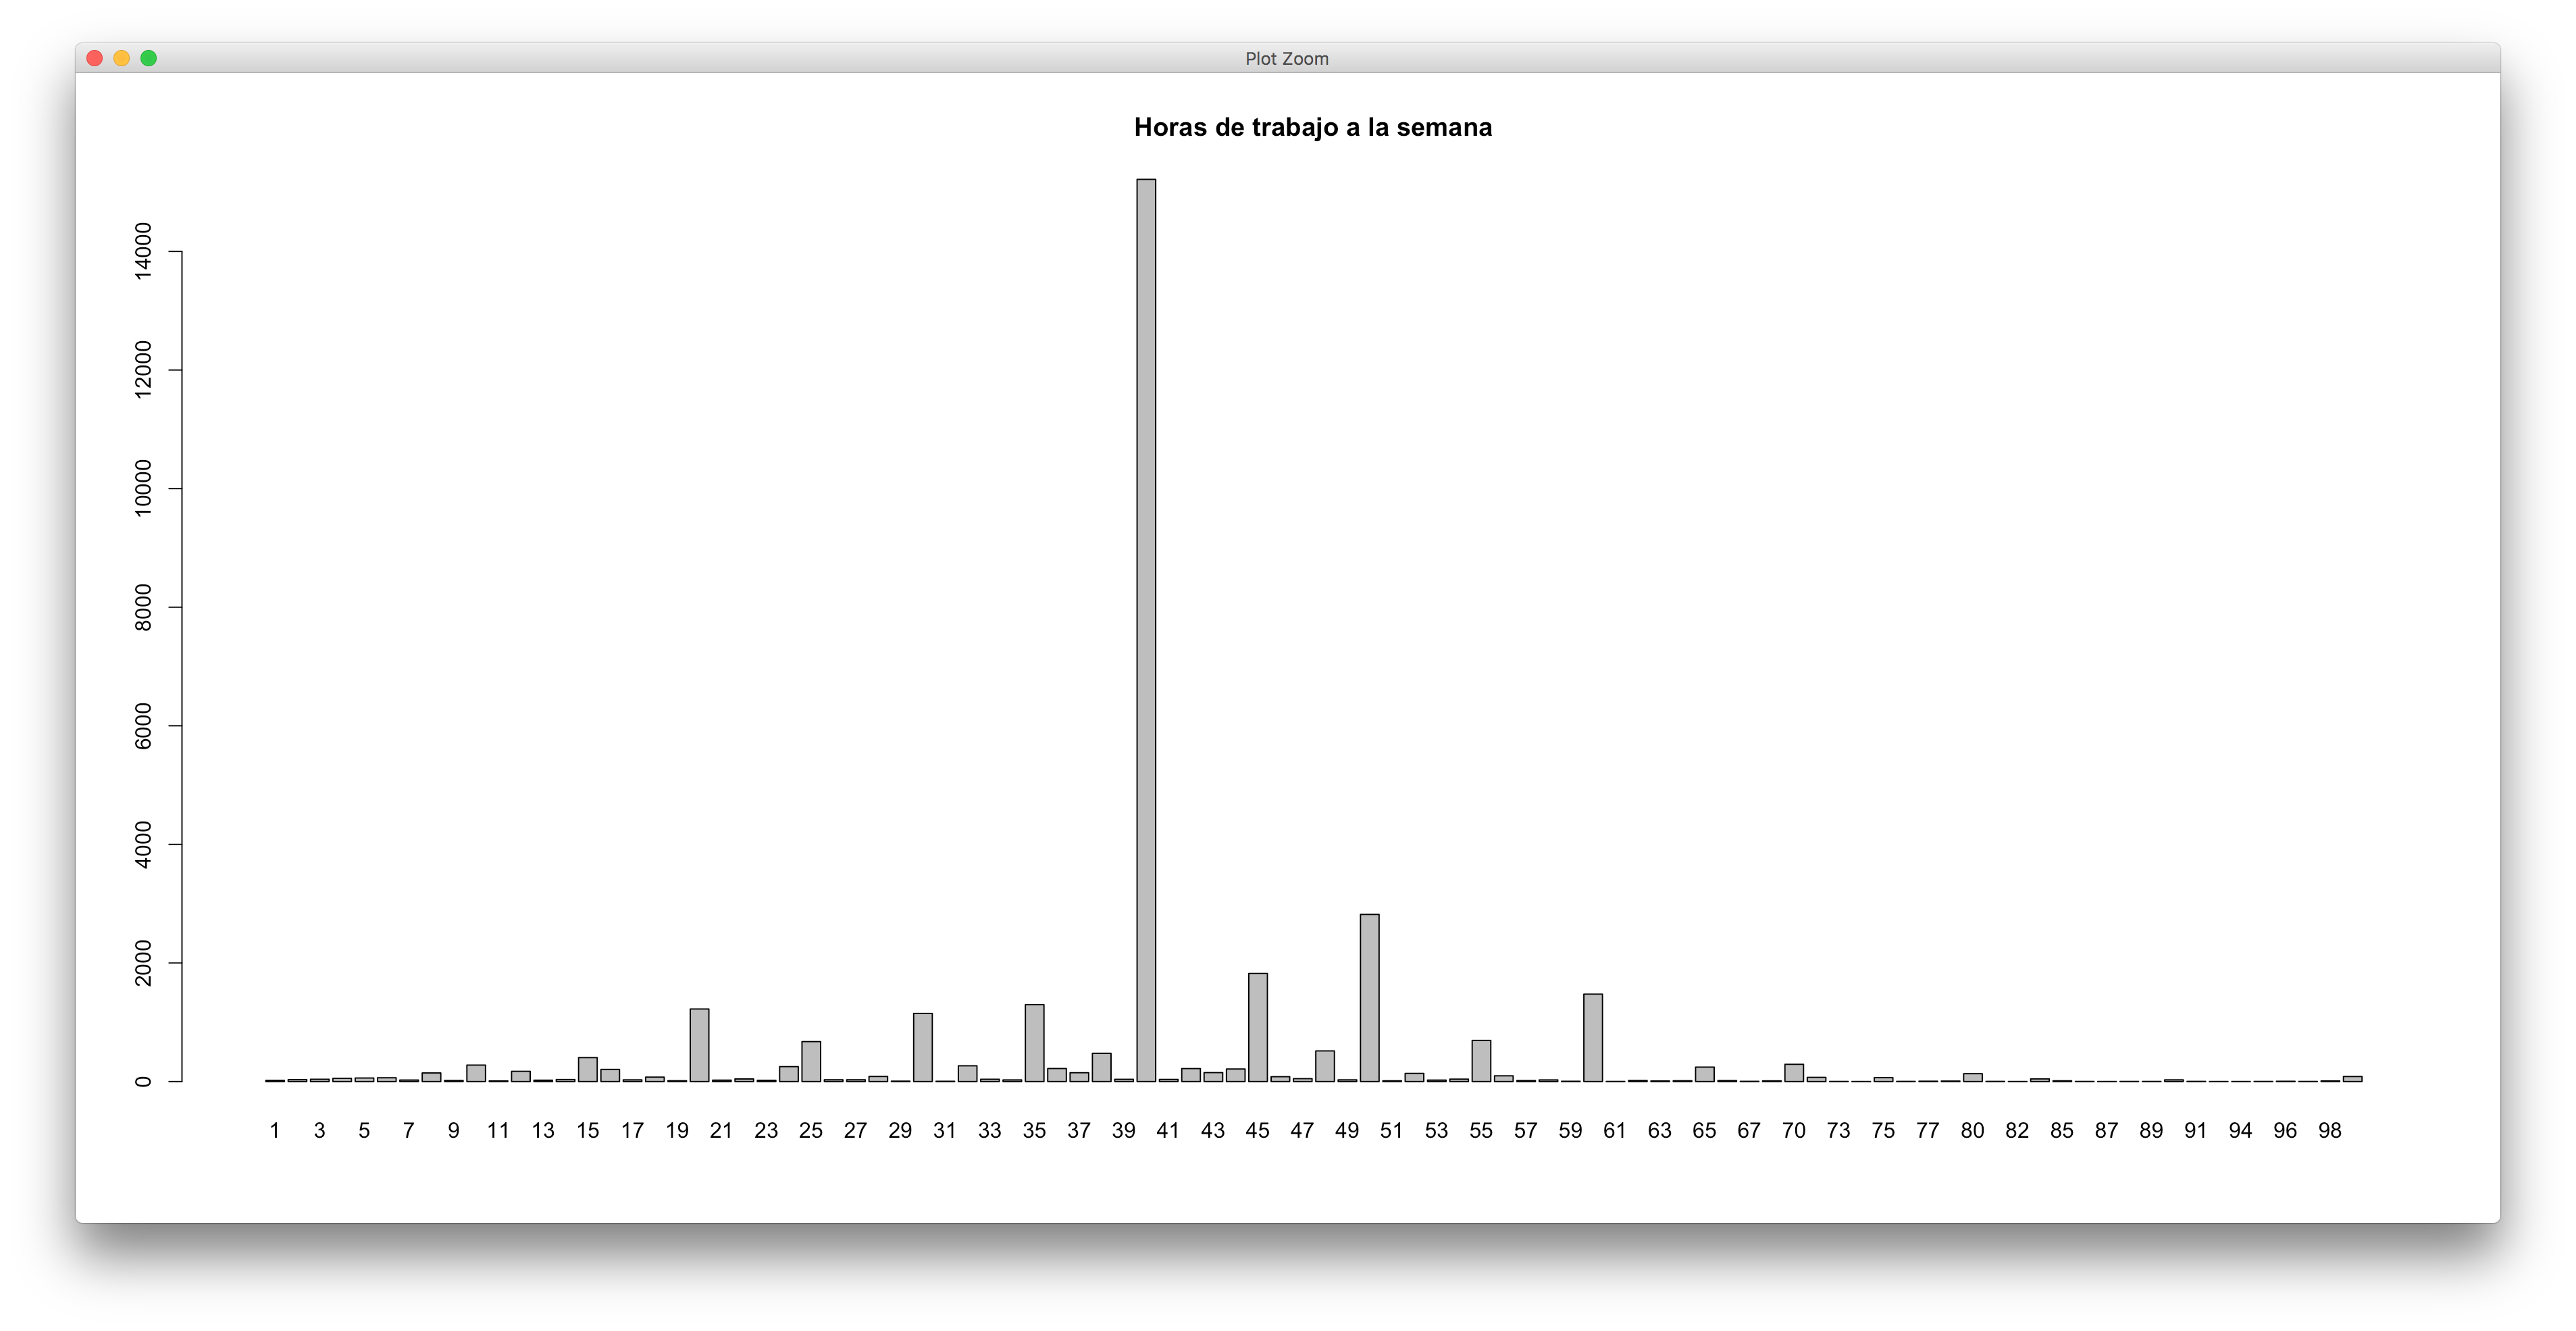
\includegraphics[scale=0.33]{graficas/horasALaSemana}}
 \end{center}
 \begin{center}
   \hbox{\hspace{-5.8em}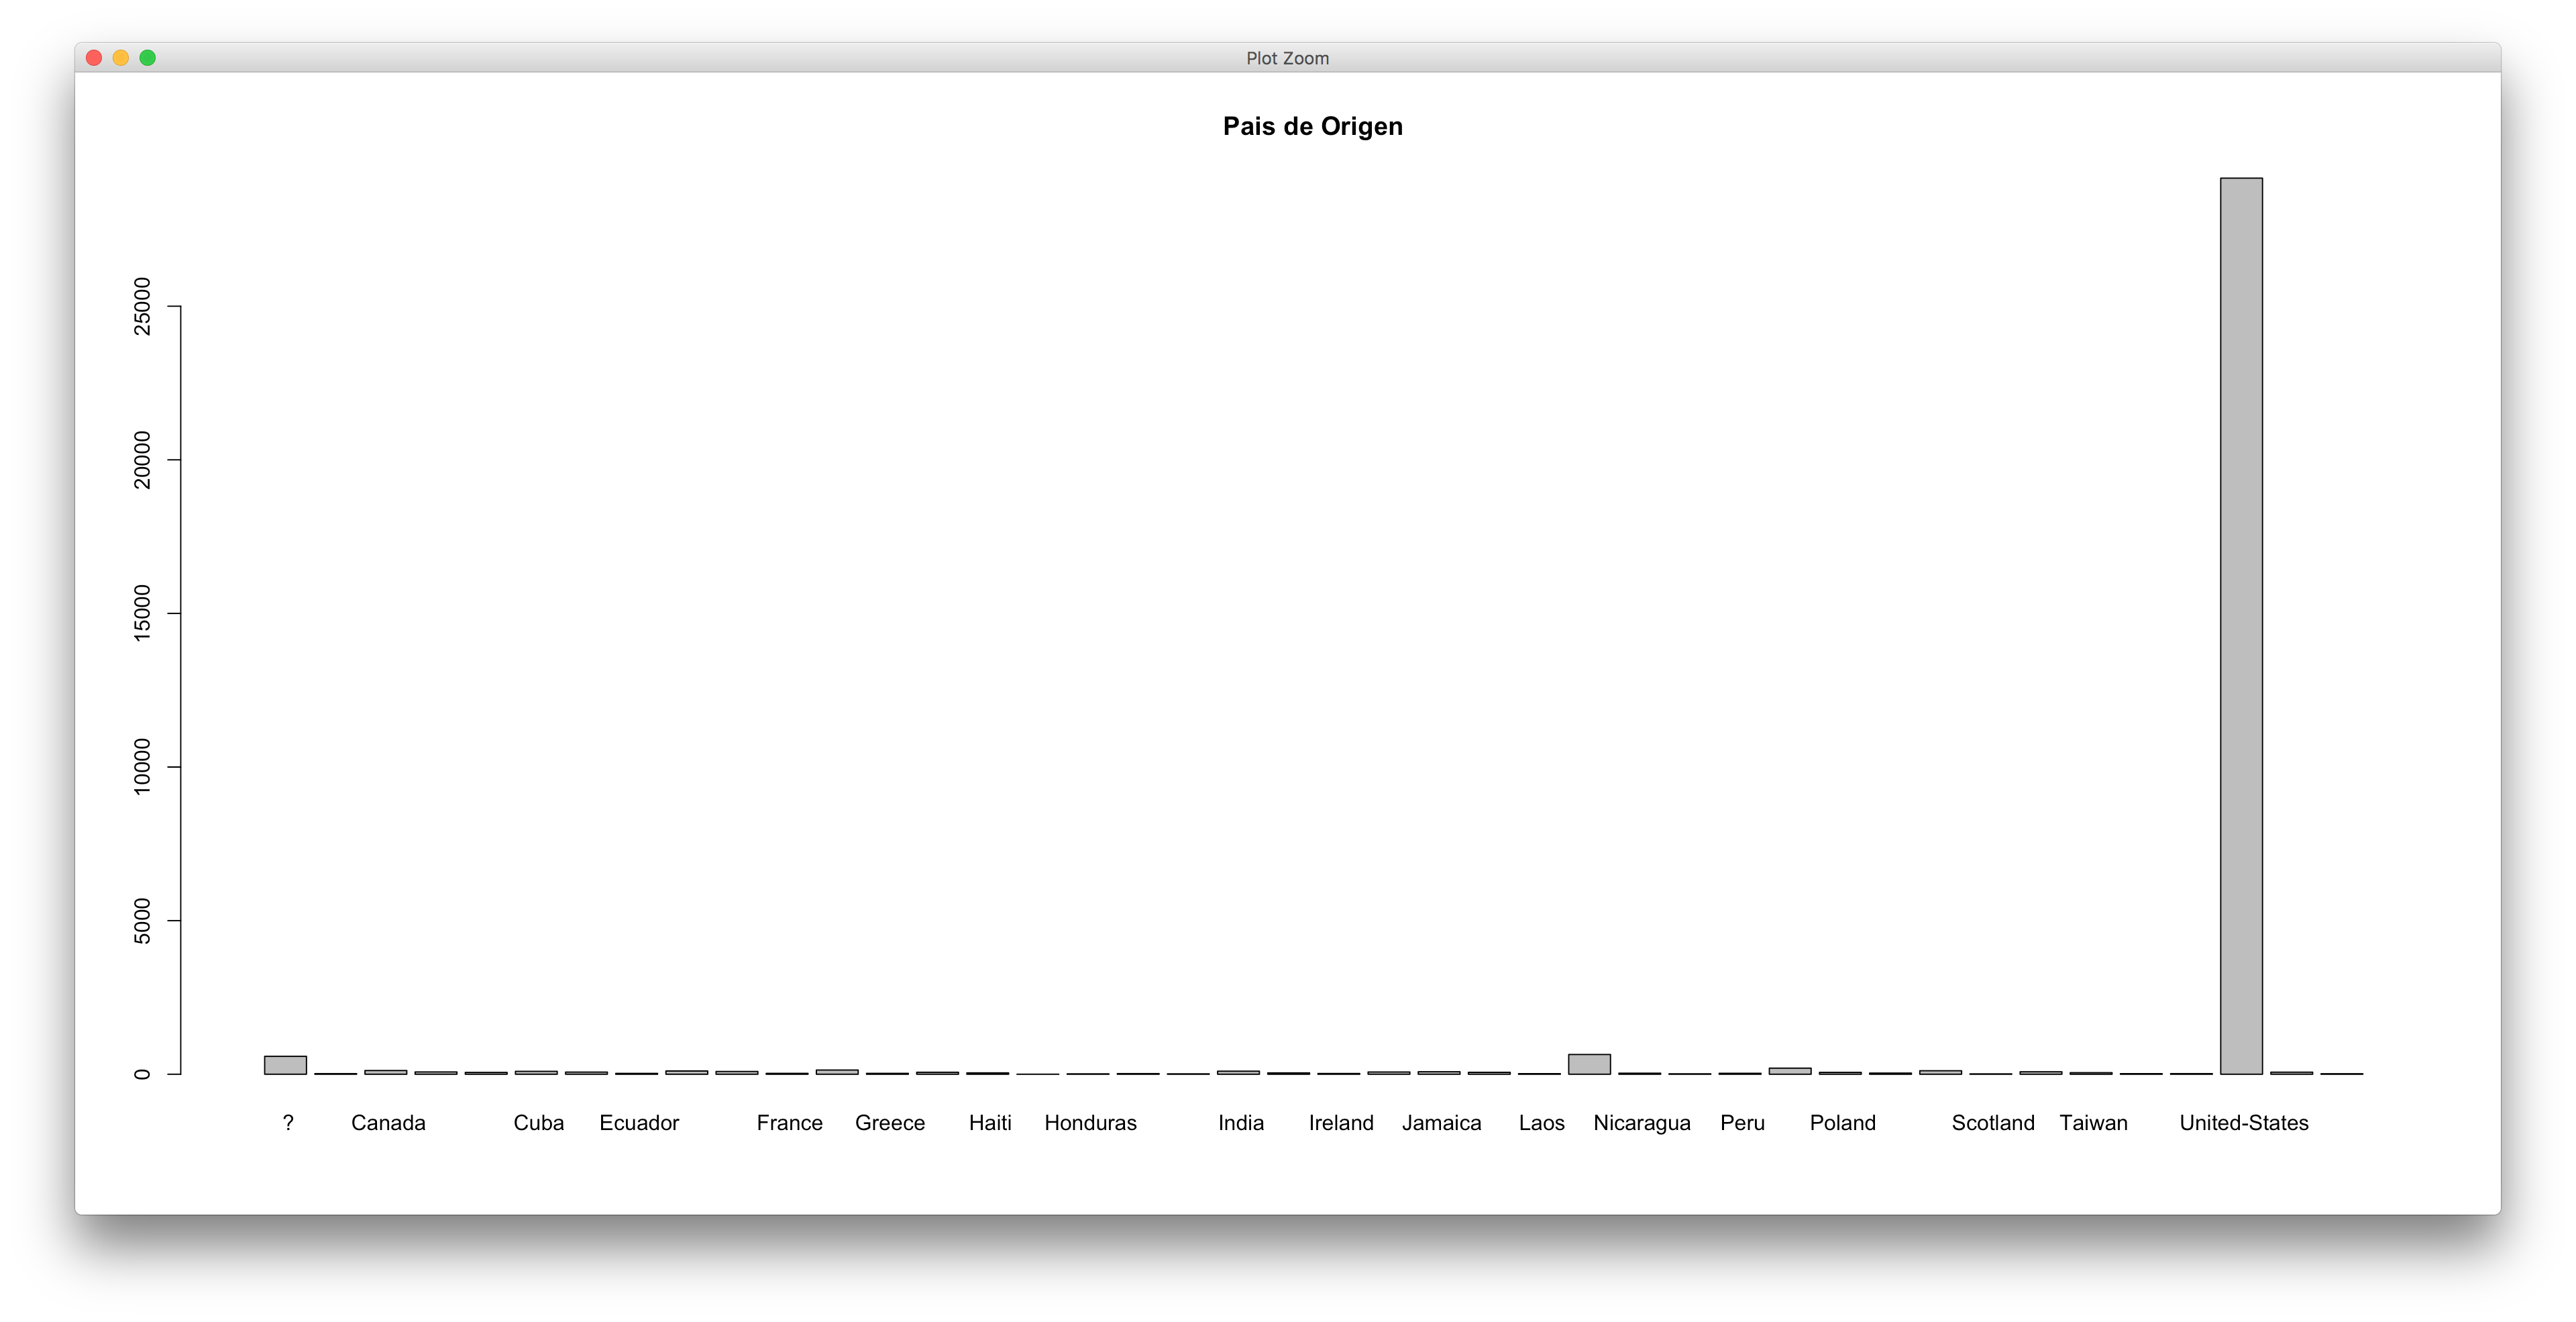
\includegraphics[scale=0.33]{graficas/paisDeOrigen}}
 \end{center}
 \begin{center}
   \hbox{\hspace{-5.8em}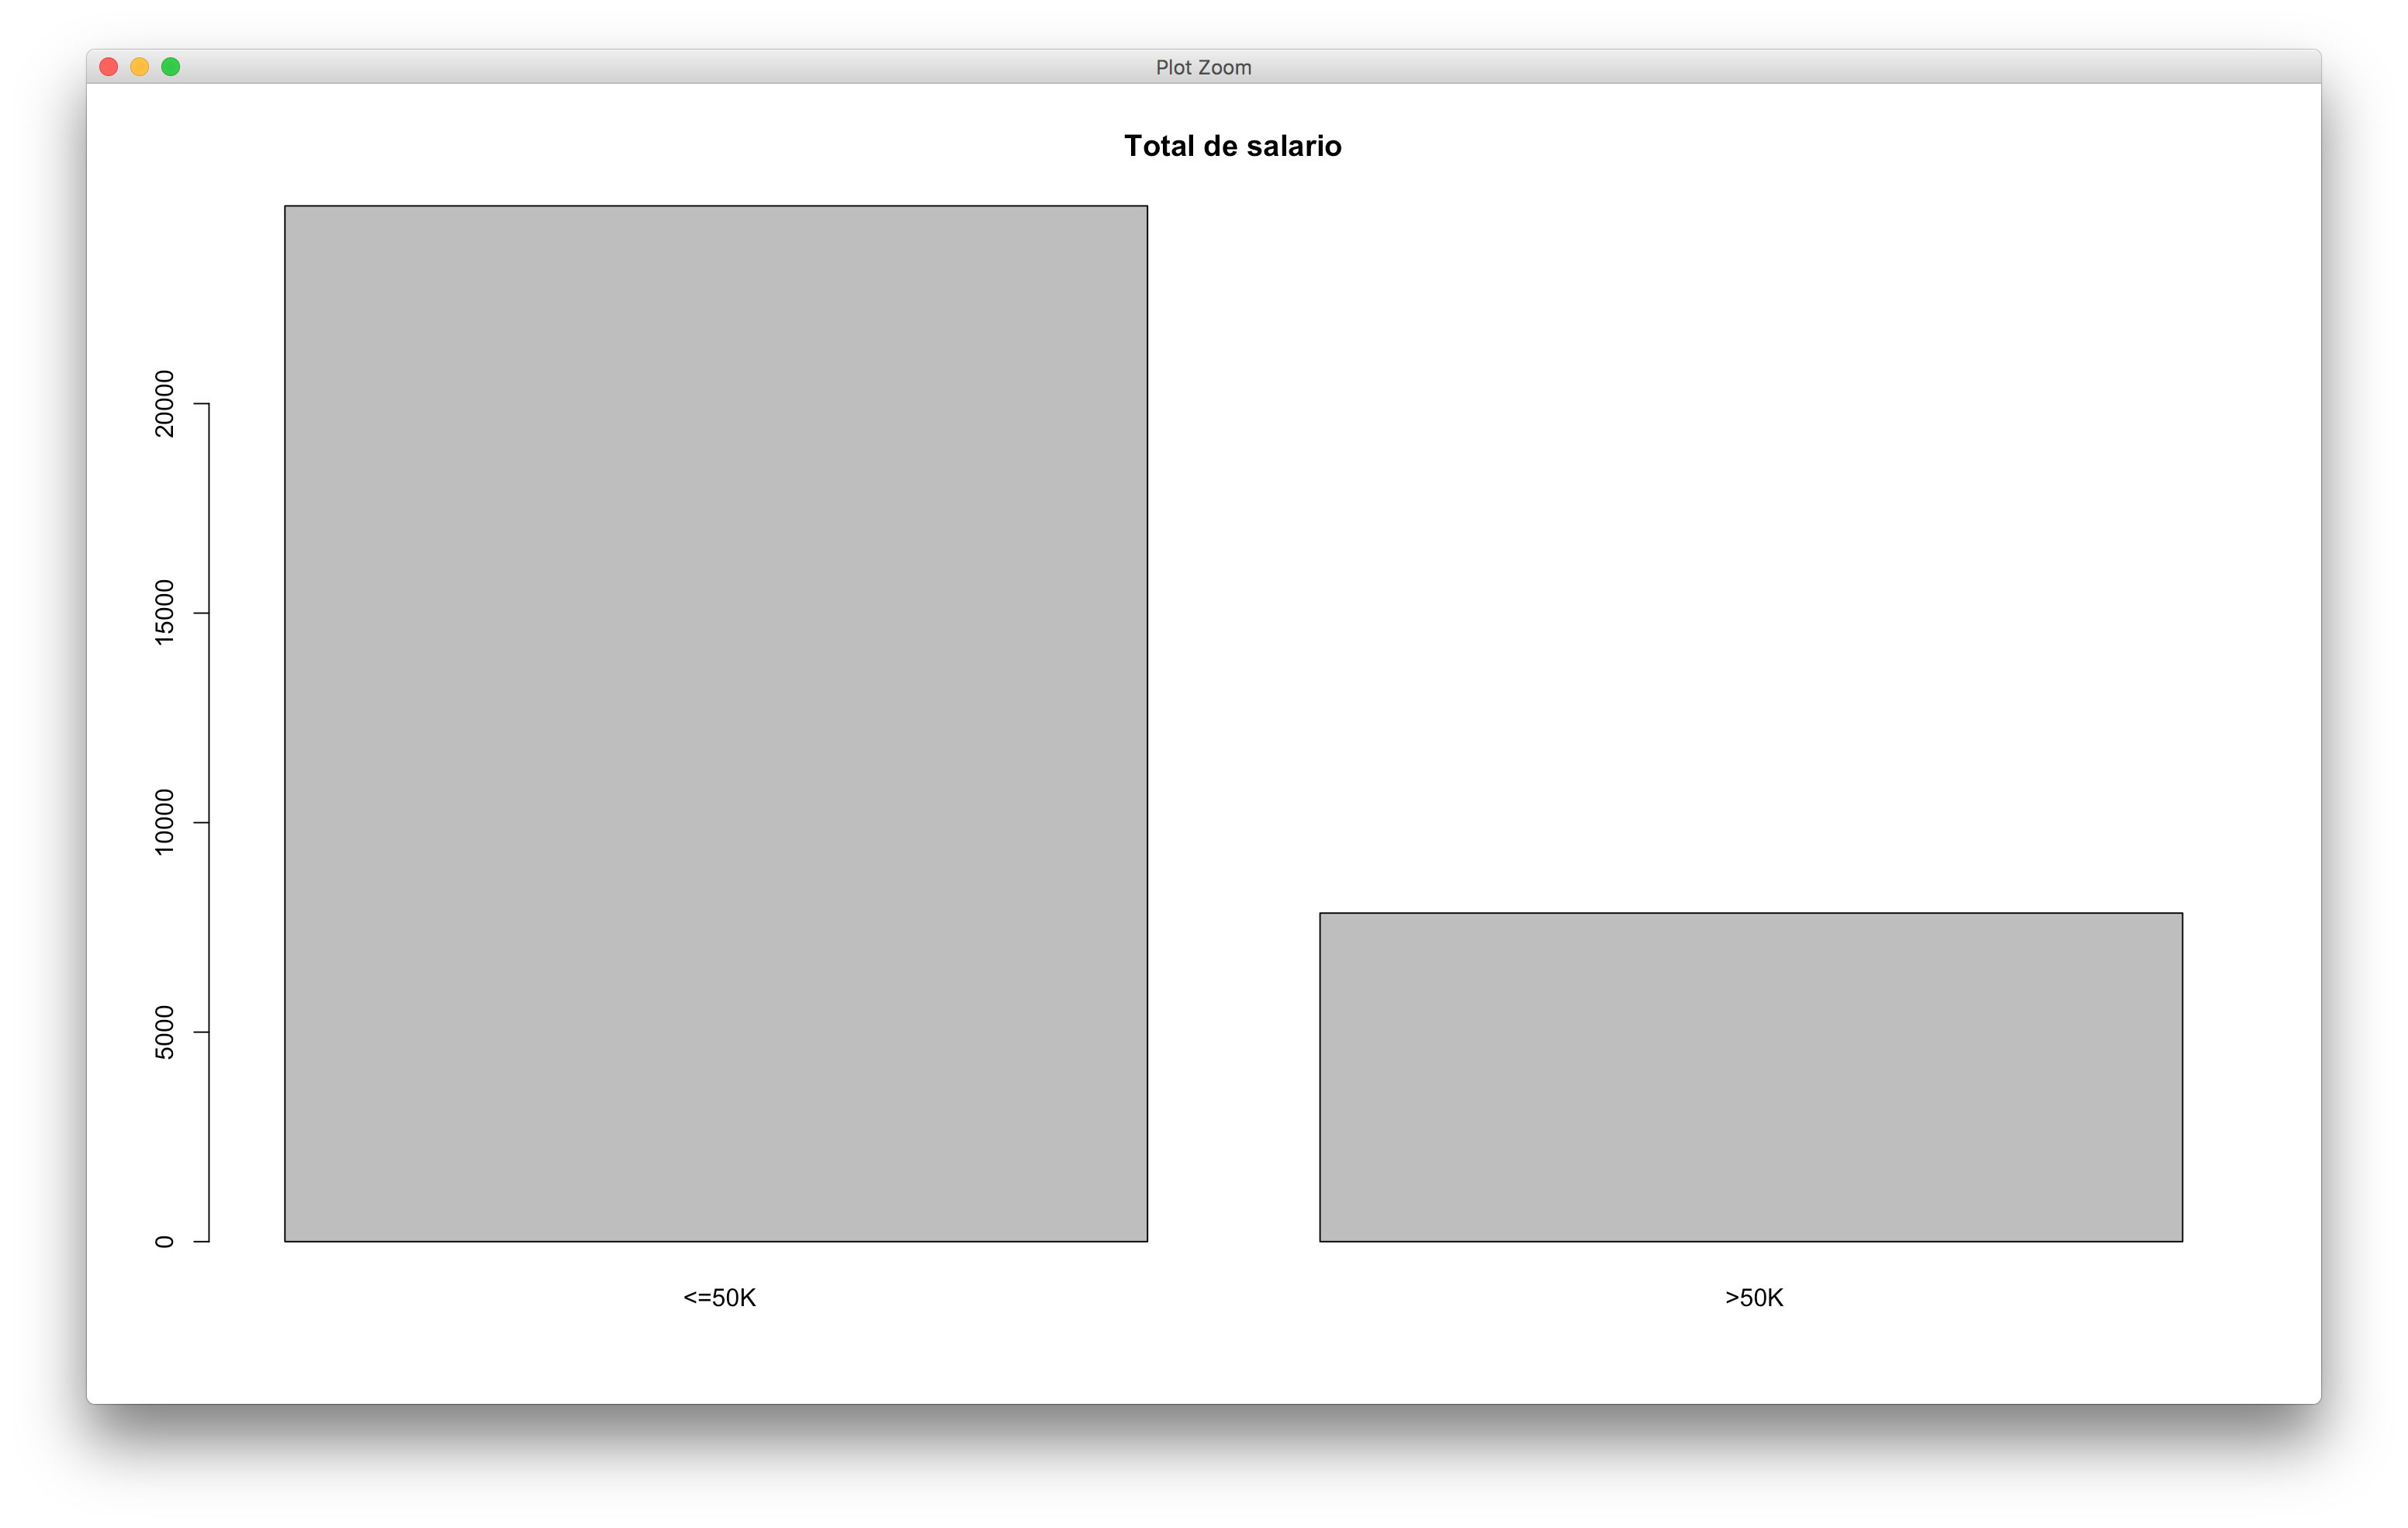
\includegraphics[scale=0.4]{graficas/totalDeSalario}}
 \end{center}

 Después de observar detalladamente estas gráficas pudimos observar que la mayoría de los individuos de este conjunto de datos tienen las siguiente características: son hombres con edad de 23 a 40 años, los cuales trabajan en el sector privado, con un grado de educación de preparatoria, están casados, son de raza blanca, trabajan 40 horas a la semana y su país de origen es Estados Unidos.

Podemos observar que {\it education} es lo mismo que {\it education\_num}, es decir, si el grado en {\it education} es 'Doctorate' entonces {\it education\_num} será 16, si es 'Masters' será 14, y asi sucesivamente. Por lo que nos podremos deshacer de uno de los dos.

\subsection{Por Parejas}
  \begin{center}
    \hbox{\hspace{-5.5em}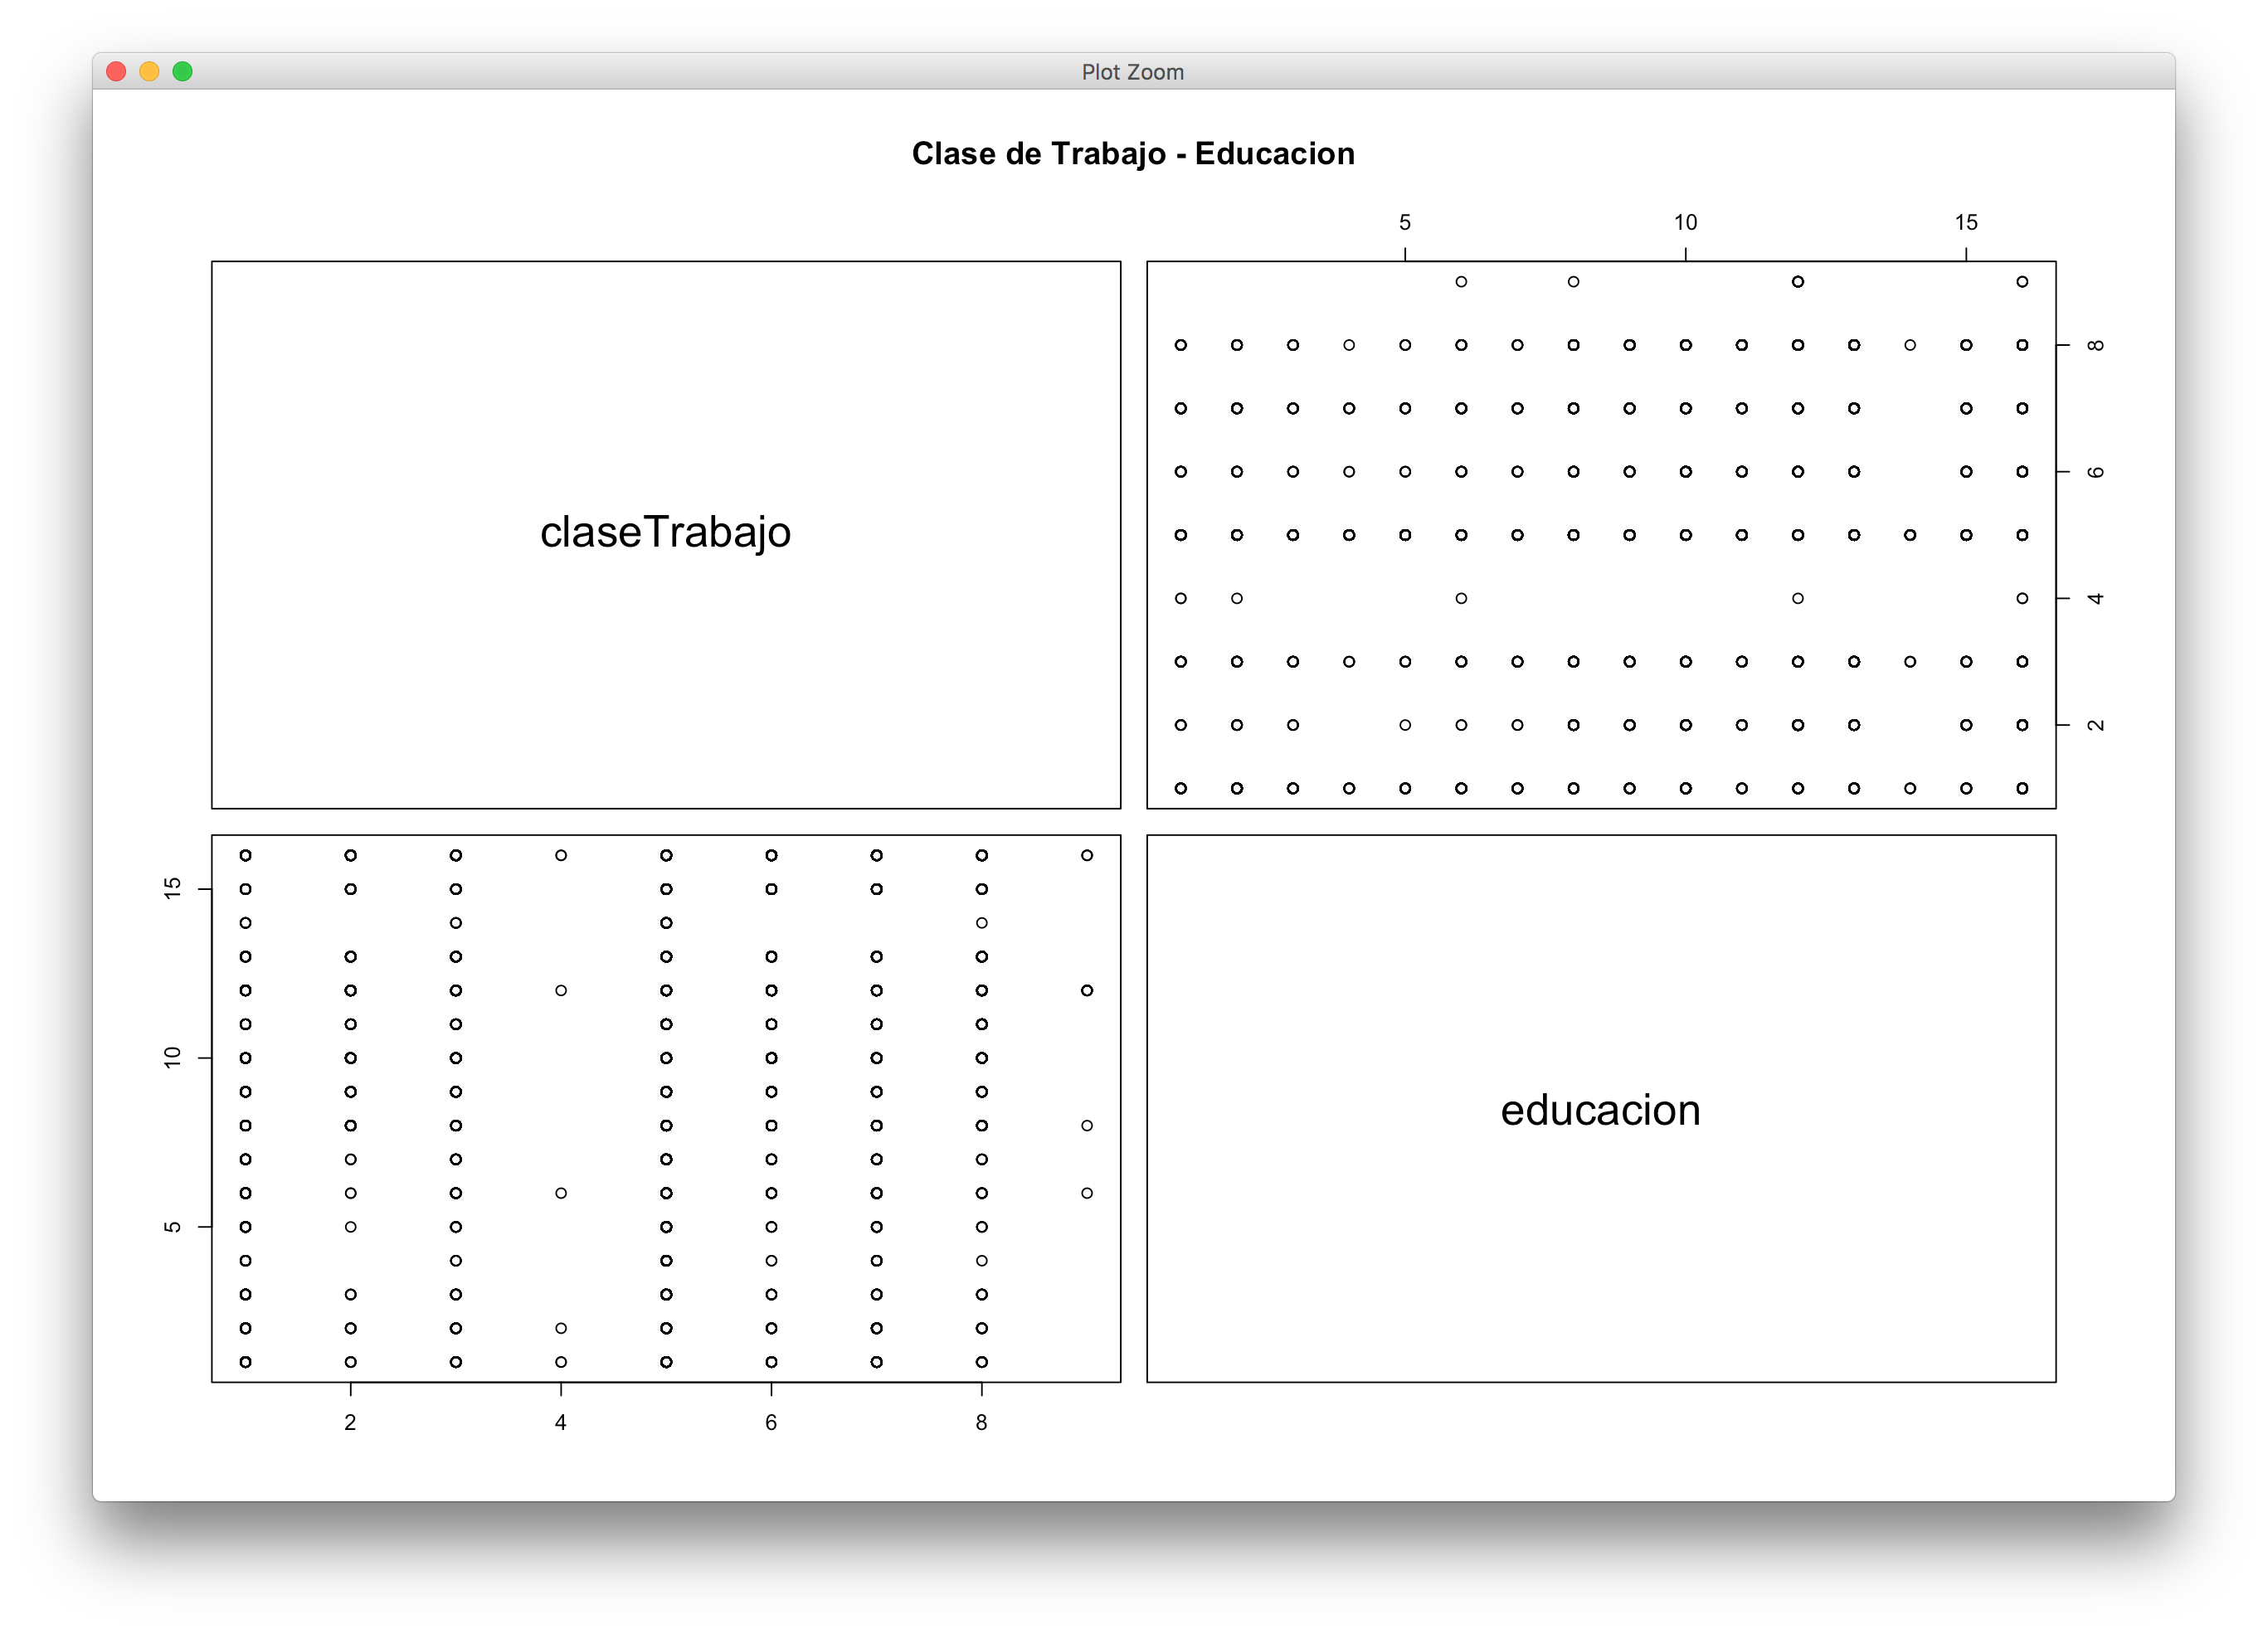
\includegraphics[scale=0.45]{graficas/ClaseTrabEdu}}
  \end{center}
  \begin{center}
    \hbox{\hspace{-5.5em}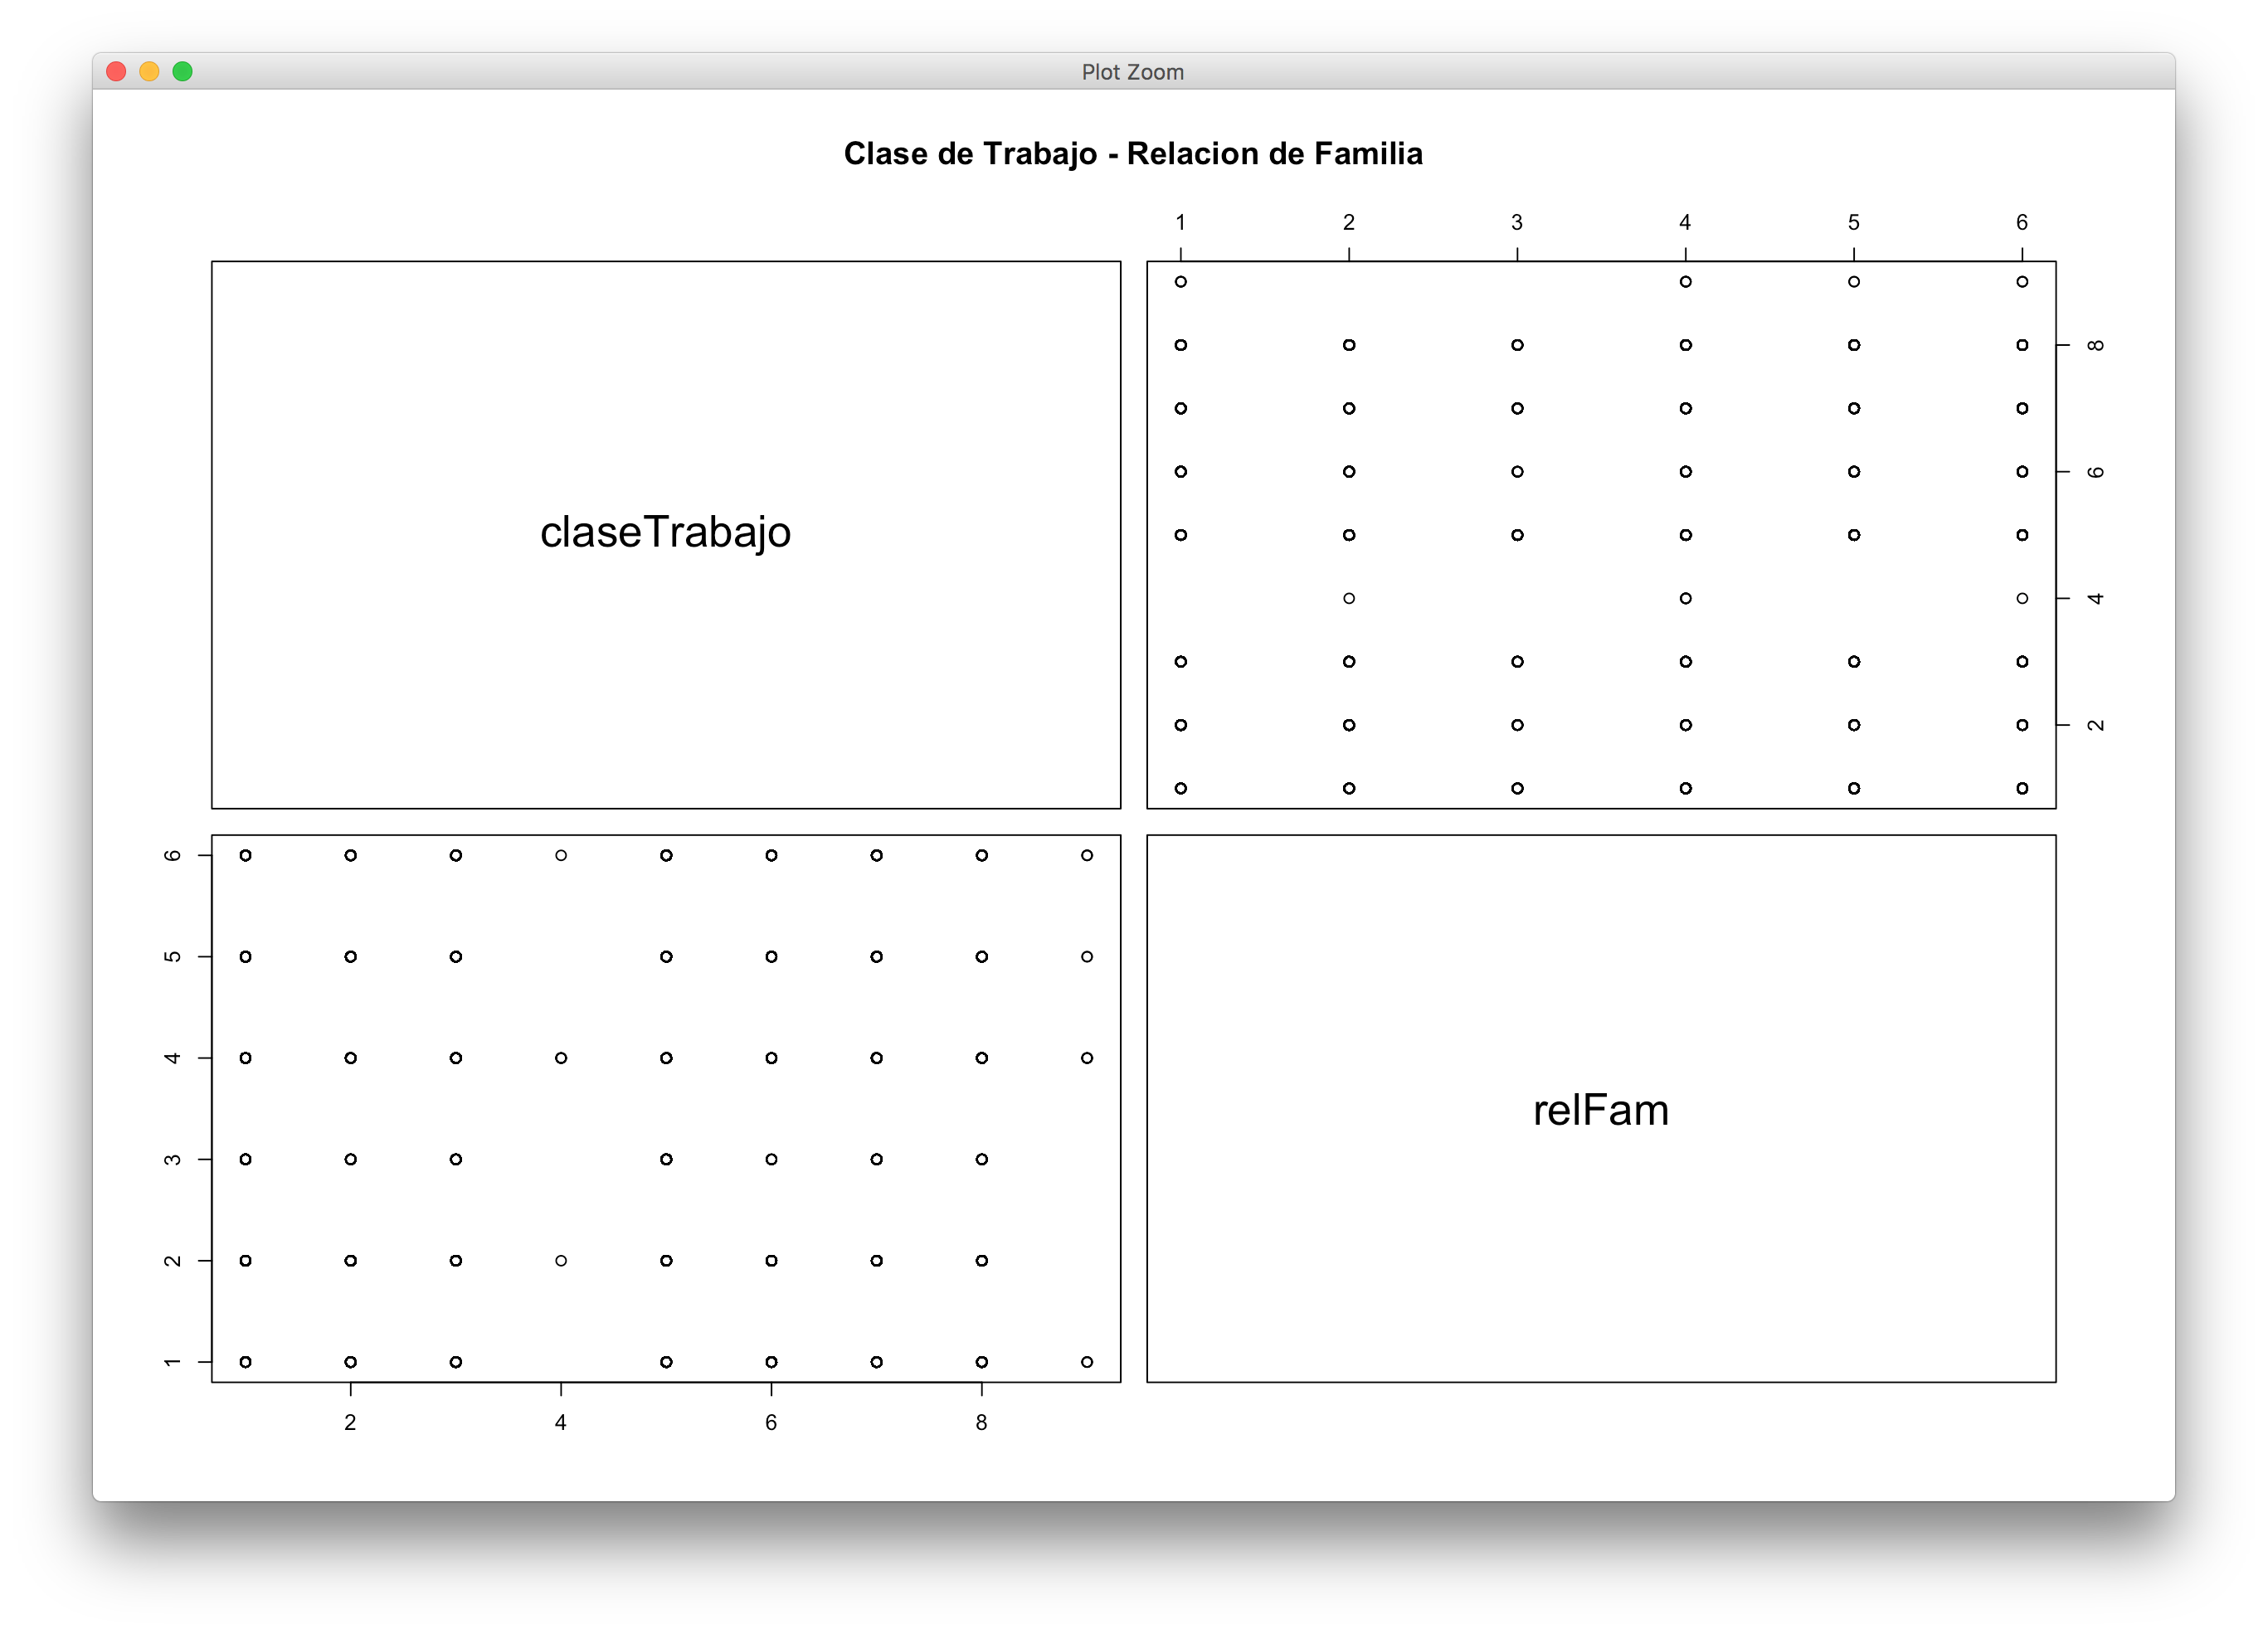
\includegraphics[scale=0.45]{graficas/claseTrabjRelSem}}
  \end{center}
  \begin{center}
    \hbox{\hspace{-5.5em}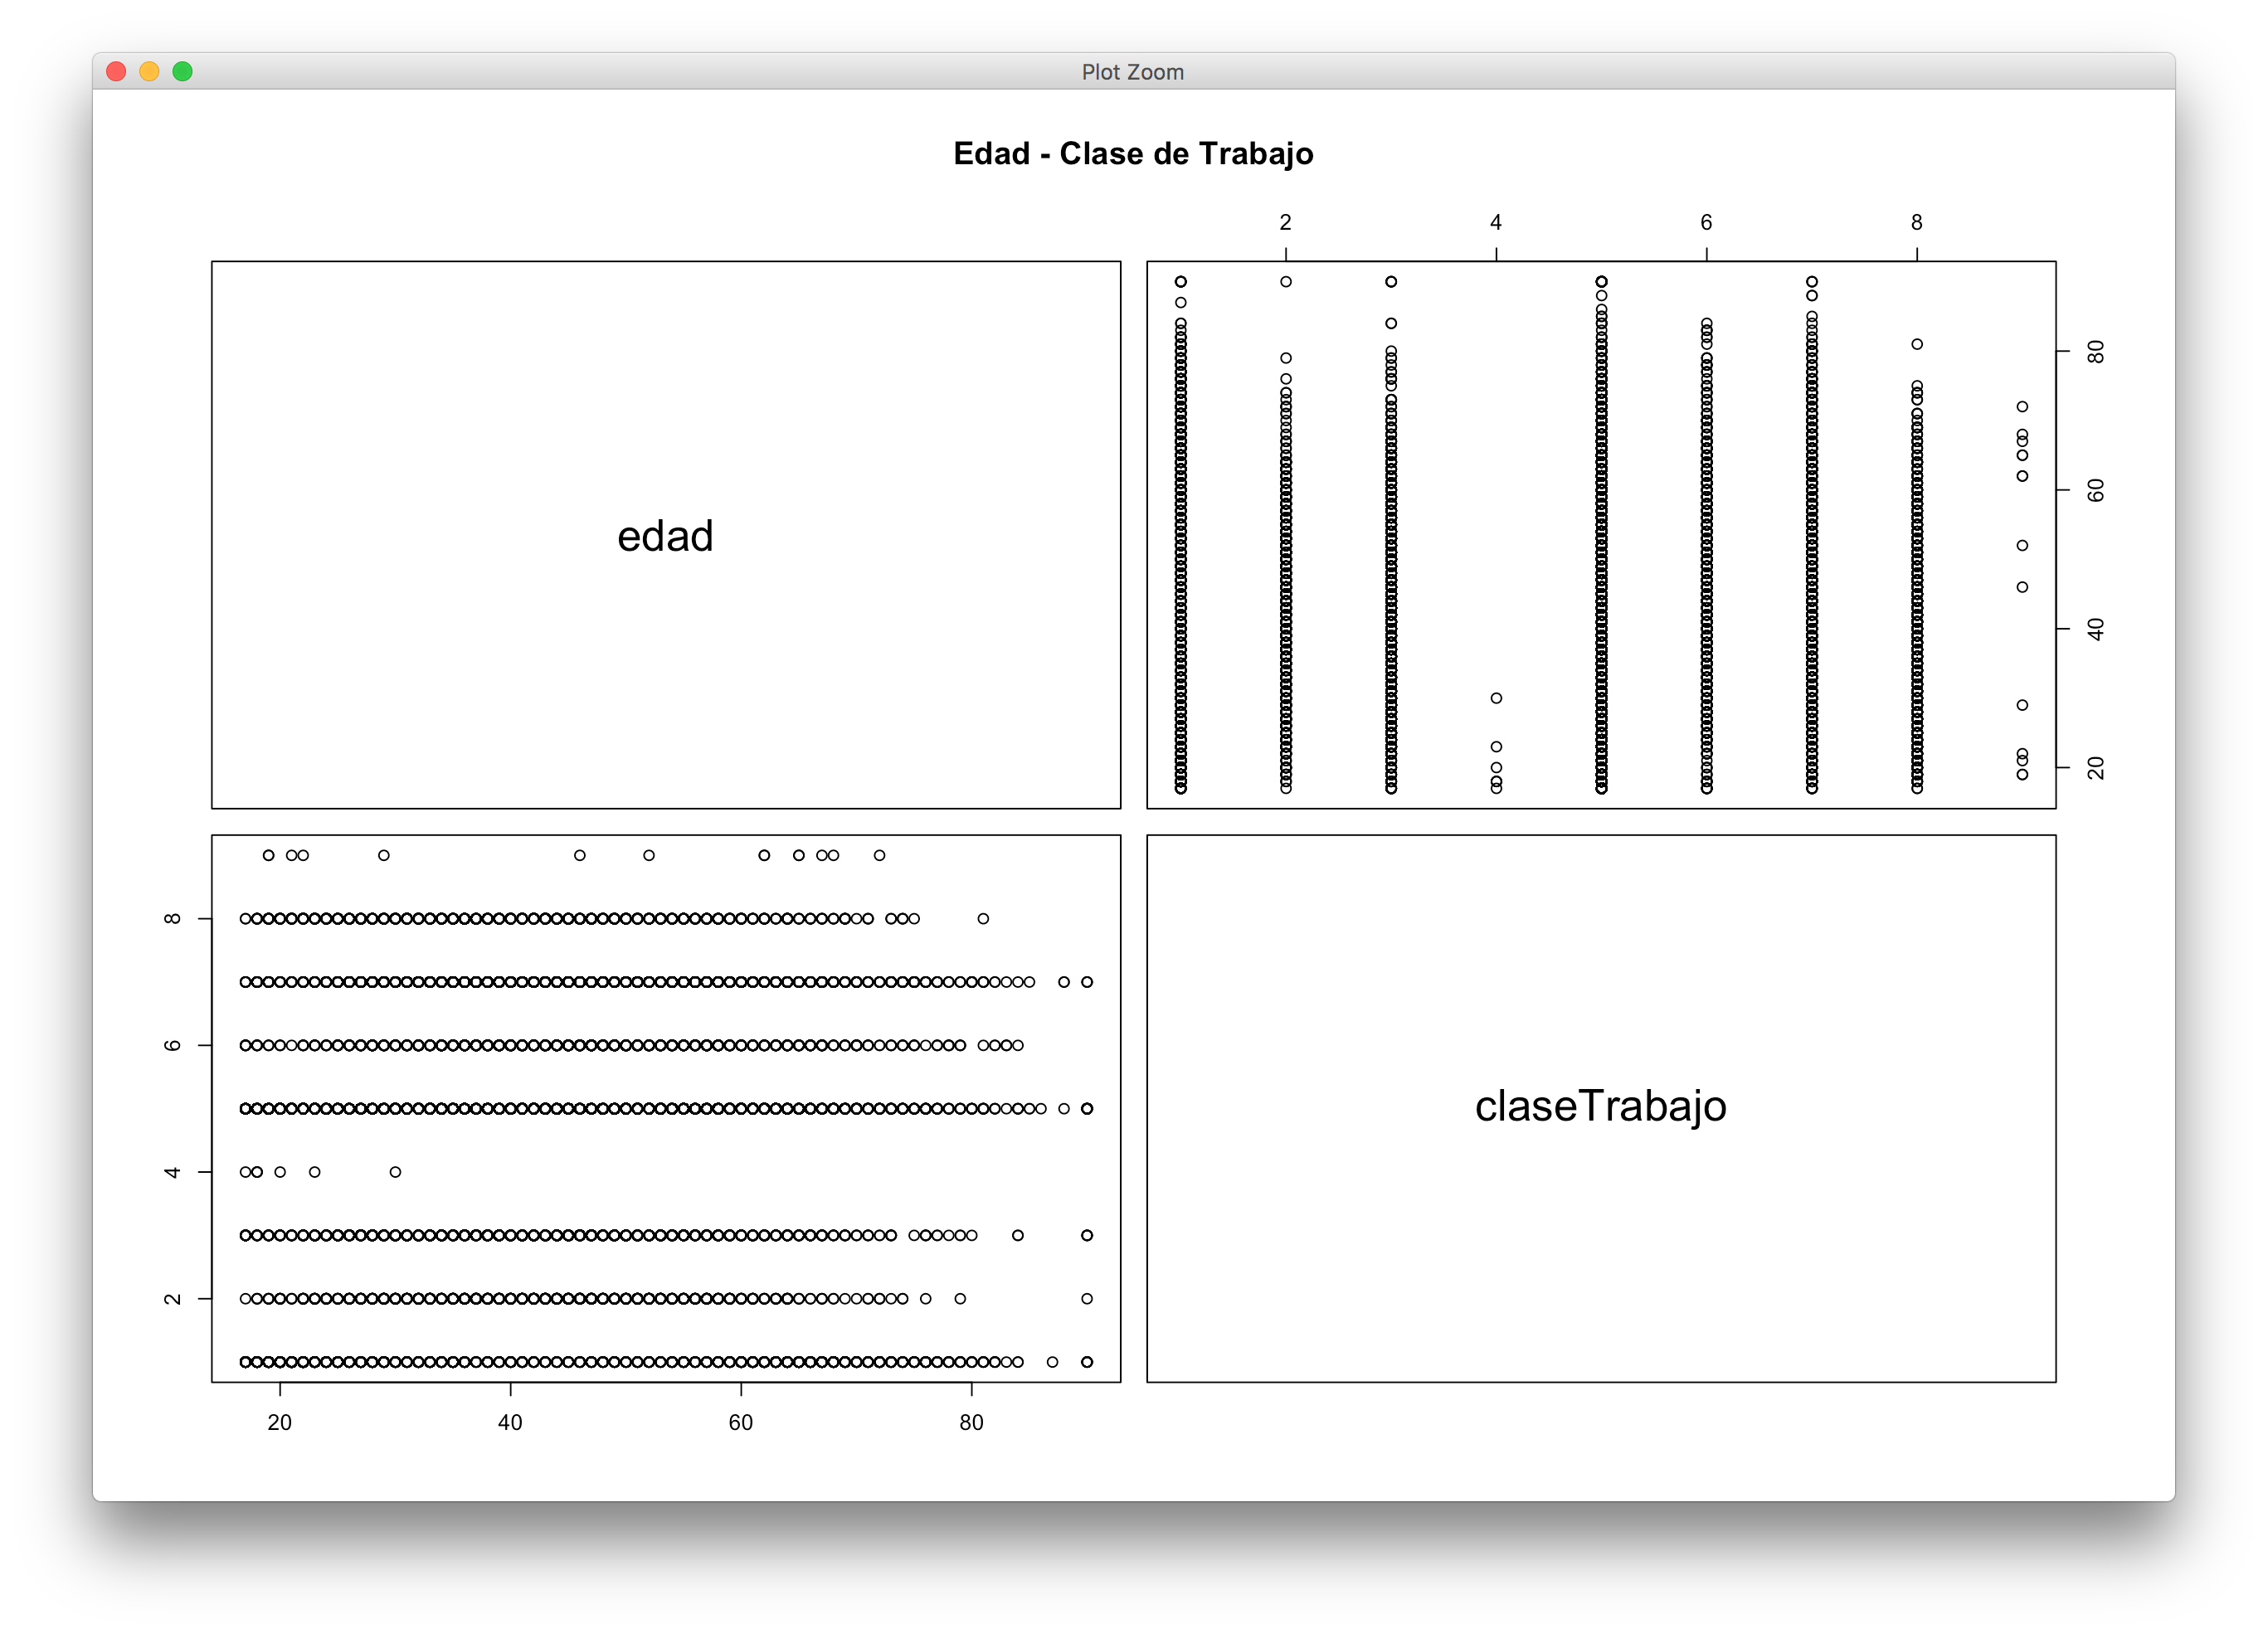
\includegraphics[scale=0.45]{graficas/edadClaseTrab}}
  \end{center}
  \begin{center}
    \hbox{\hspace{-5.5em}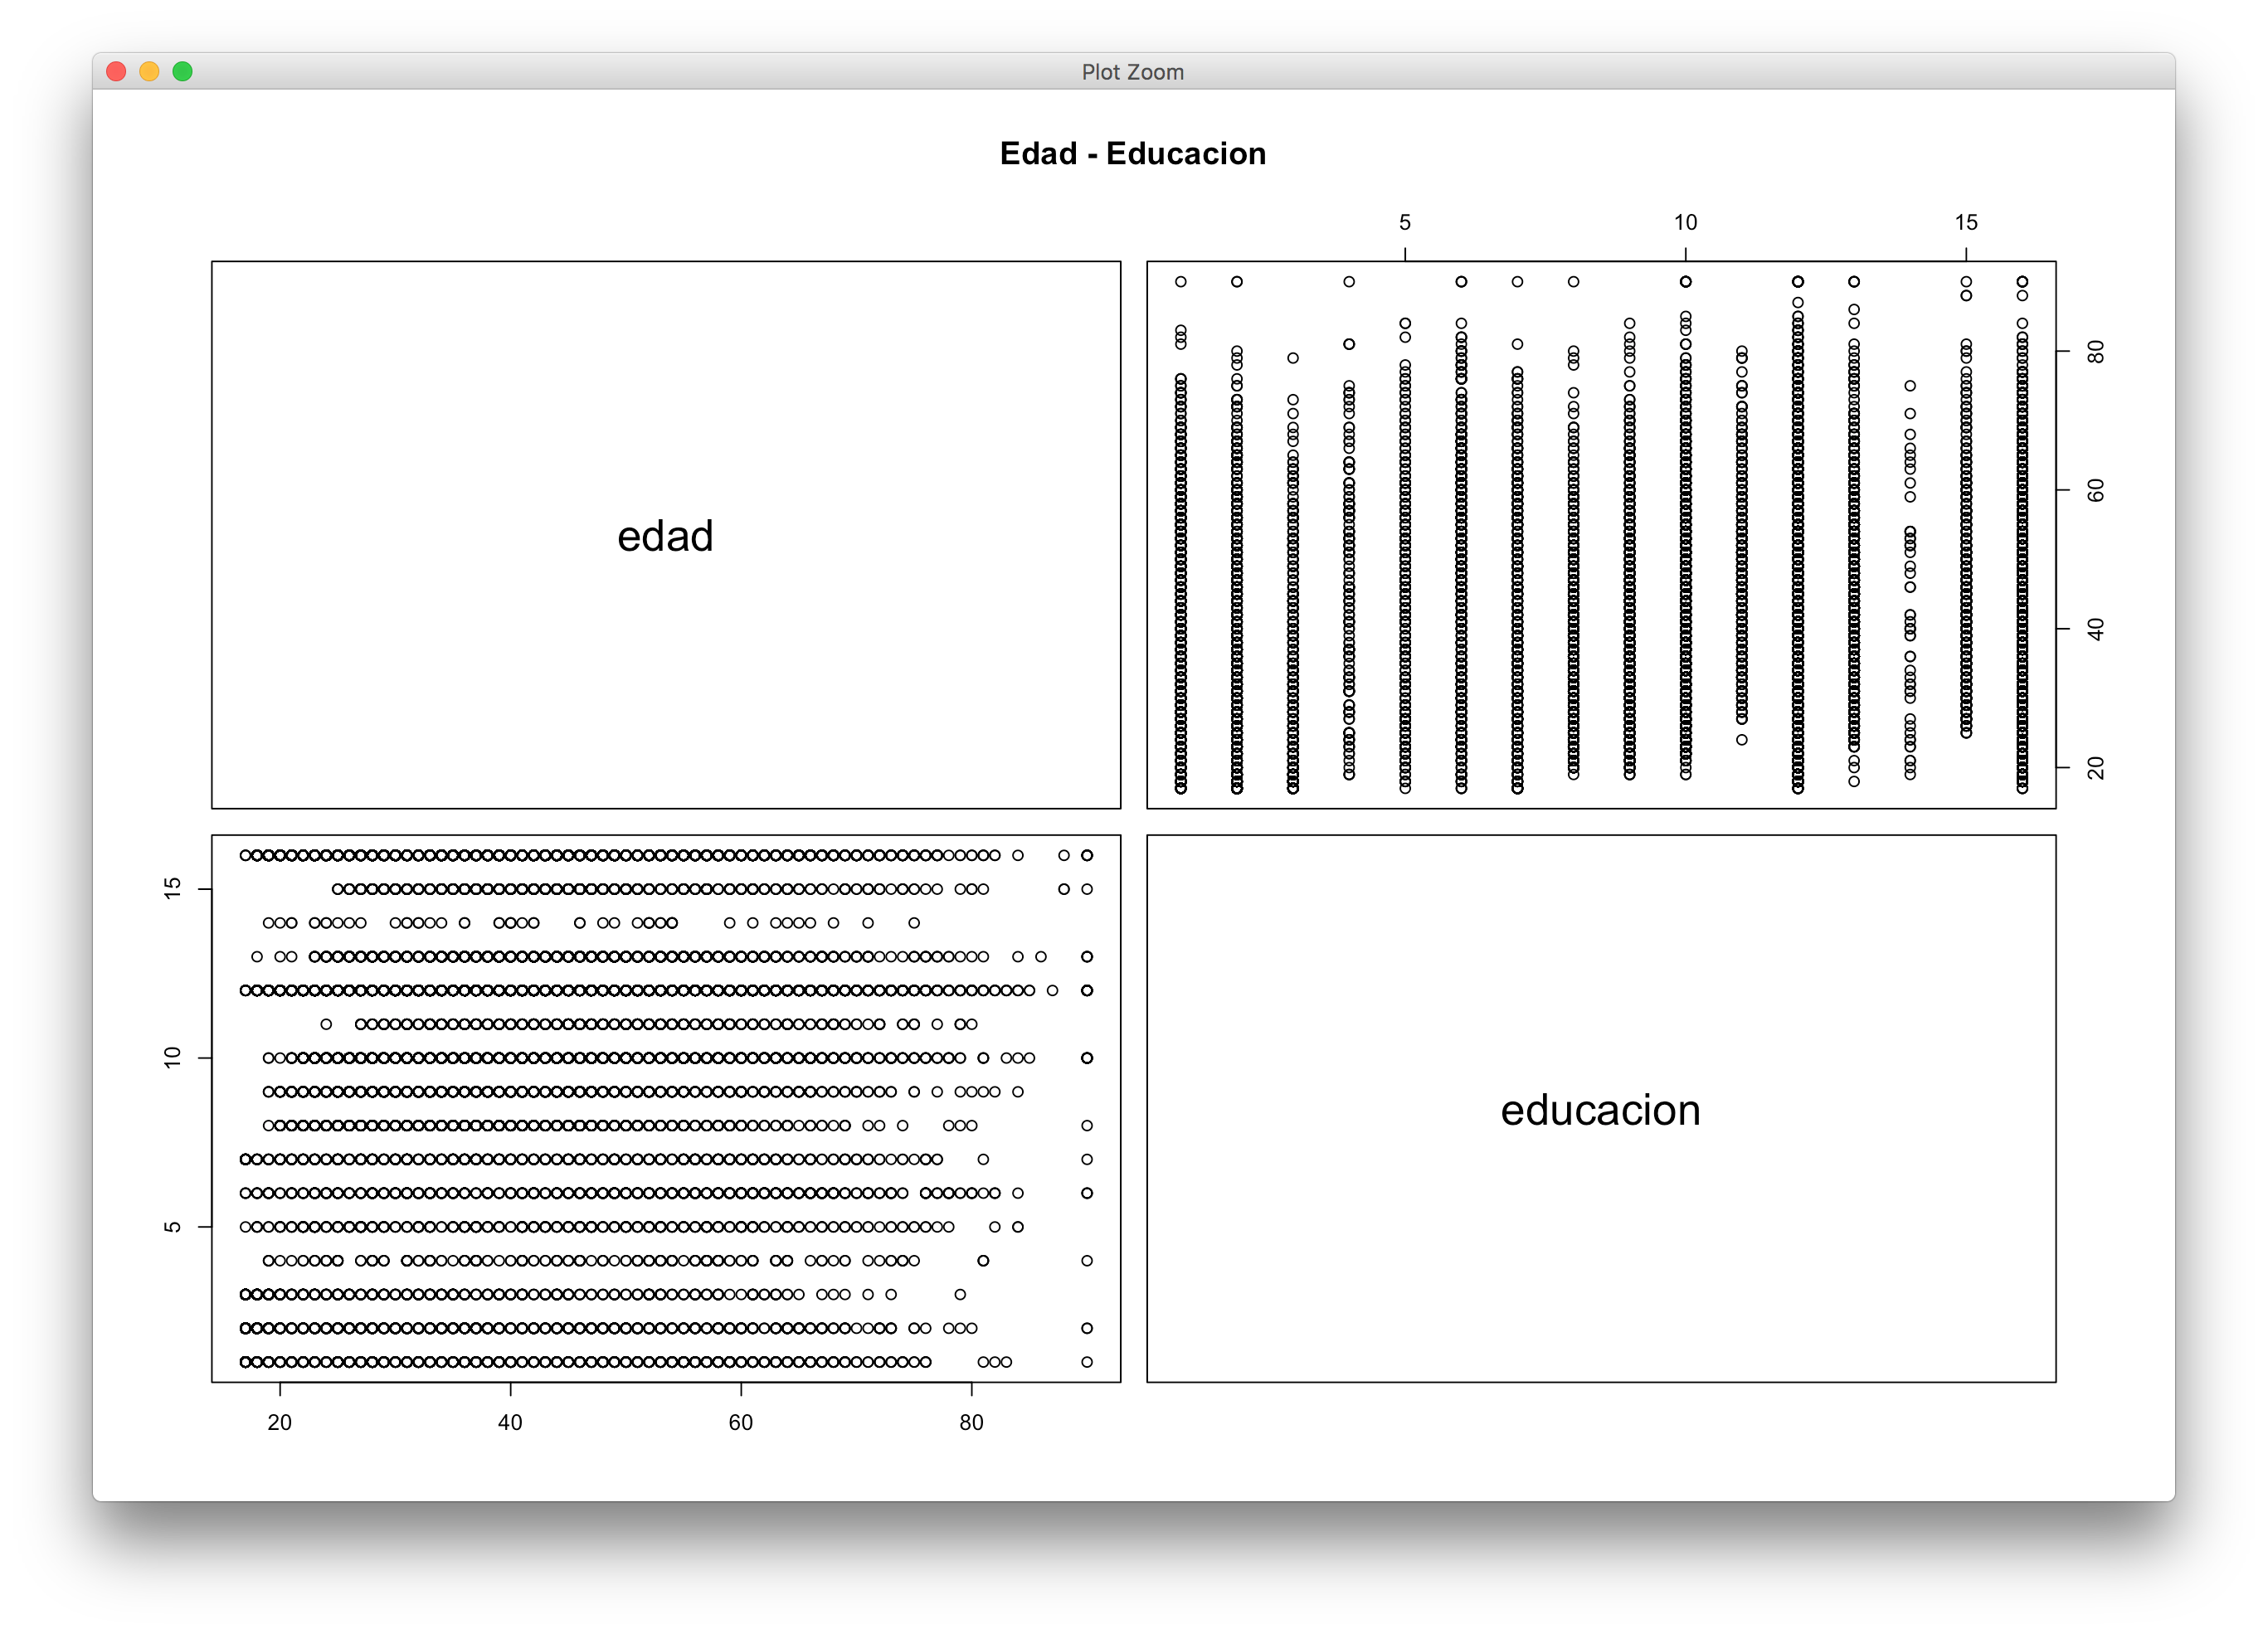
\includegraphics[scale=0.45]{graficas/edadEdu}}
  \end{center}

  \begin{center}
    \hbox{\hspace{-5.5em}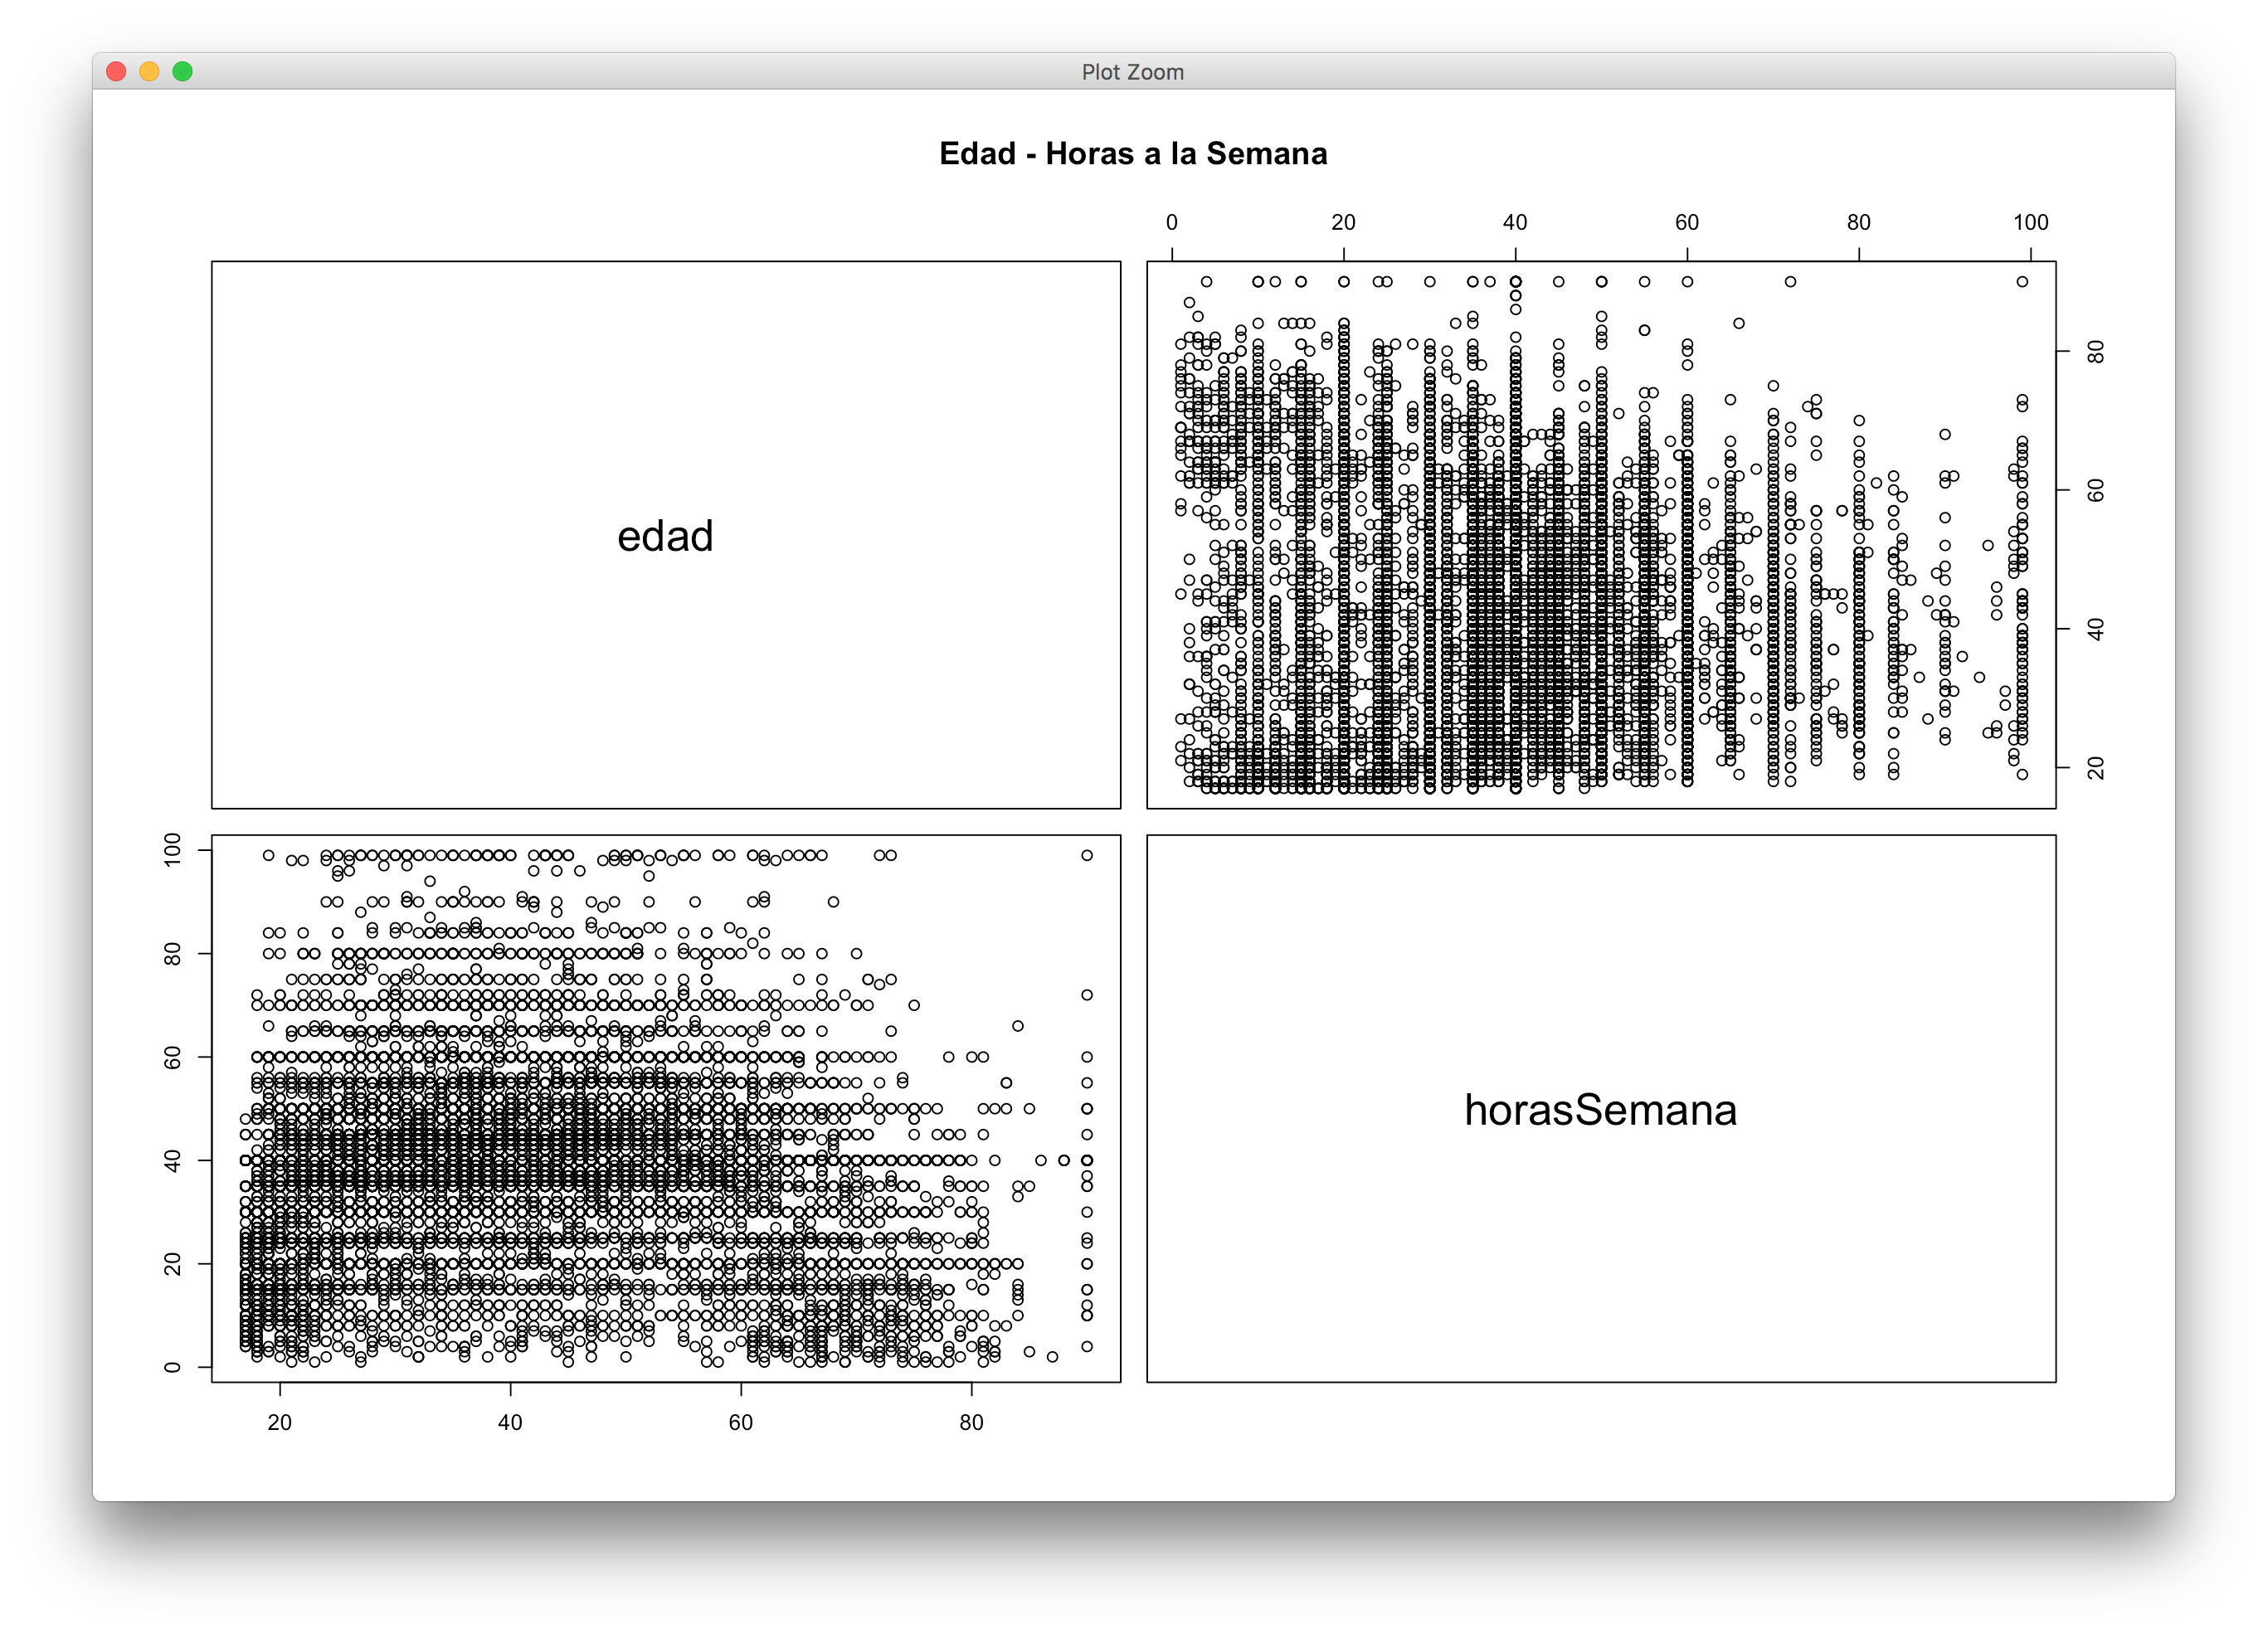
\includegraphics[scale=0.45]{graficas/edadHoras}}
  \end{center}
  \begin{center}
    \hbox{\hspace{-5.5em}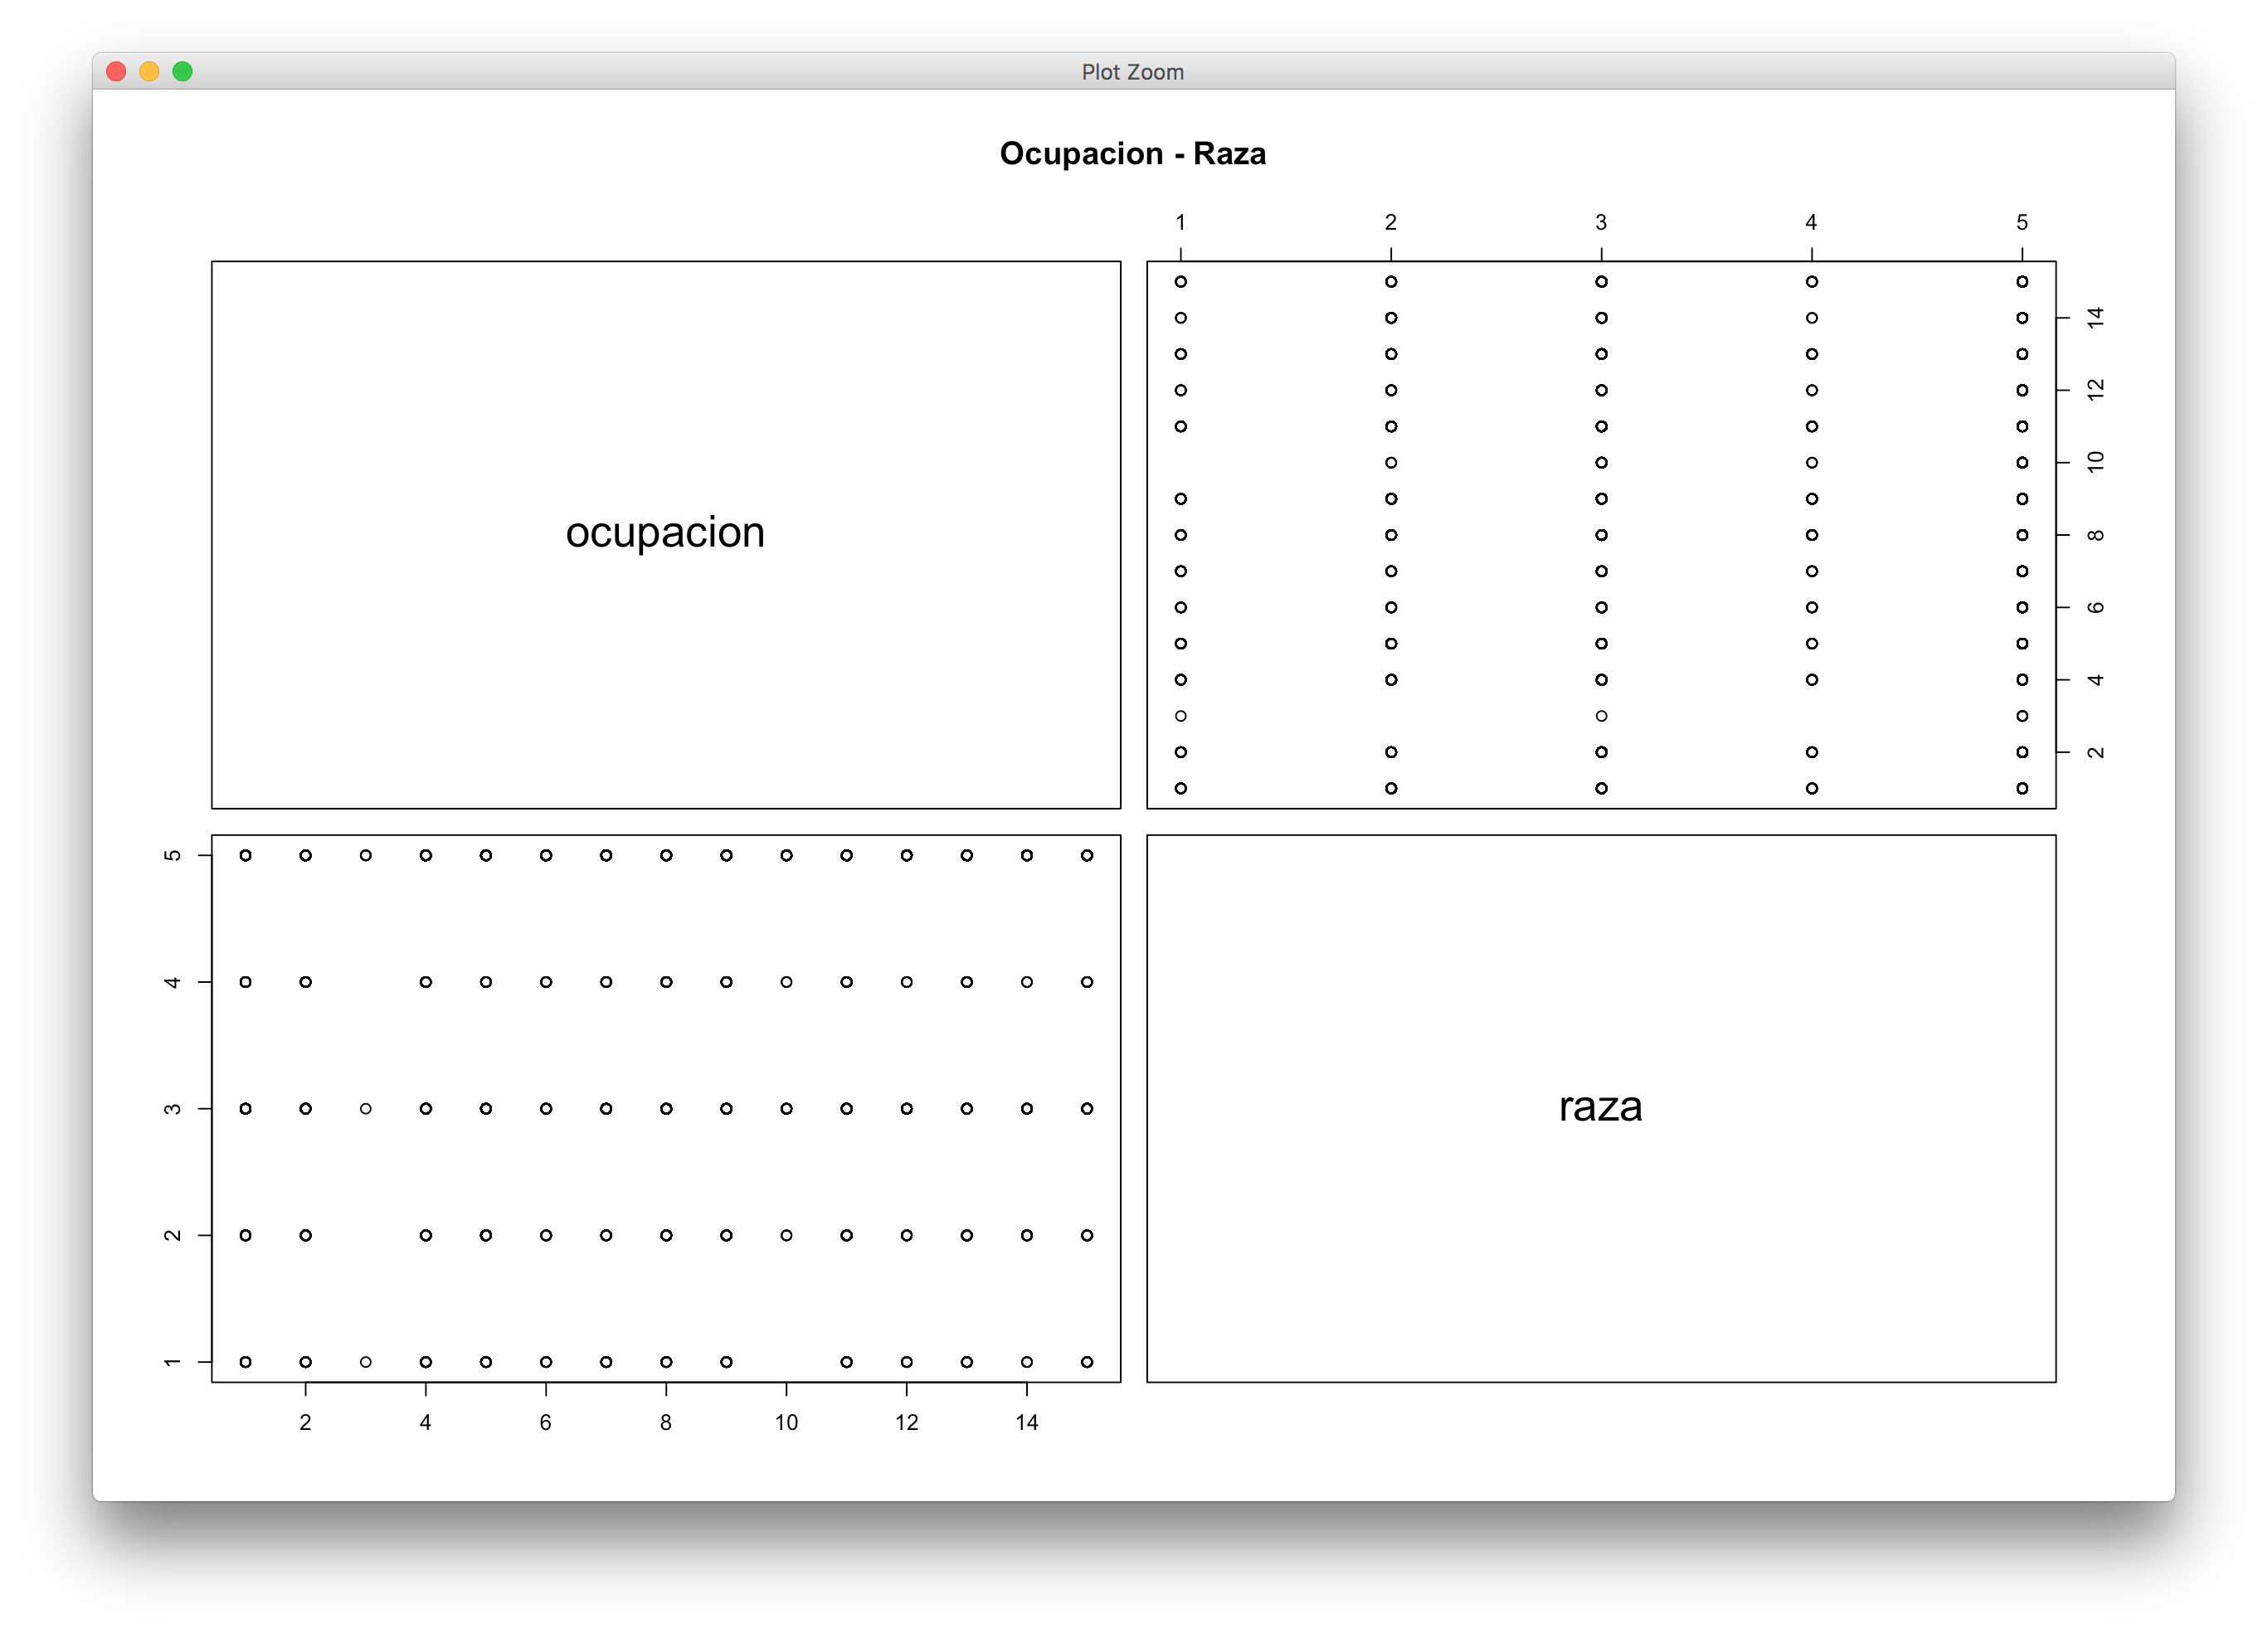
\includegraphics[scale=0.45]{graficas/ocupacion-raza}}
  \end{center}
  \begin{center}
    \hbox{\hspace{-5.5em}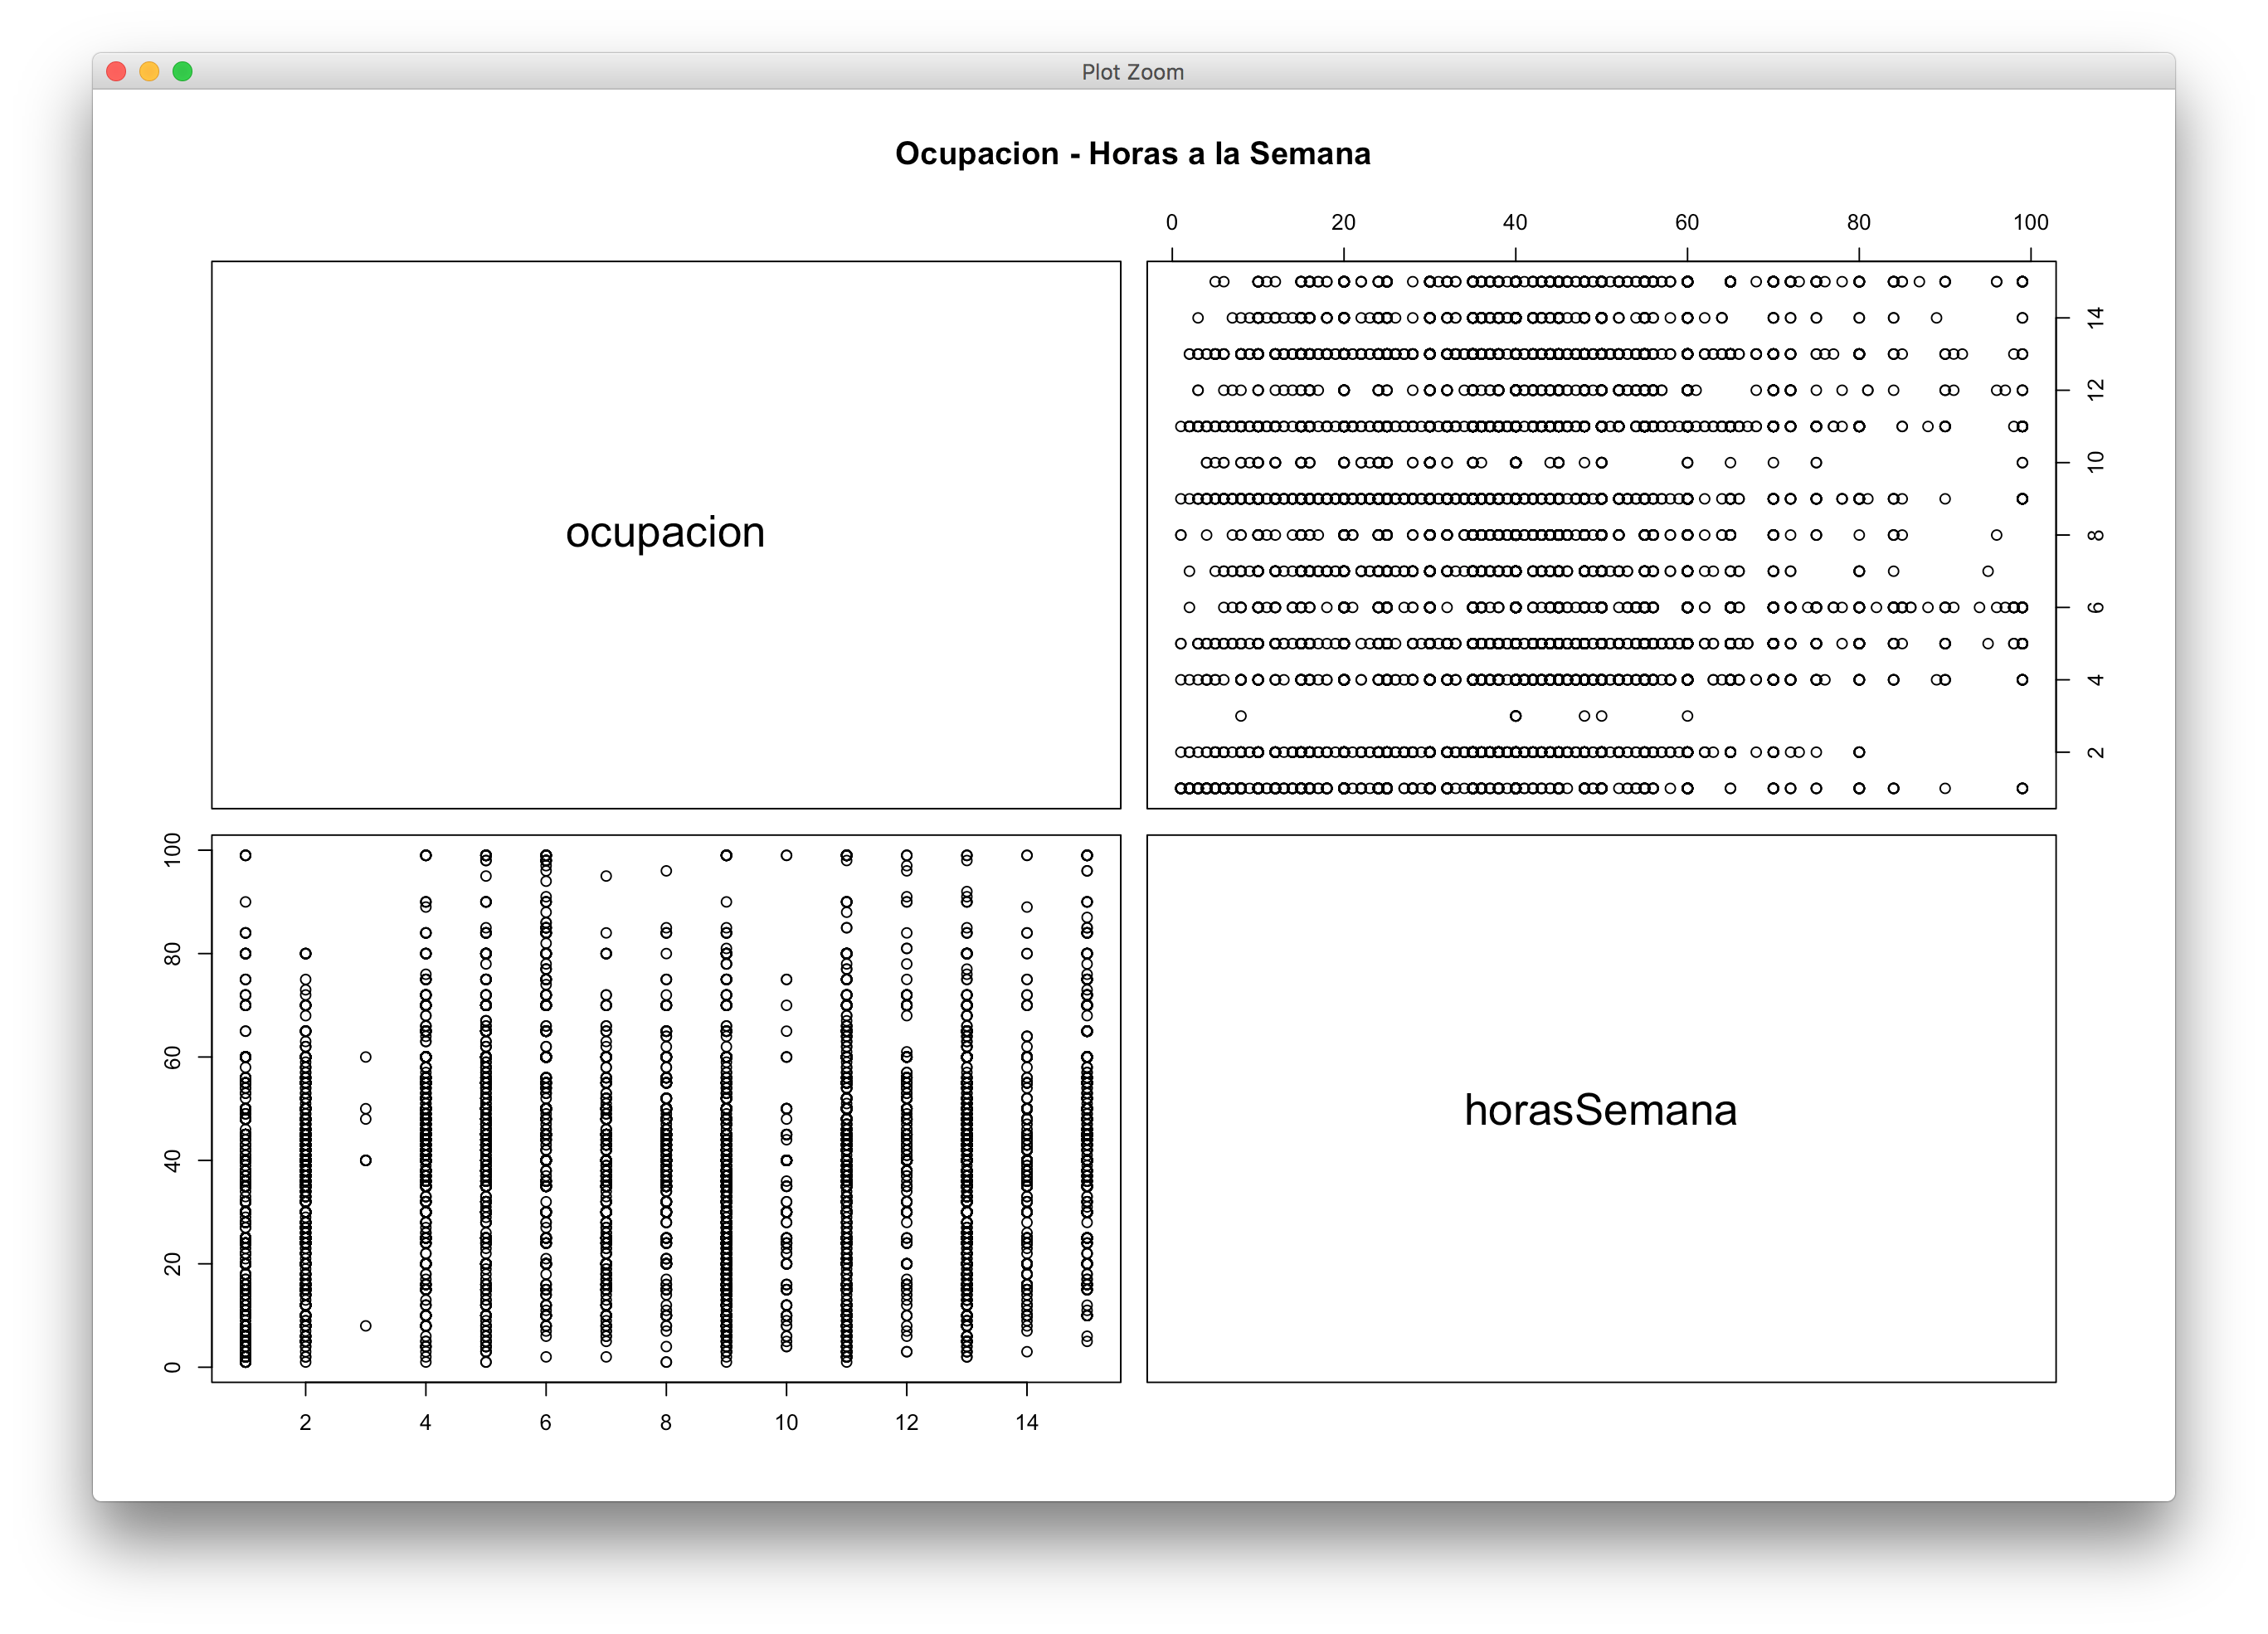
\includegraphics[scale=0.45]{graficas/ocupacionHoras}}
  \end{center}
  \begin{center}
    \hbox{\hspace{-5.5em}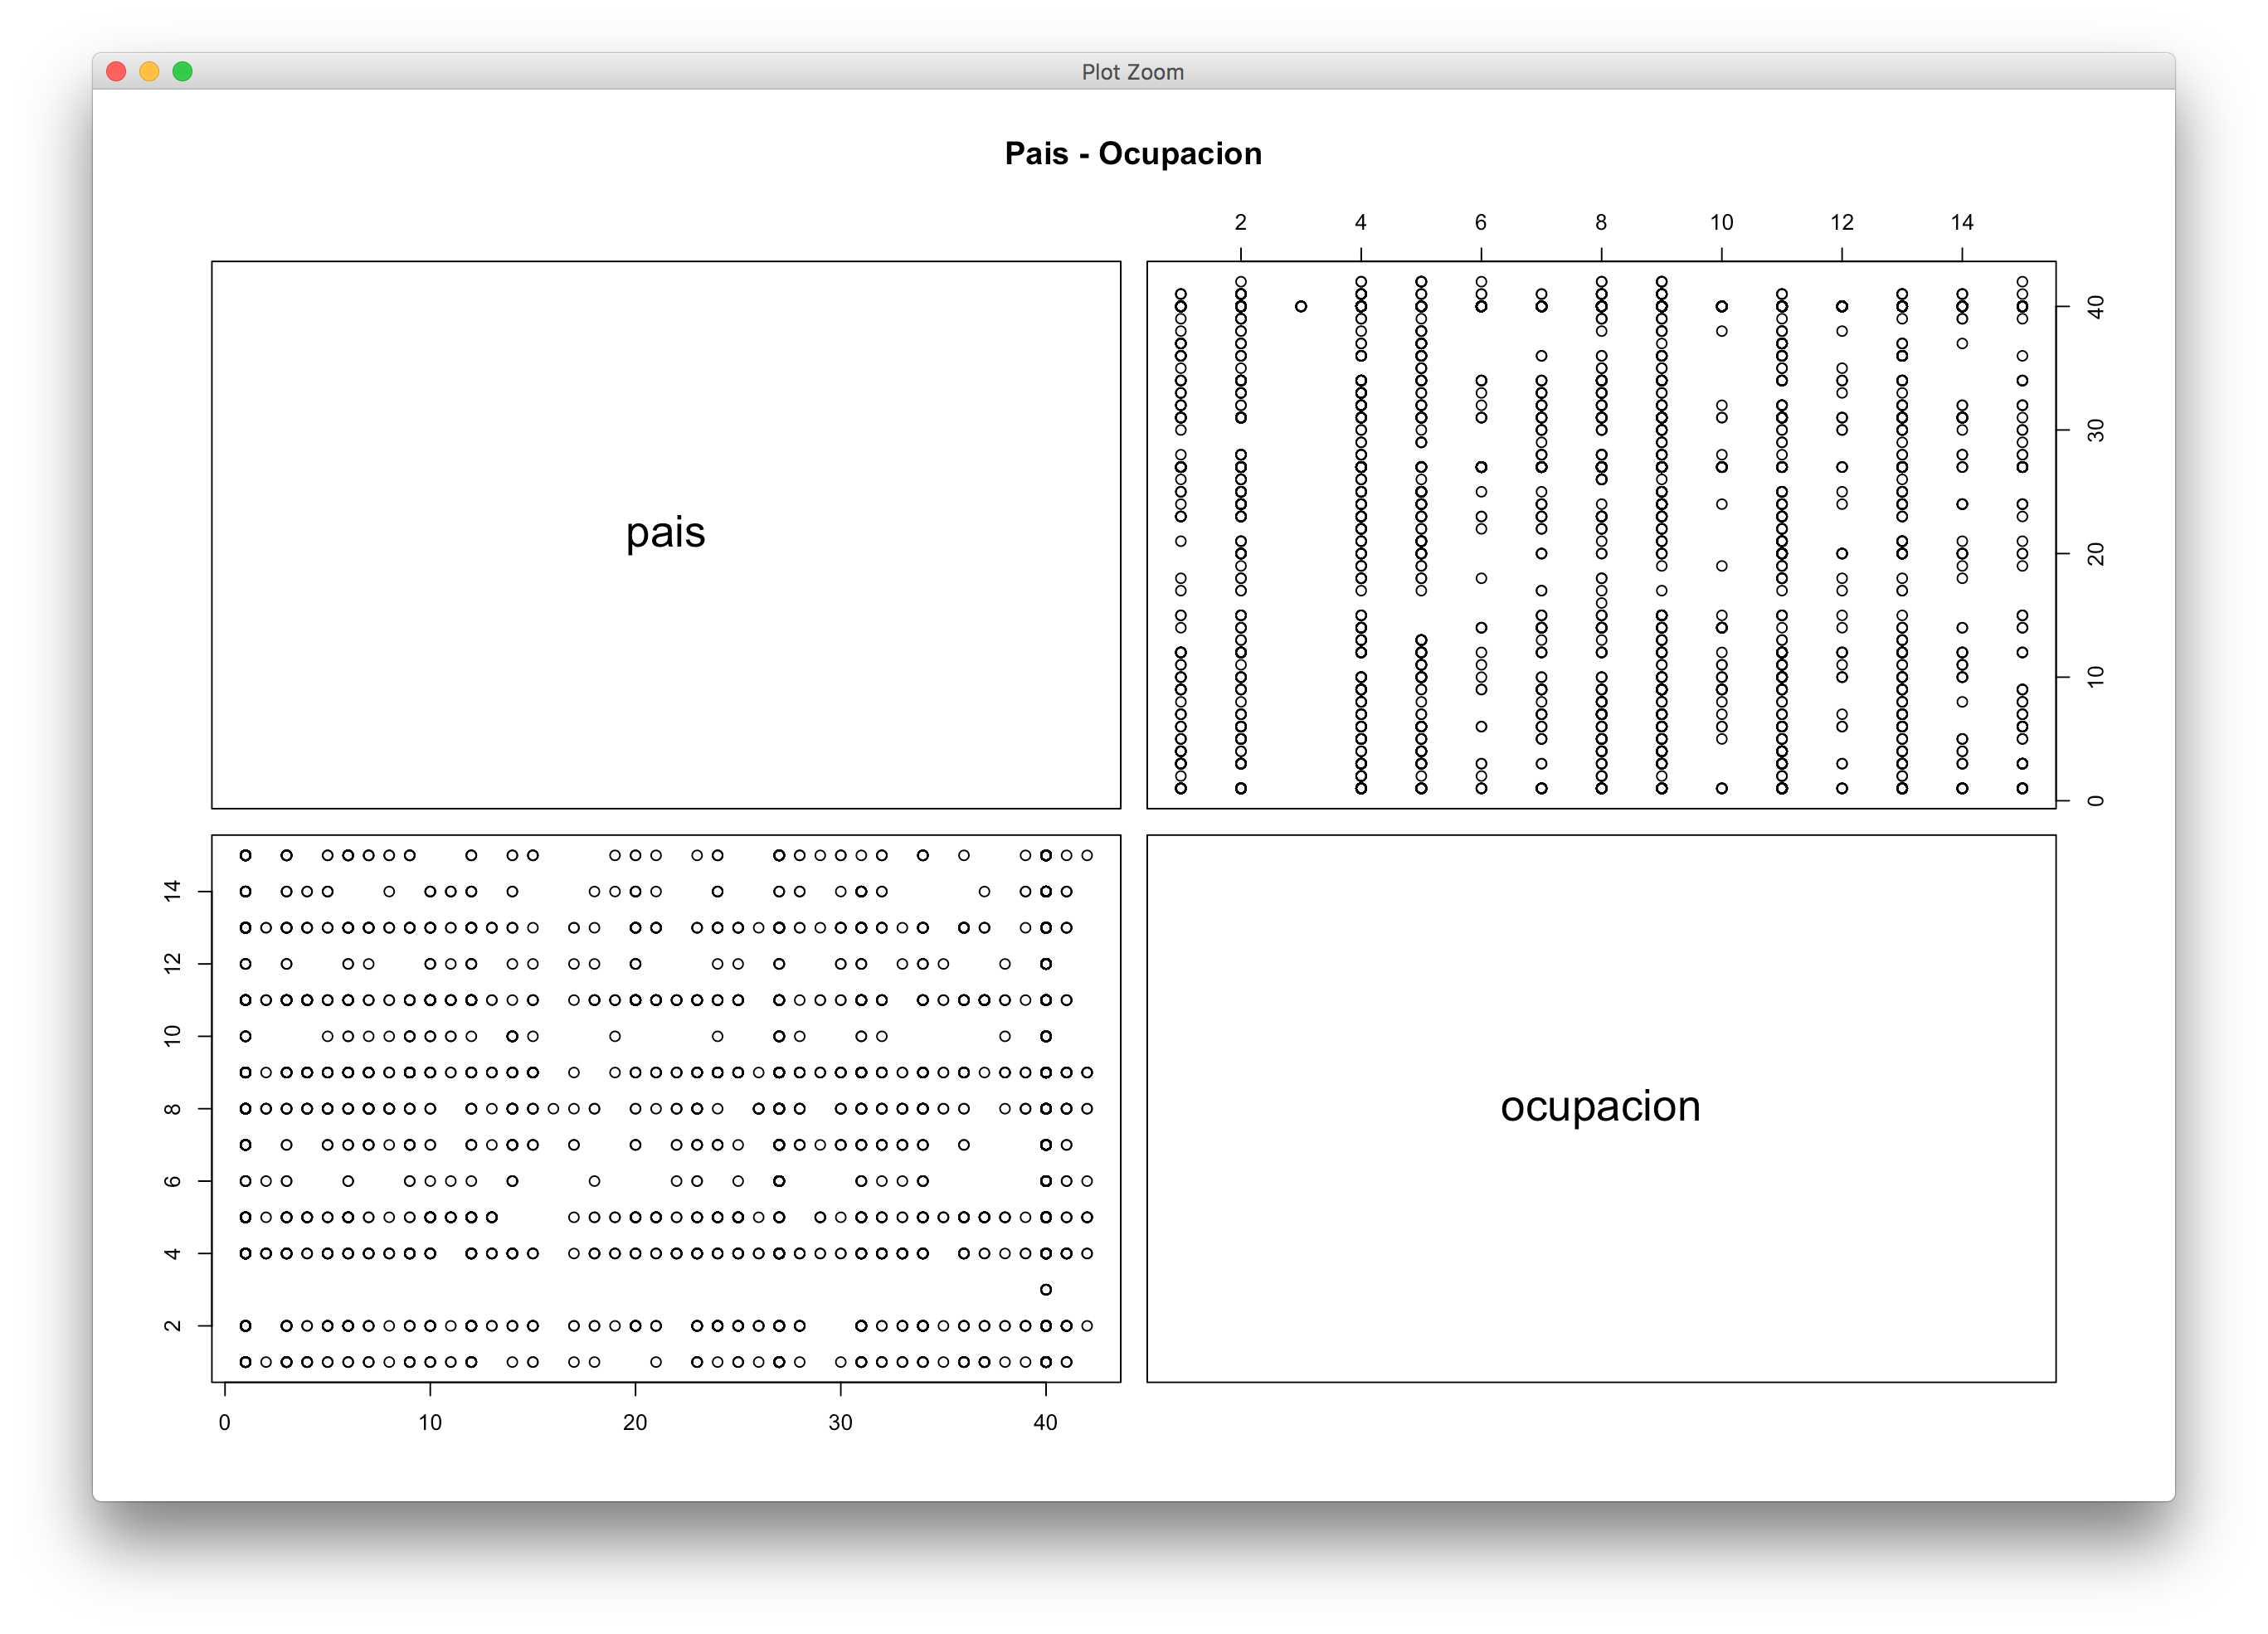
\includegraphics[scale=0.45]{graficas/pais-ocupacion}}
  \end{center}
  \begin{center}
    \hbox{\hspace{-5.5em}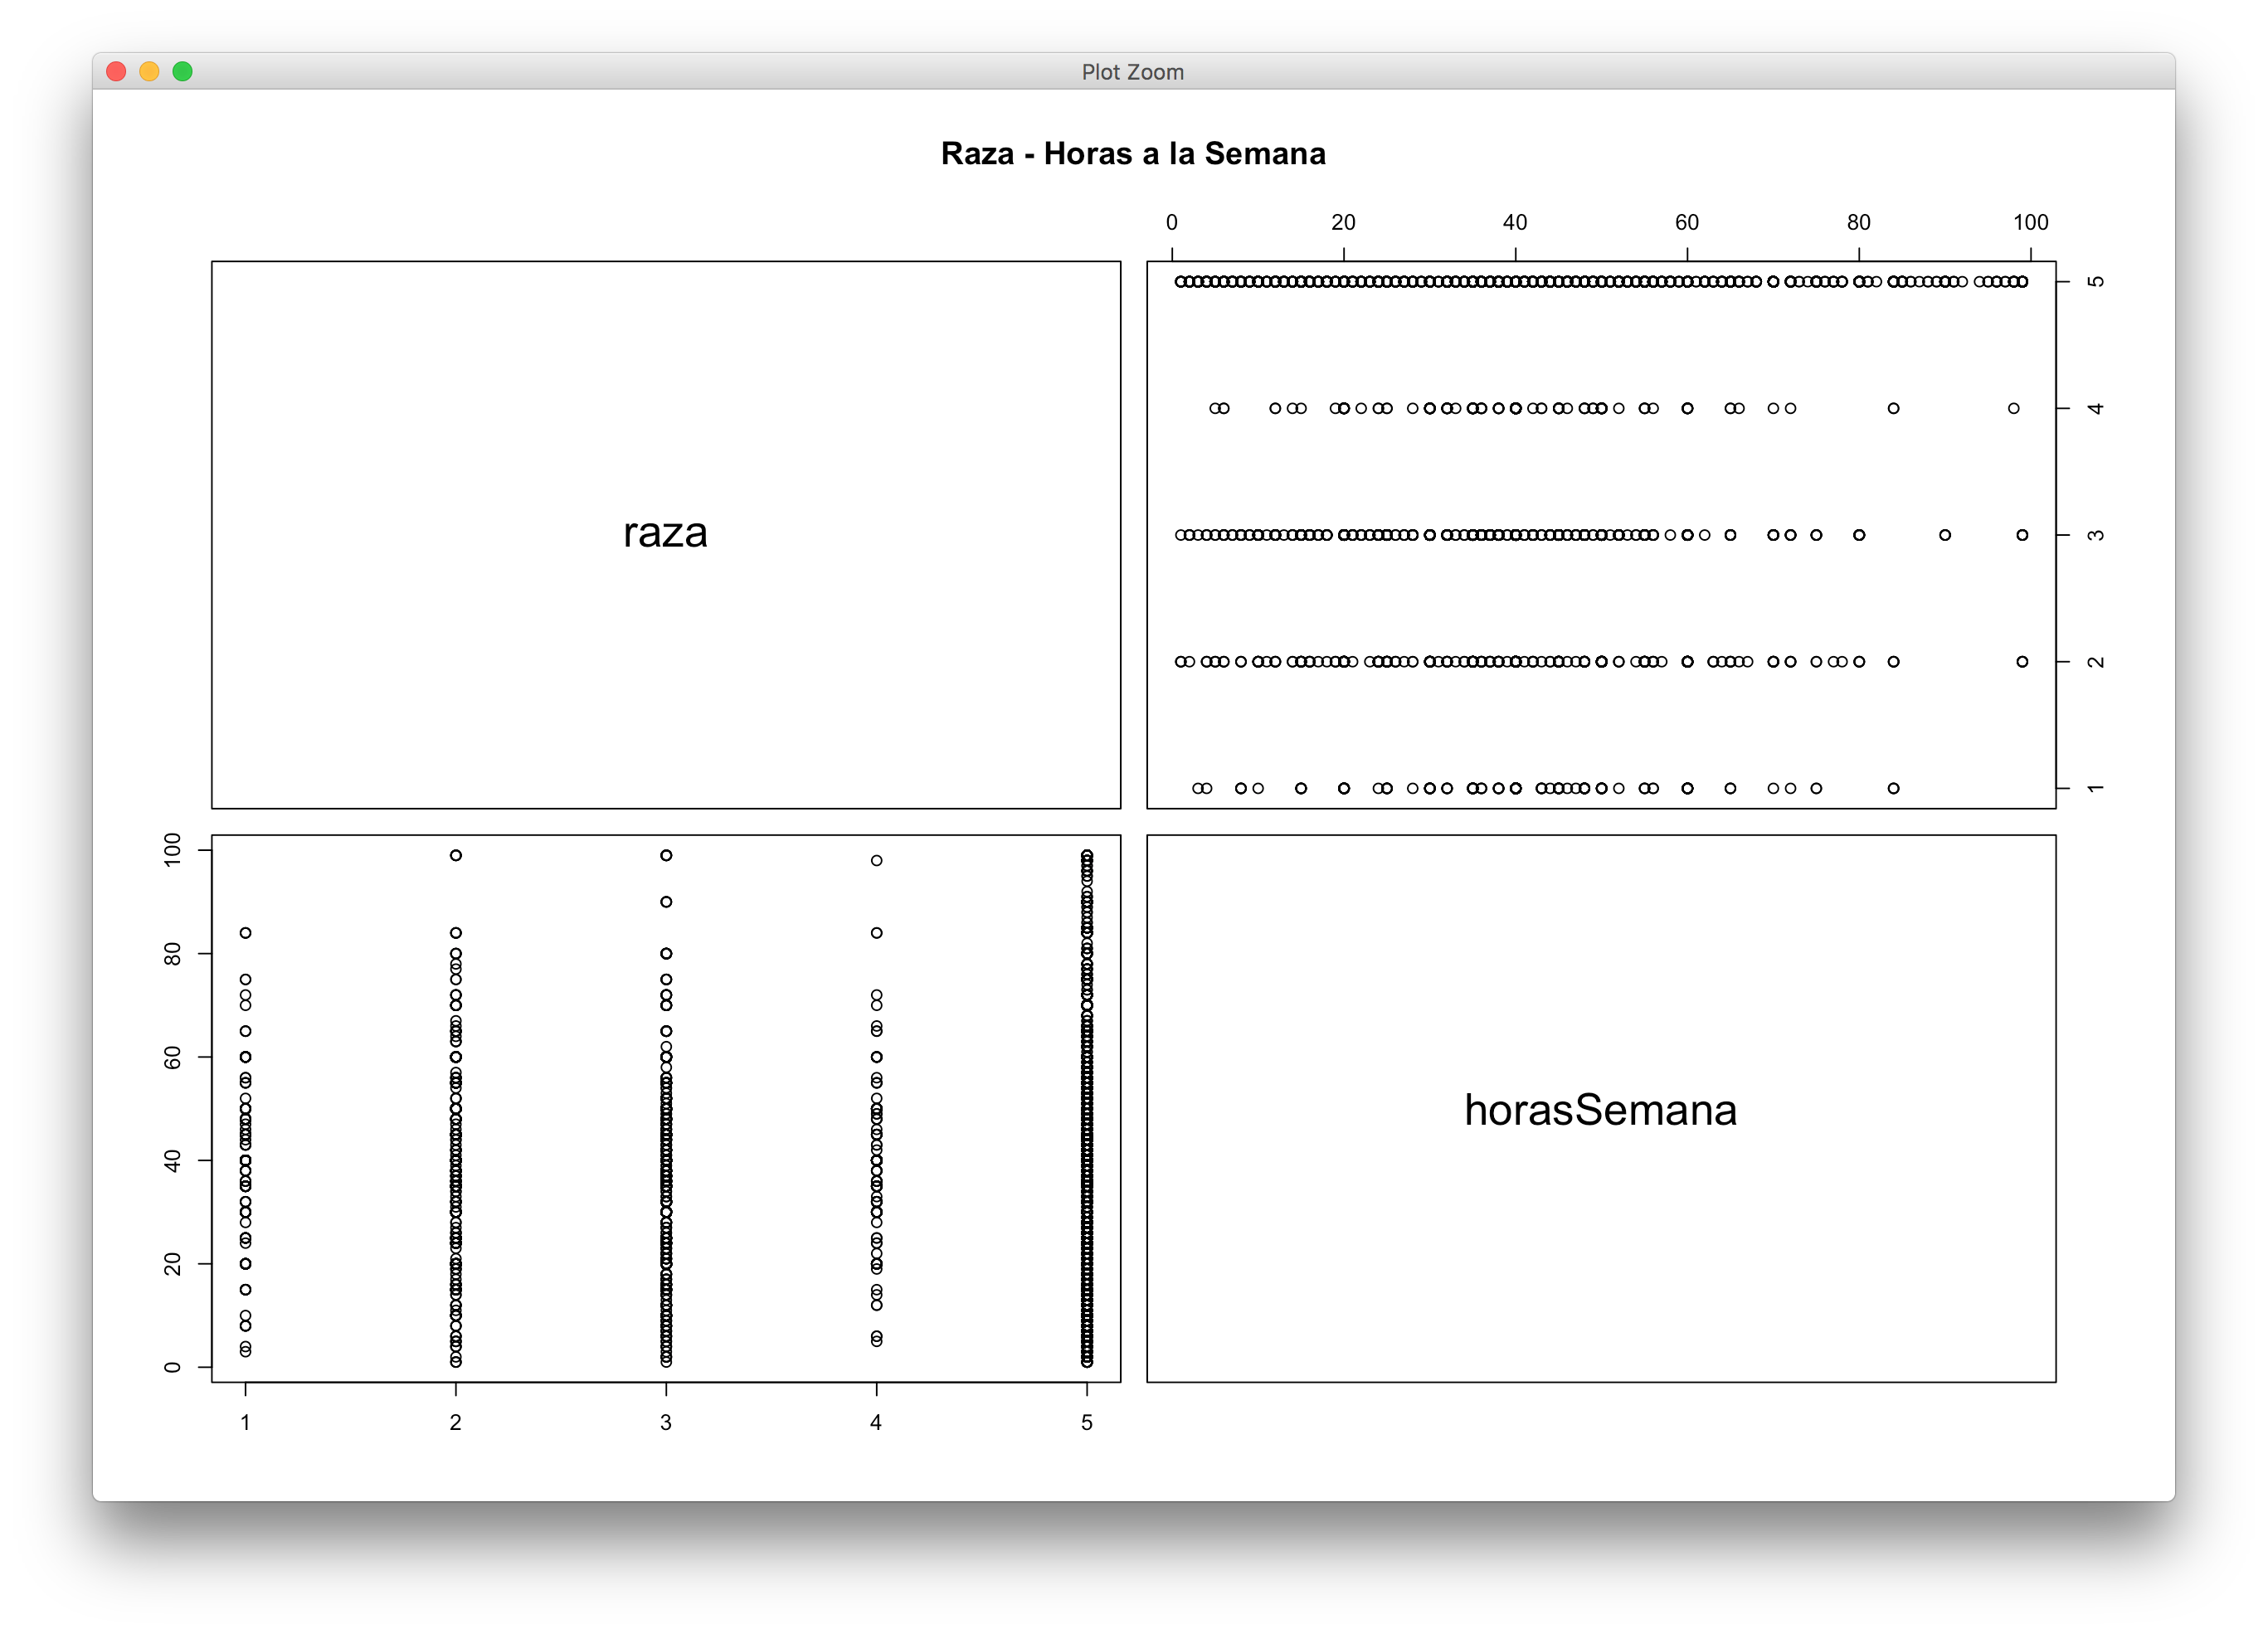
\includegraphics[scale=0.45]{graficas/raza-horas}}
  \end{center}
  \begin{center}
    \hbox{\hspace{-5.5em}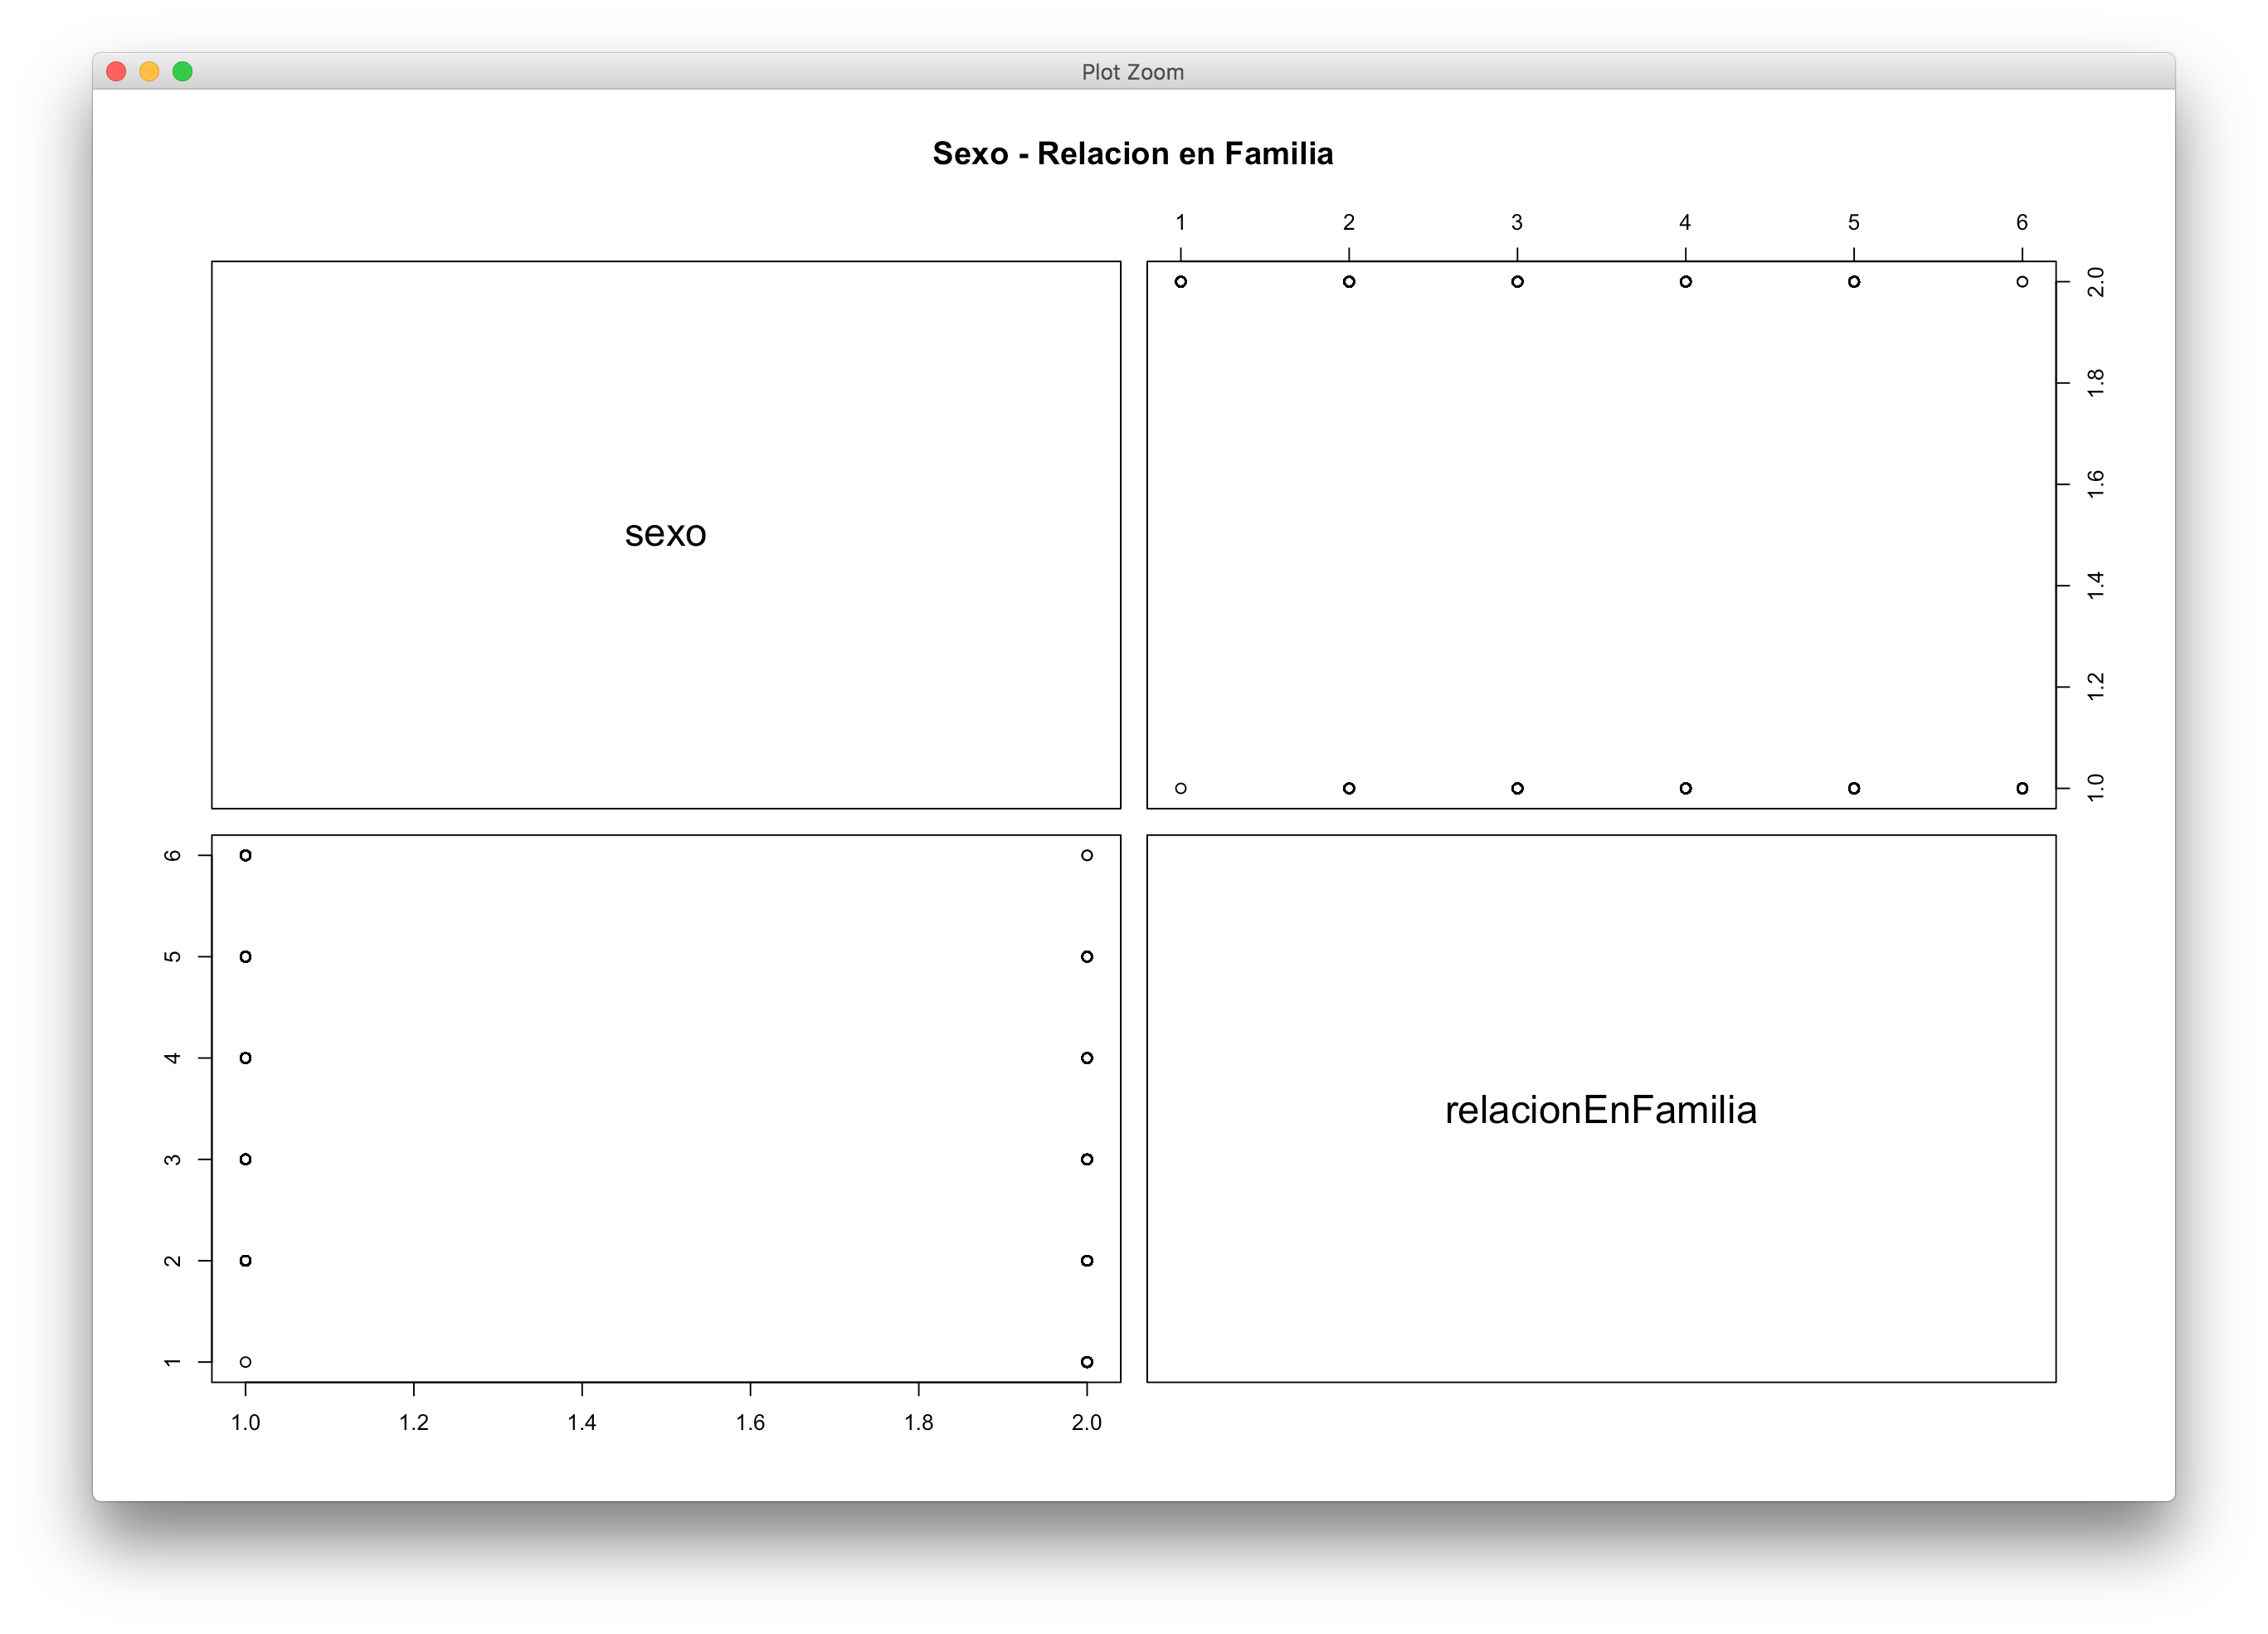
\includegraphics[scale=0.45]{graficas/Sexo-RelFam}}
  \end{center}
\section{Preprocesamiento}
  Lo primero que haremos es eliminar al atributo {\it education\_num}, despues generaremos las tablas de frecuencias de cada atributo, estas se pueden encontrar en el archivo {\it preprocesamiento.sql}. Solo faltaria graficar las tablas obtenidas
  \begin{center}
    \hbox{\hspace{-5.5em}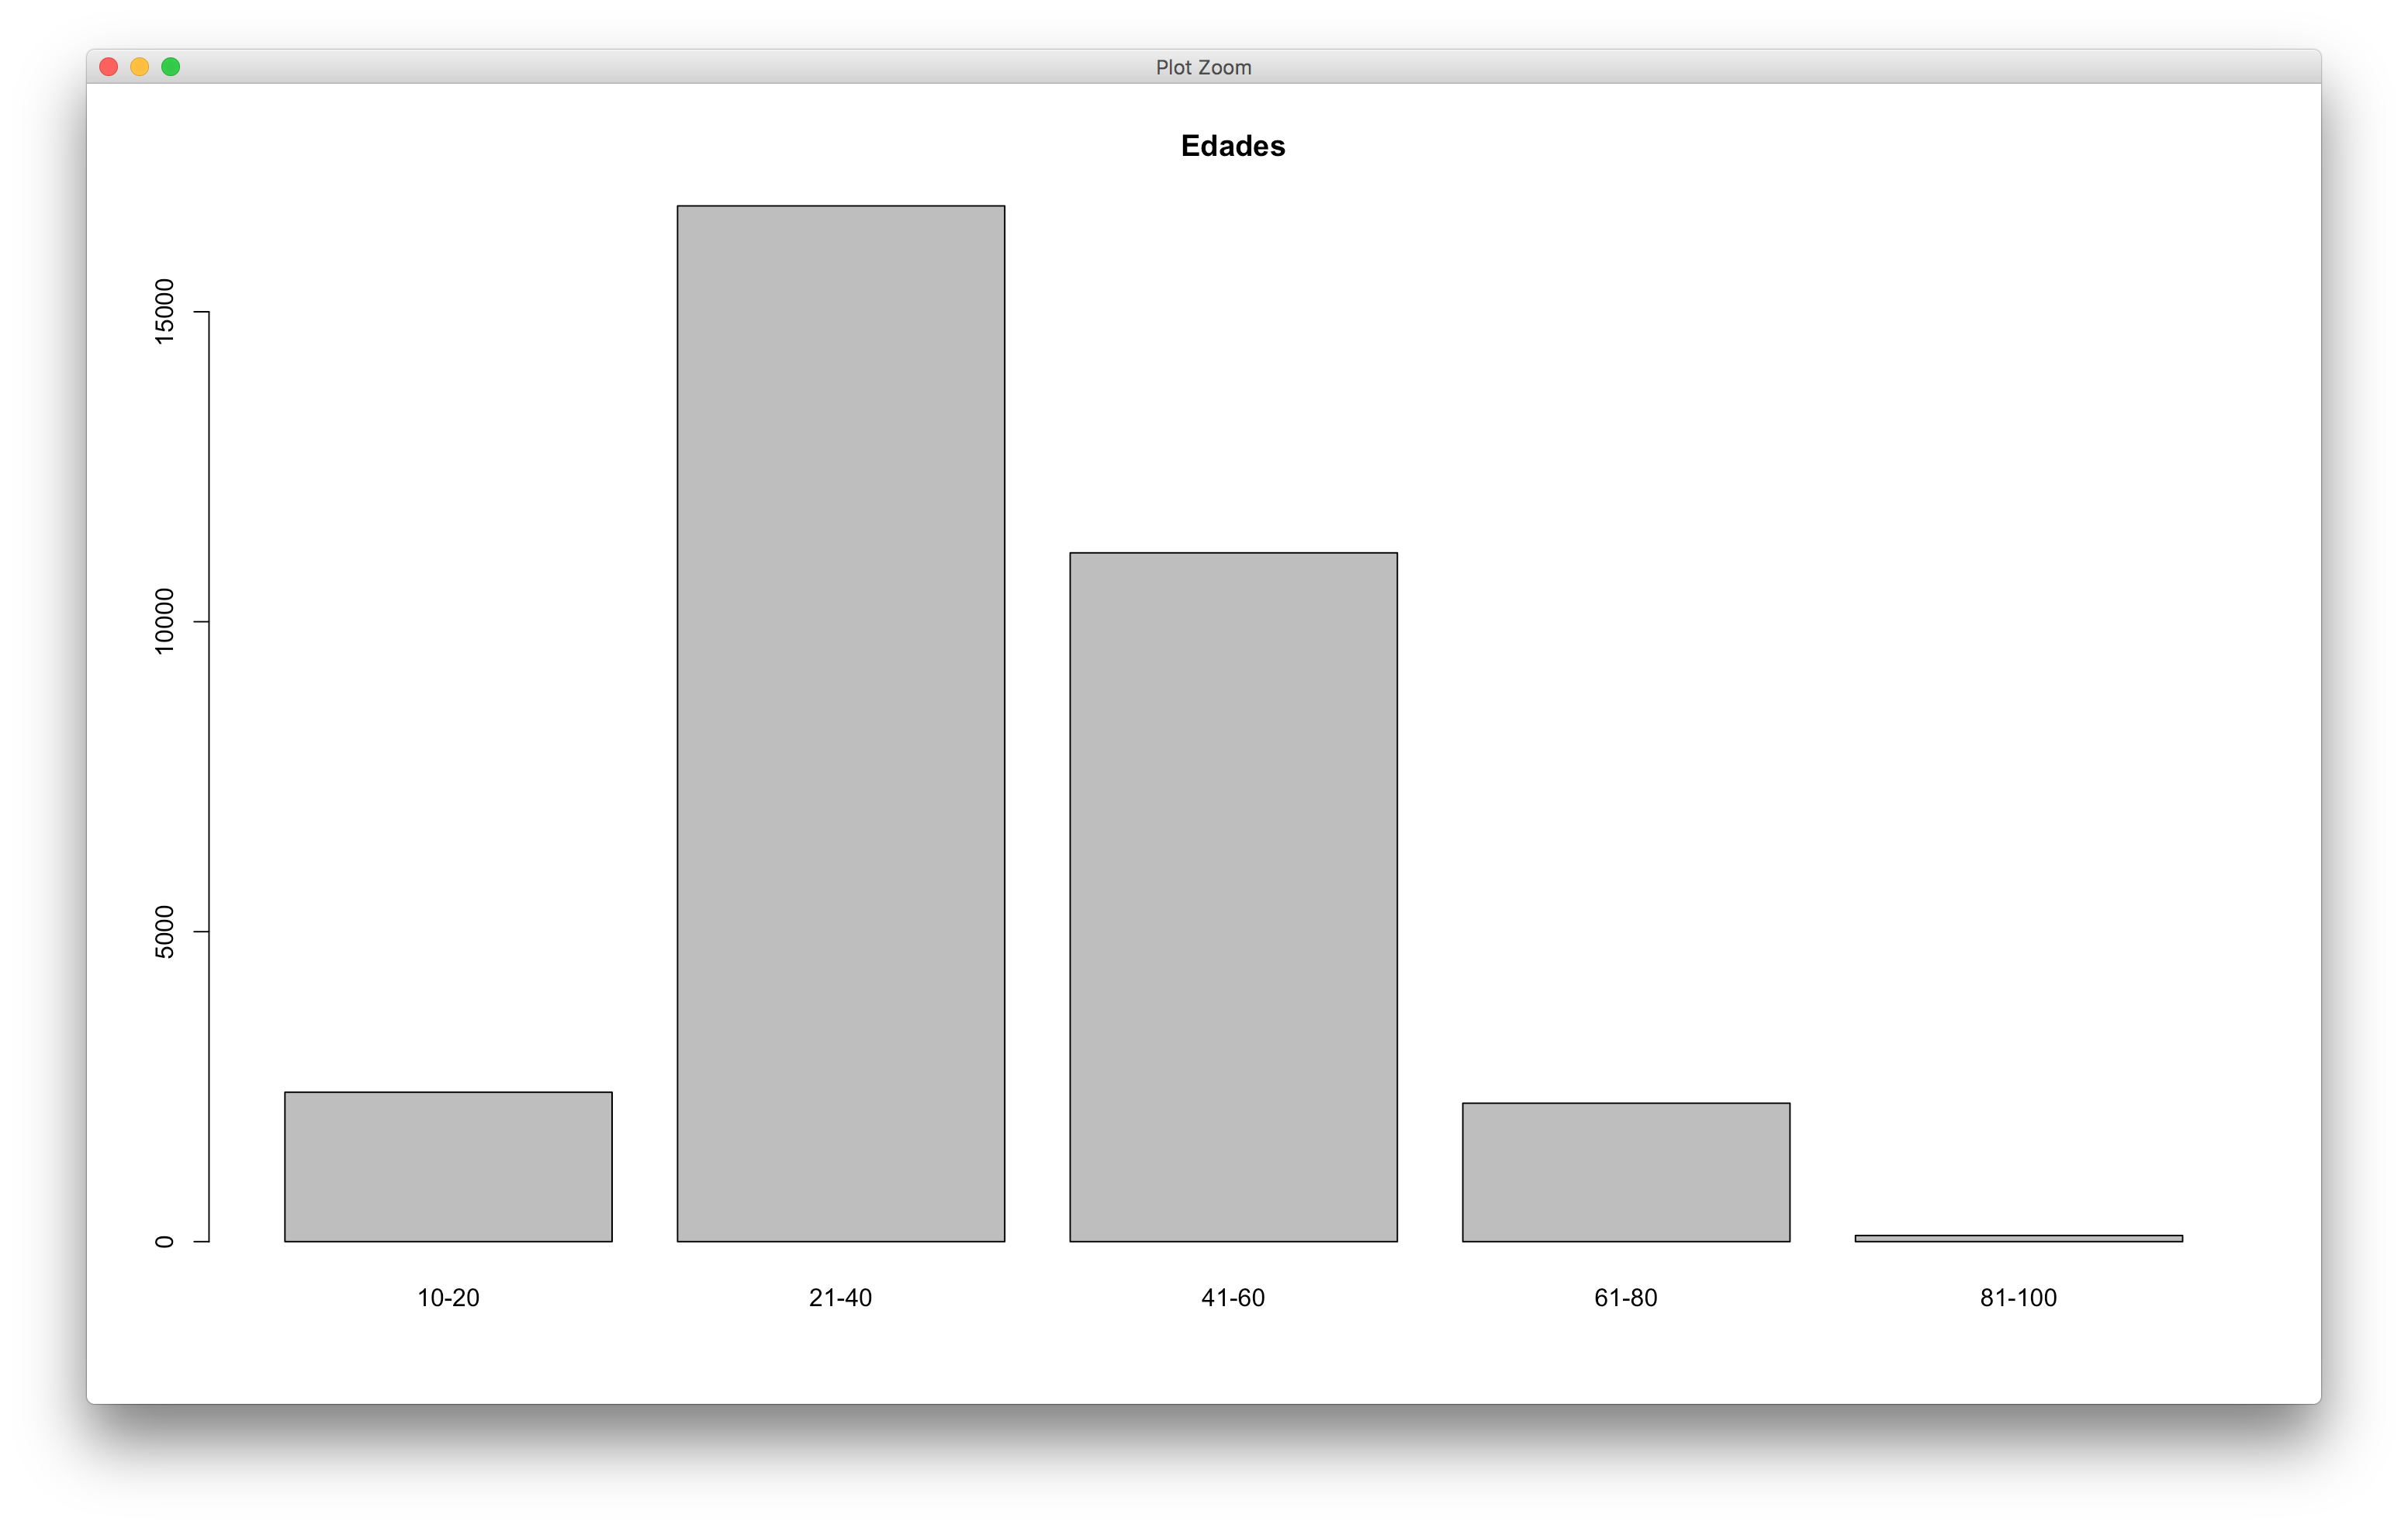
\includegraphics[scale=0.4]{graficas/edadesP}}
  \end{center}
  En esta gráfica podemos observar que el rango mas alto es de 21 a 40 años mientras que el menor es de 81 a 100 años, también el otro que se repute bastante son las edades que están en tres 41 y 60 años, entonces podríamos decir que en general las personas de nuestro conjunto de datos se encuentran en el rango de 21 a 60 años.
  \begin{center}
    \hbox{\hspace{-5.5em}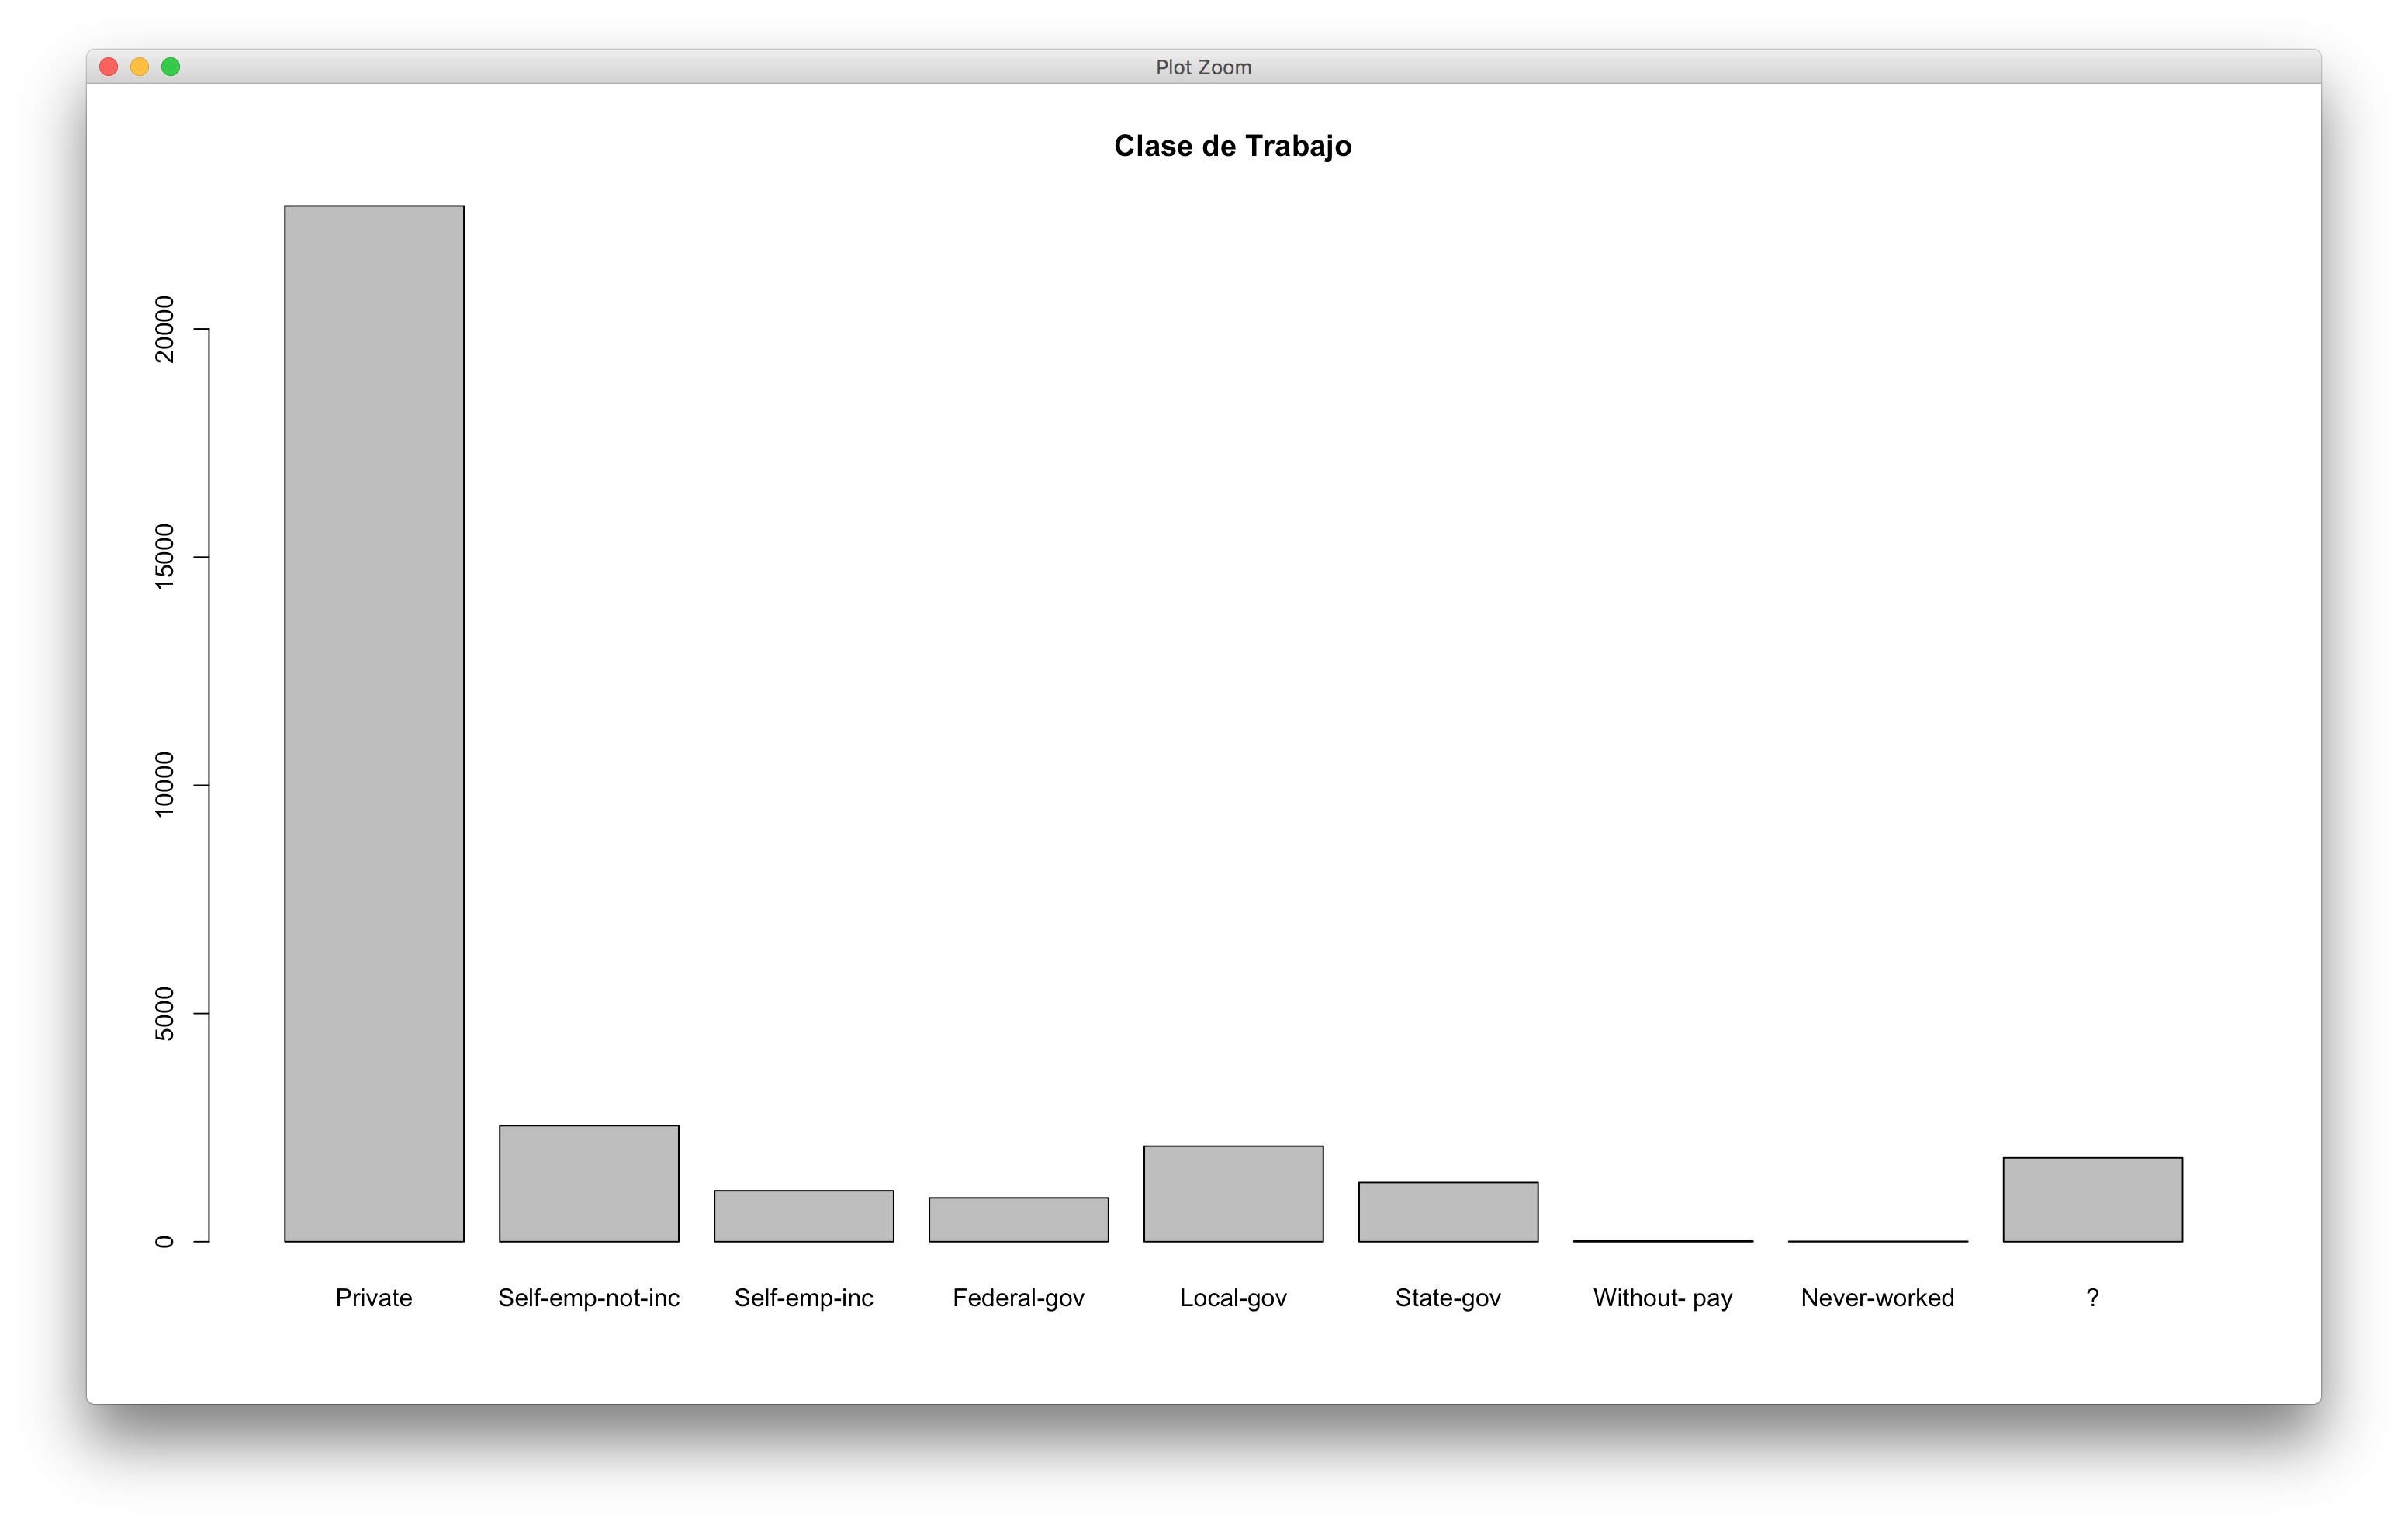
\includegraphics[scale=0.4]{graficas/workclassP}}
  \end{center}
  La mayoría de la gente de nuestro conjunto de datos tiene un trabajo en el sector privado, este tiene una gran diferencia con respecto a los demás, las demás clases de trabajo no rebasan las 4,000 repeticiones, lo cual es demasiado pequeño.
  \begin{center}
    \hbox{\hspace{-5.5em}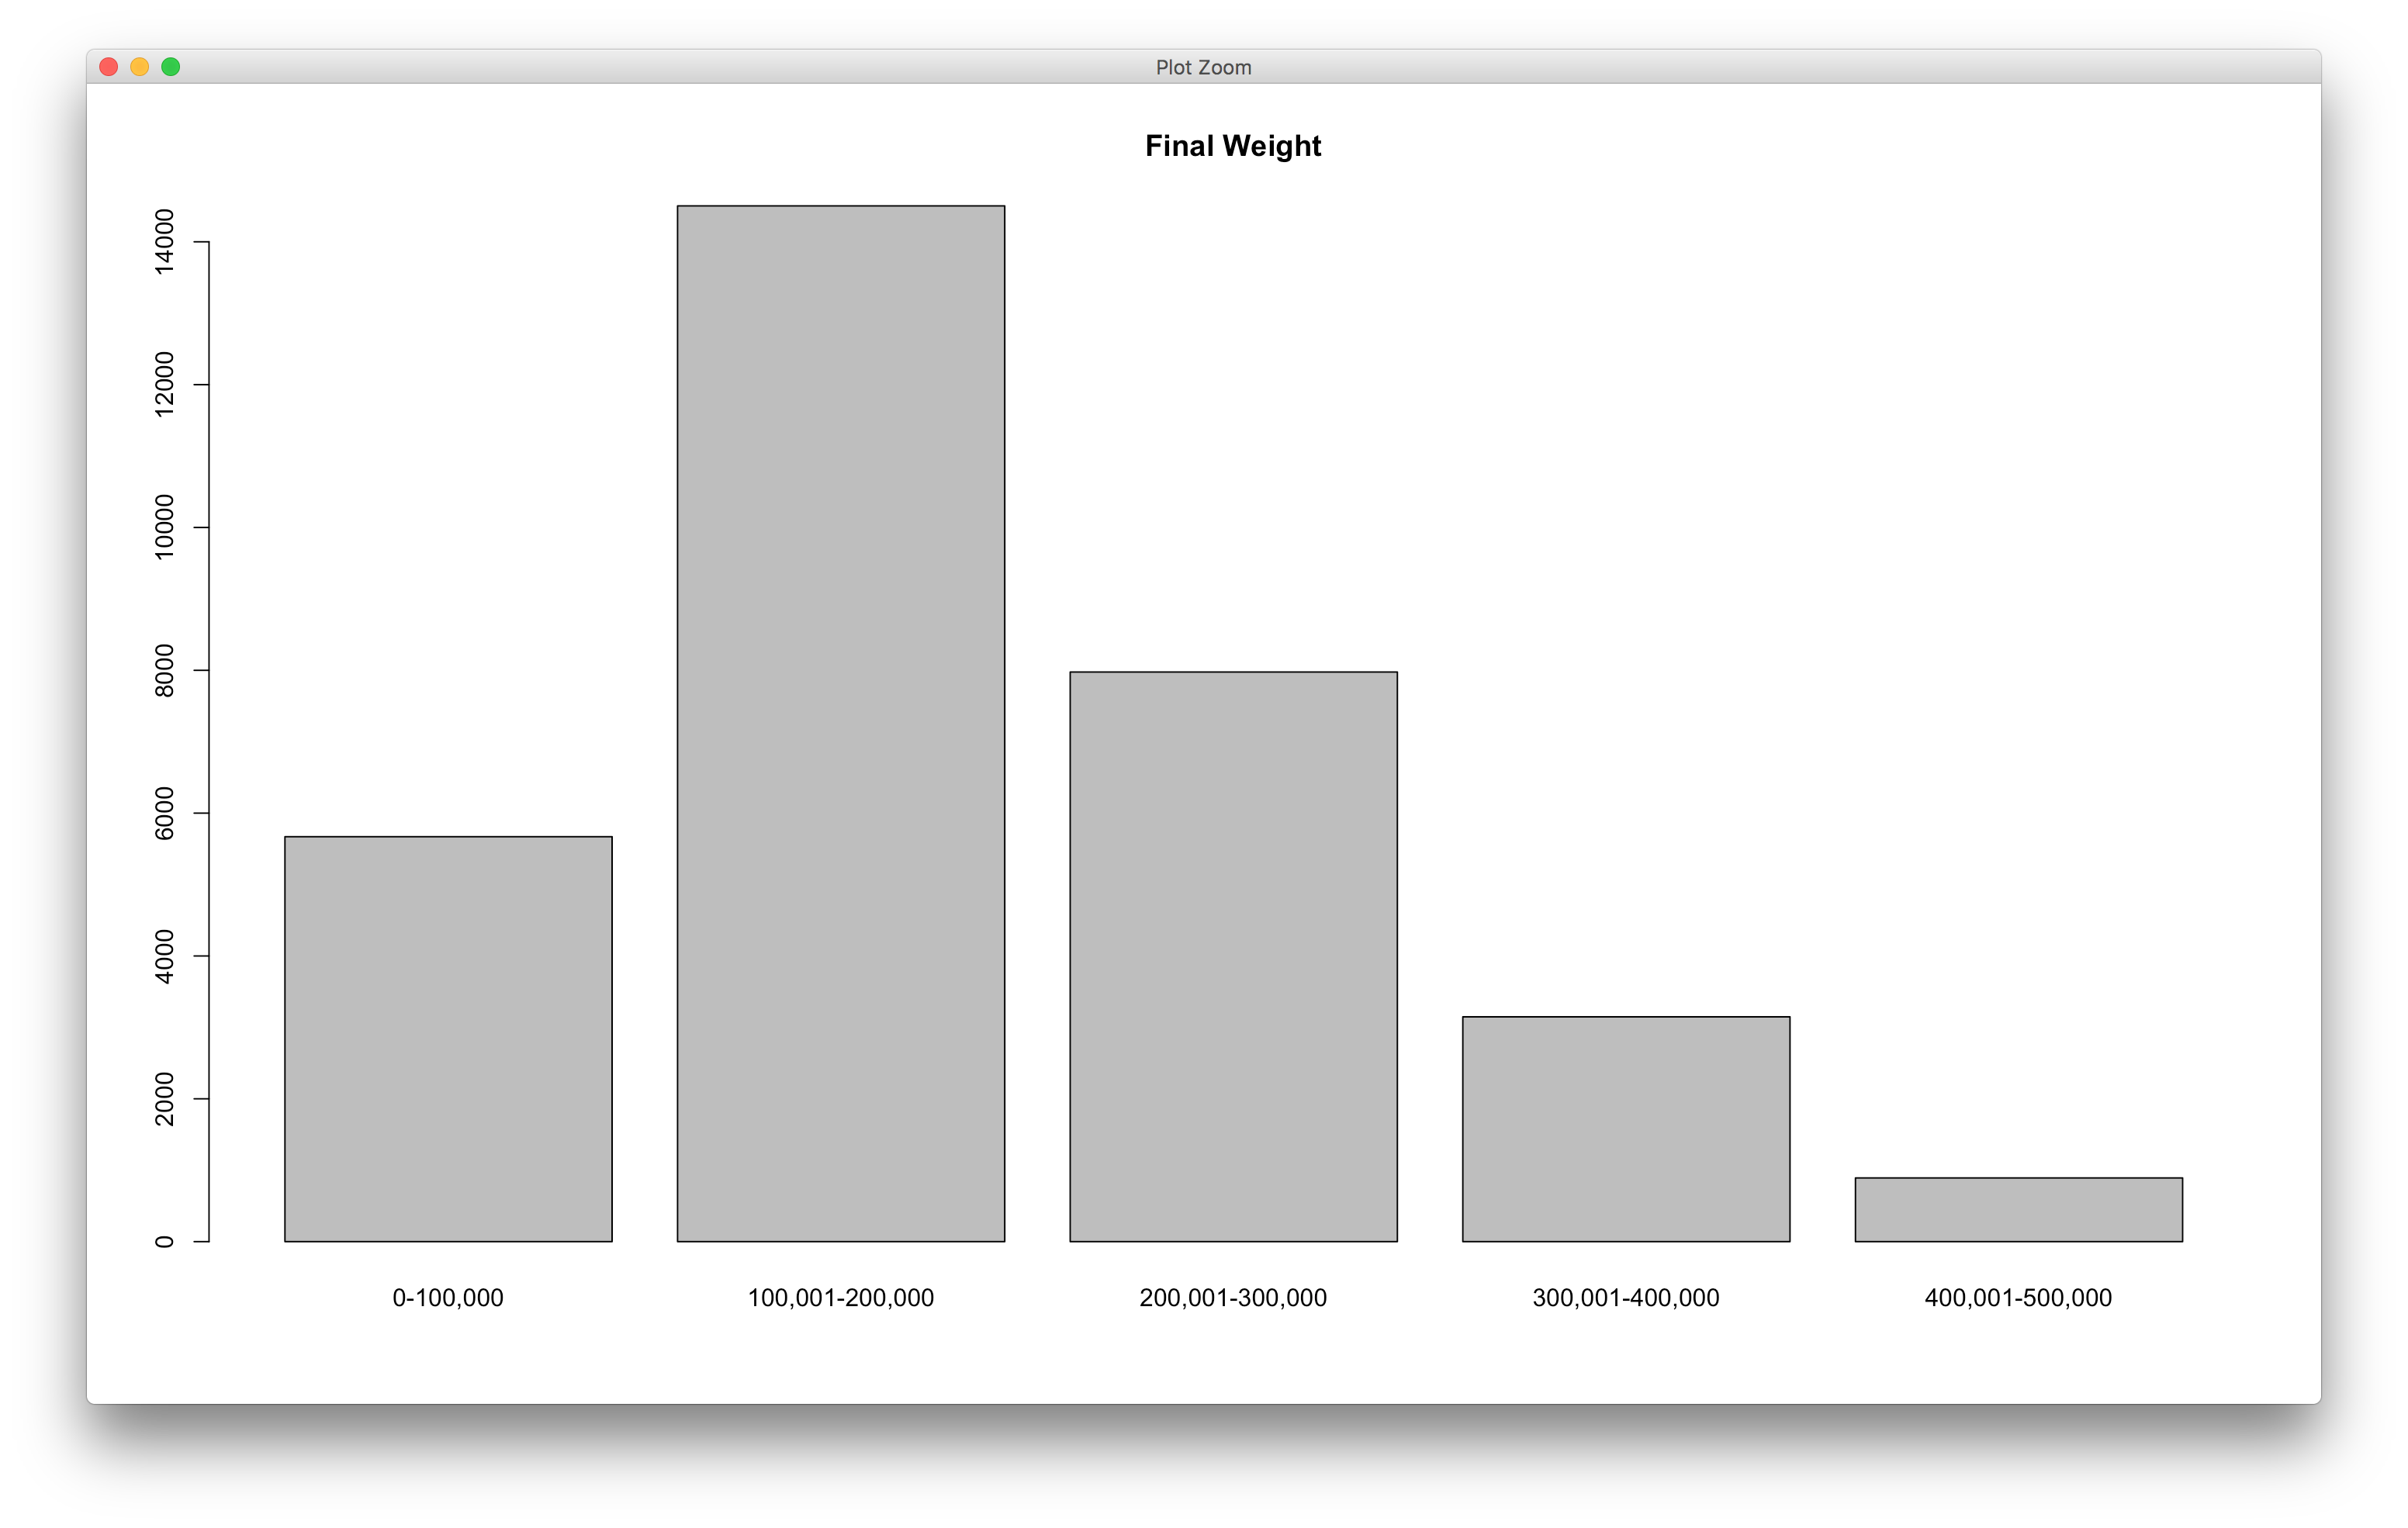
\includegraphics[scale=0.4]{graficas/fnlwgtP}}
  \end{center}
  El rango mas repito es de 100,001 a 200,000, mientras que el menos repetido es el de 400,001, 500,001.
  \begin{center}
    \hbox{\hspace{-5.5em}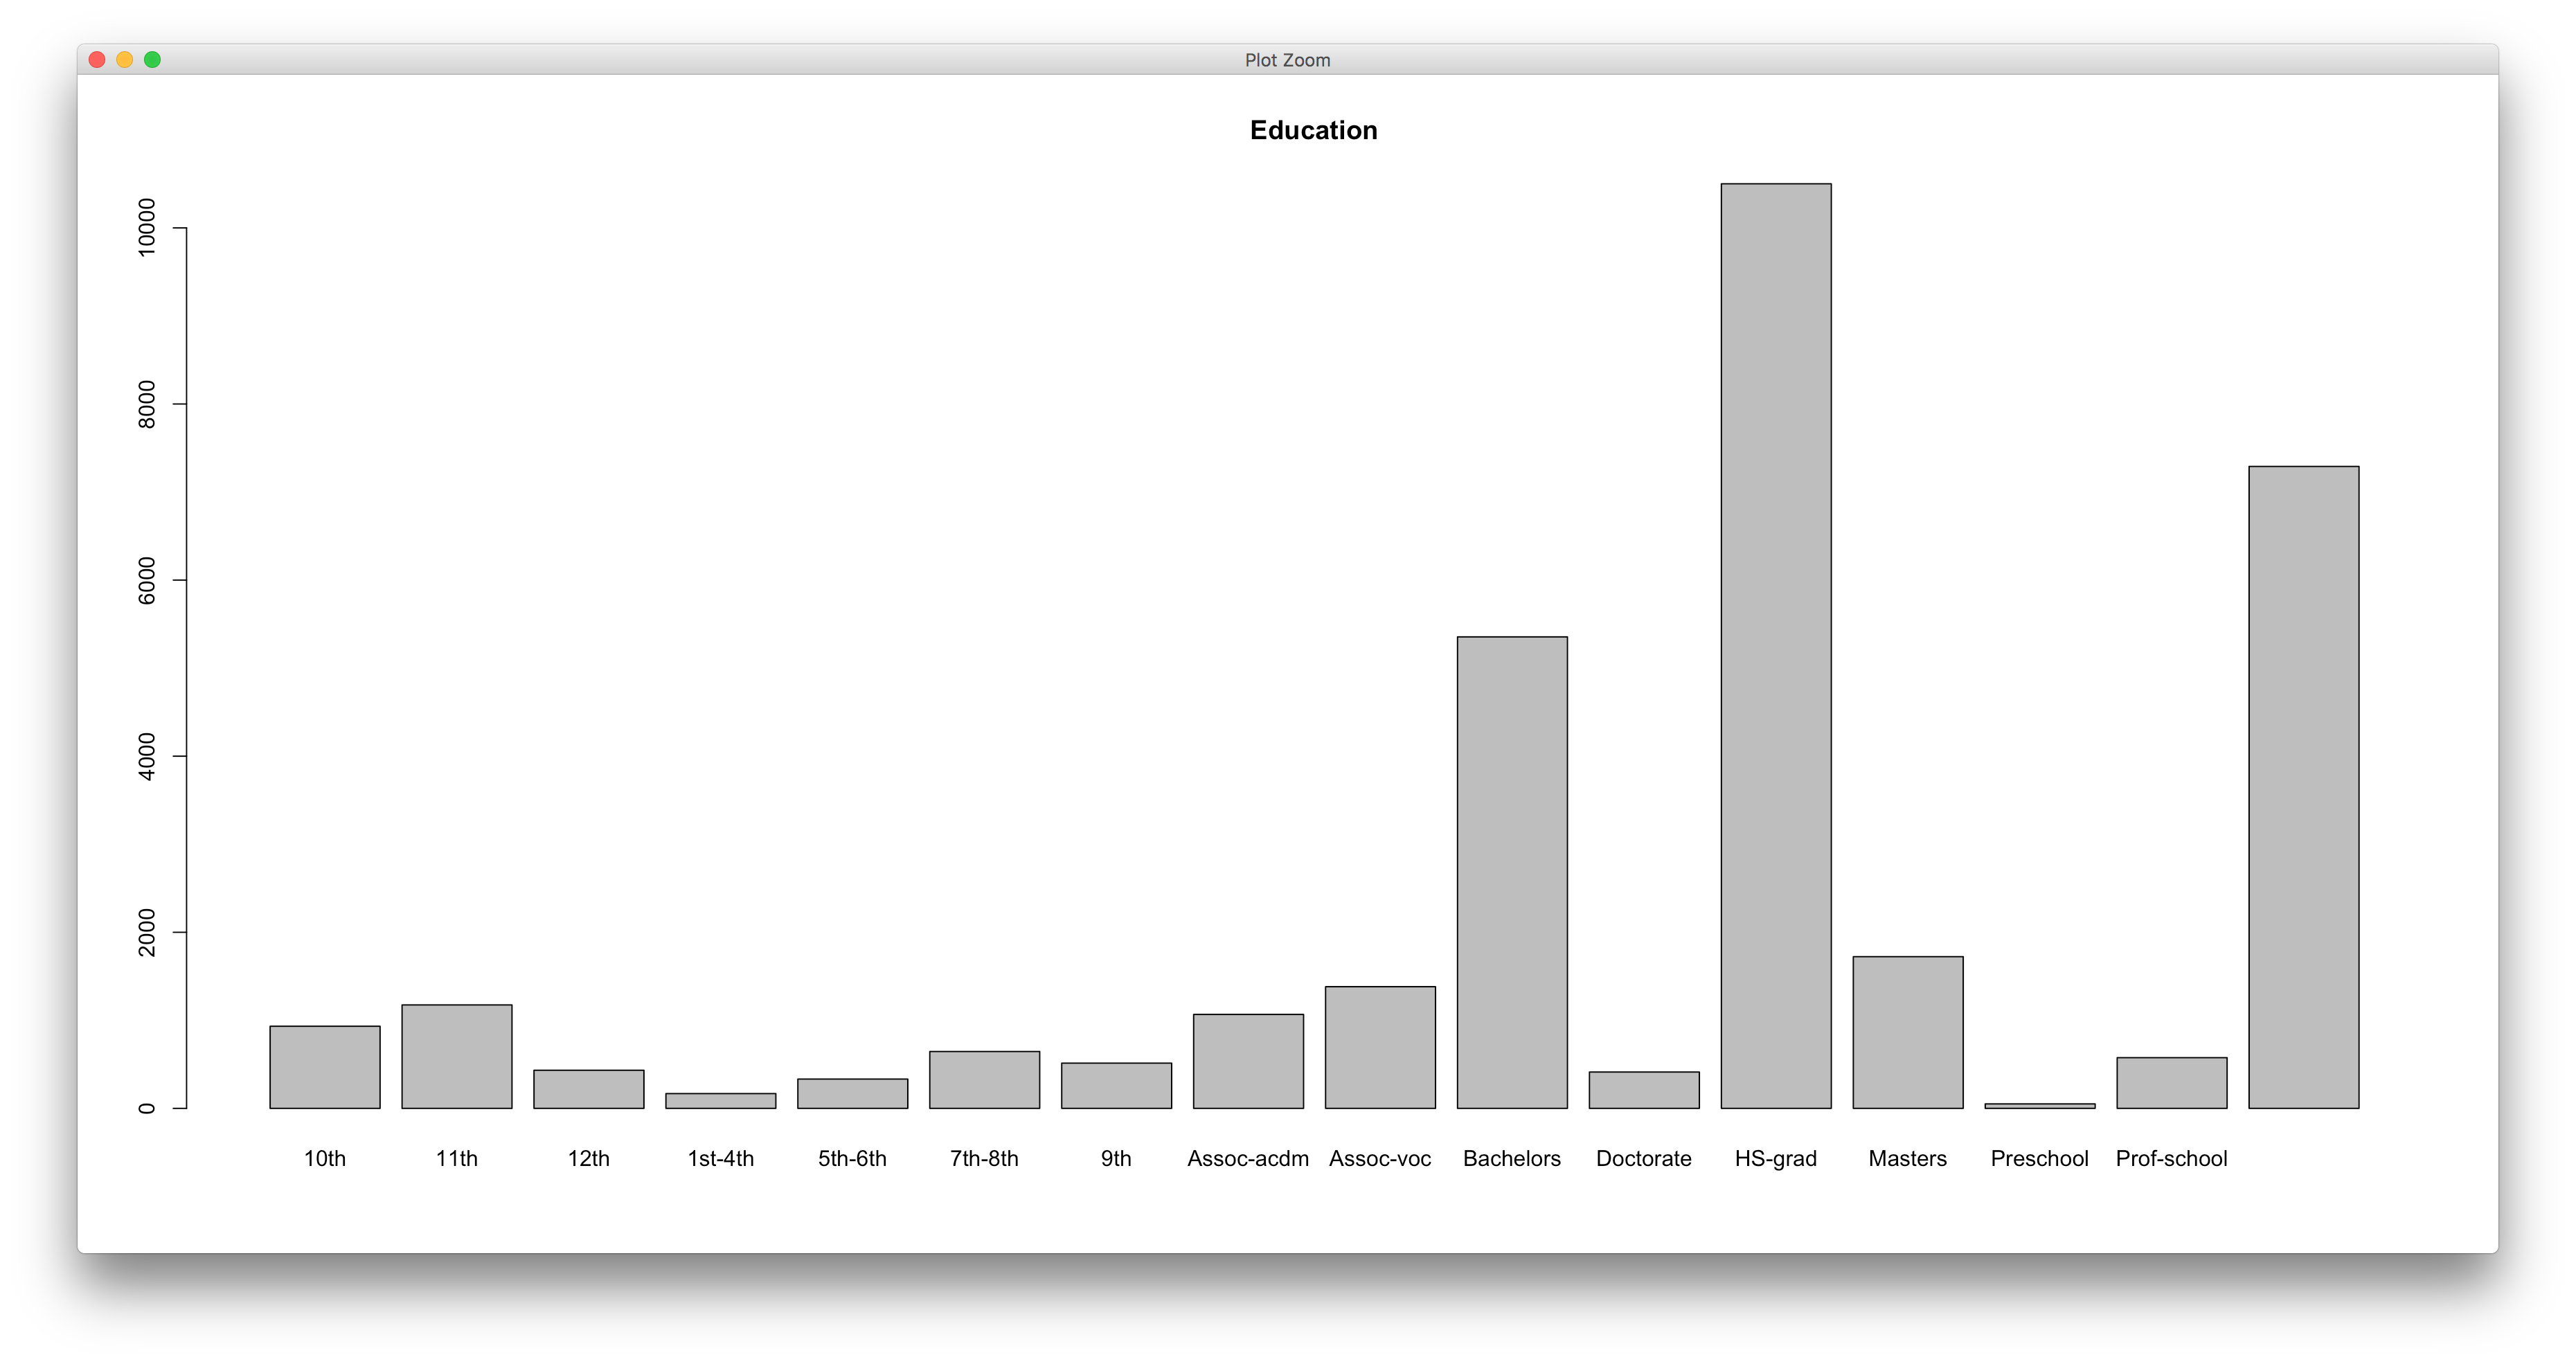
\includegraphics[scale=0.4]{graficas/educationP}}
  \end{center}
  La mayoría de la gente tiene un máximo grado de educación de  preparatoria, el que queda en segundo lugar es grado universitario. Podemos observar que los menores son los que tienen menor grado de estudios van de preescolar a sexto grado. También muy pocos tienen el grado de doctor.
  \begin{center}
    \hbox{\hspace{-5.5em}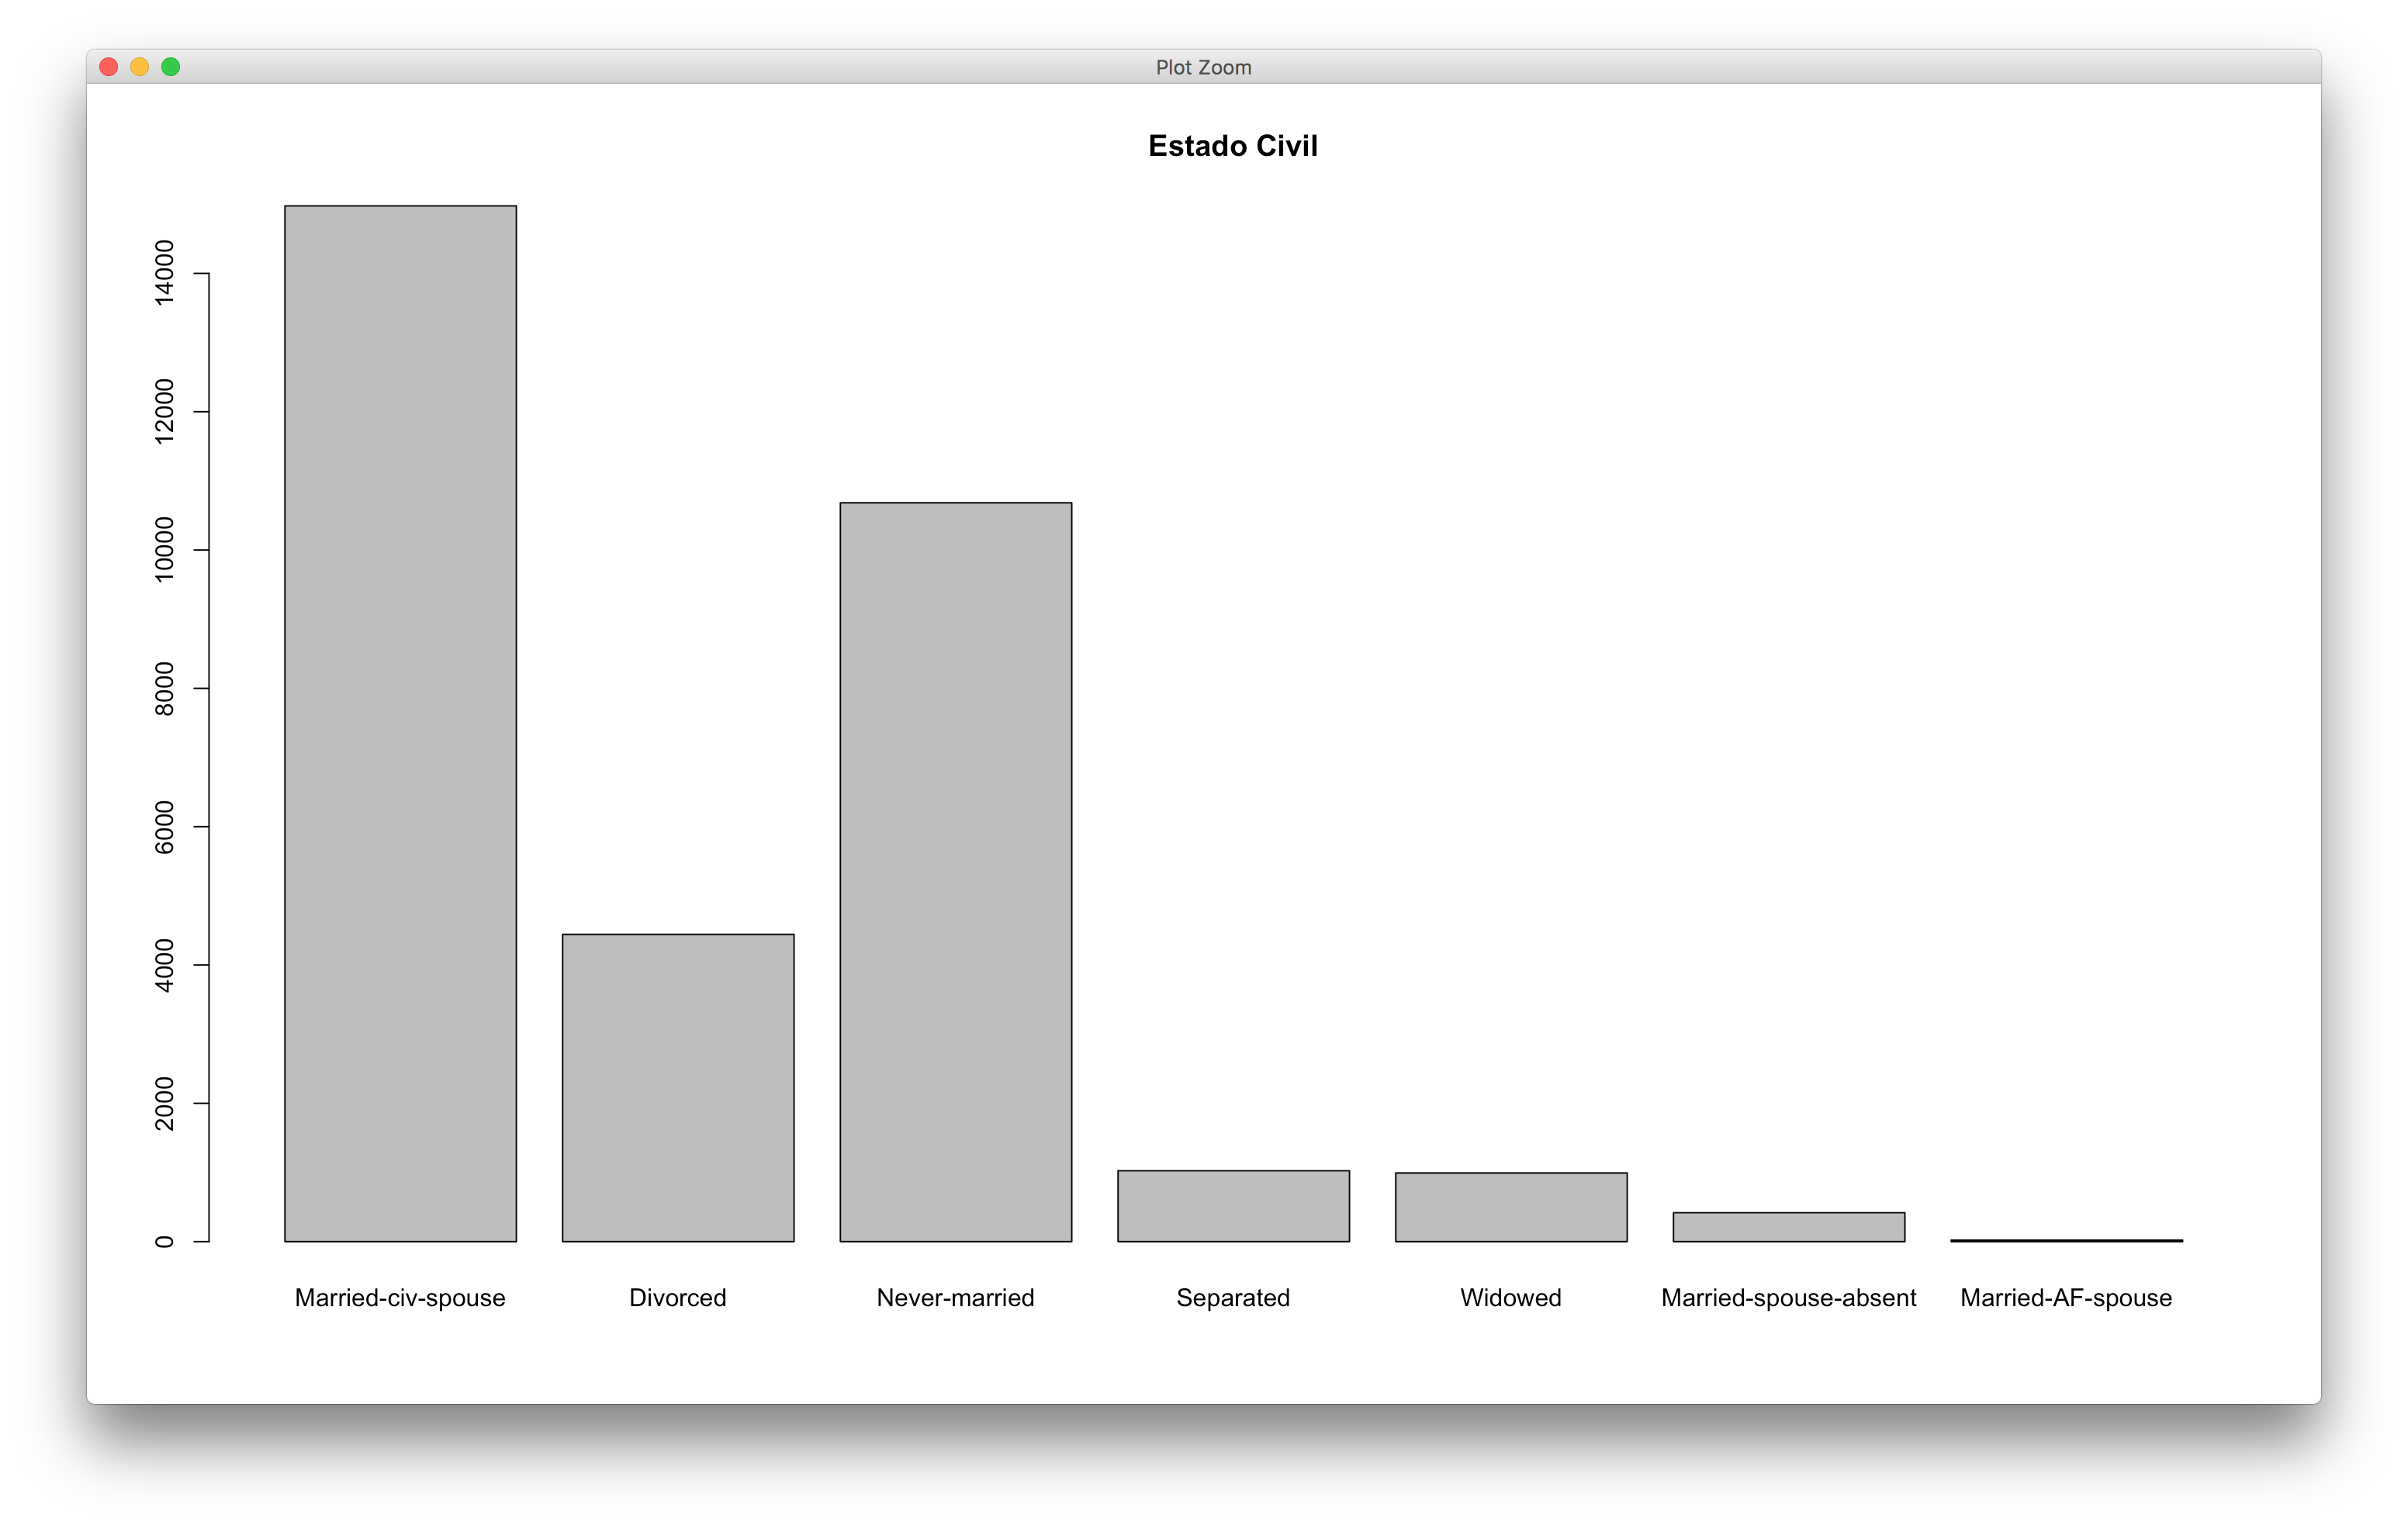
\includegraphics[scale=0.4]{graficas/maritalP}}
  \end{center}
  Mas de la mitad de las personas están casados, mientras que una tercera parte nunca se ha casado. Los estados civiles mas repetidos quedan ordenados de forma descendente de la siguiente manera: casado, nunca casado y divorciado.
  \begin{center}
    \hbox{\hspace{-5.5em}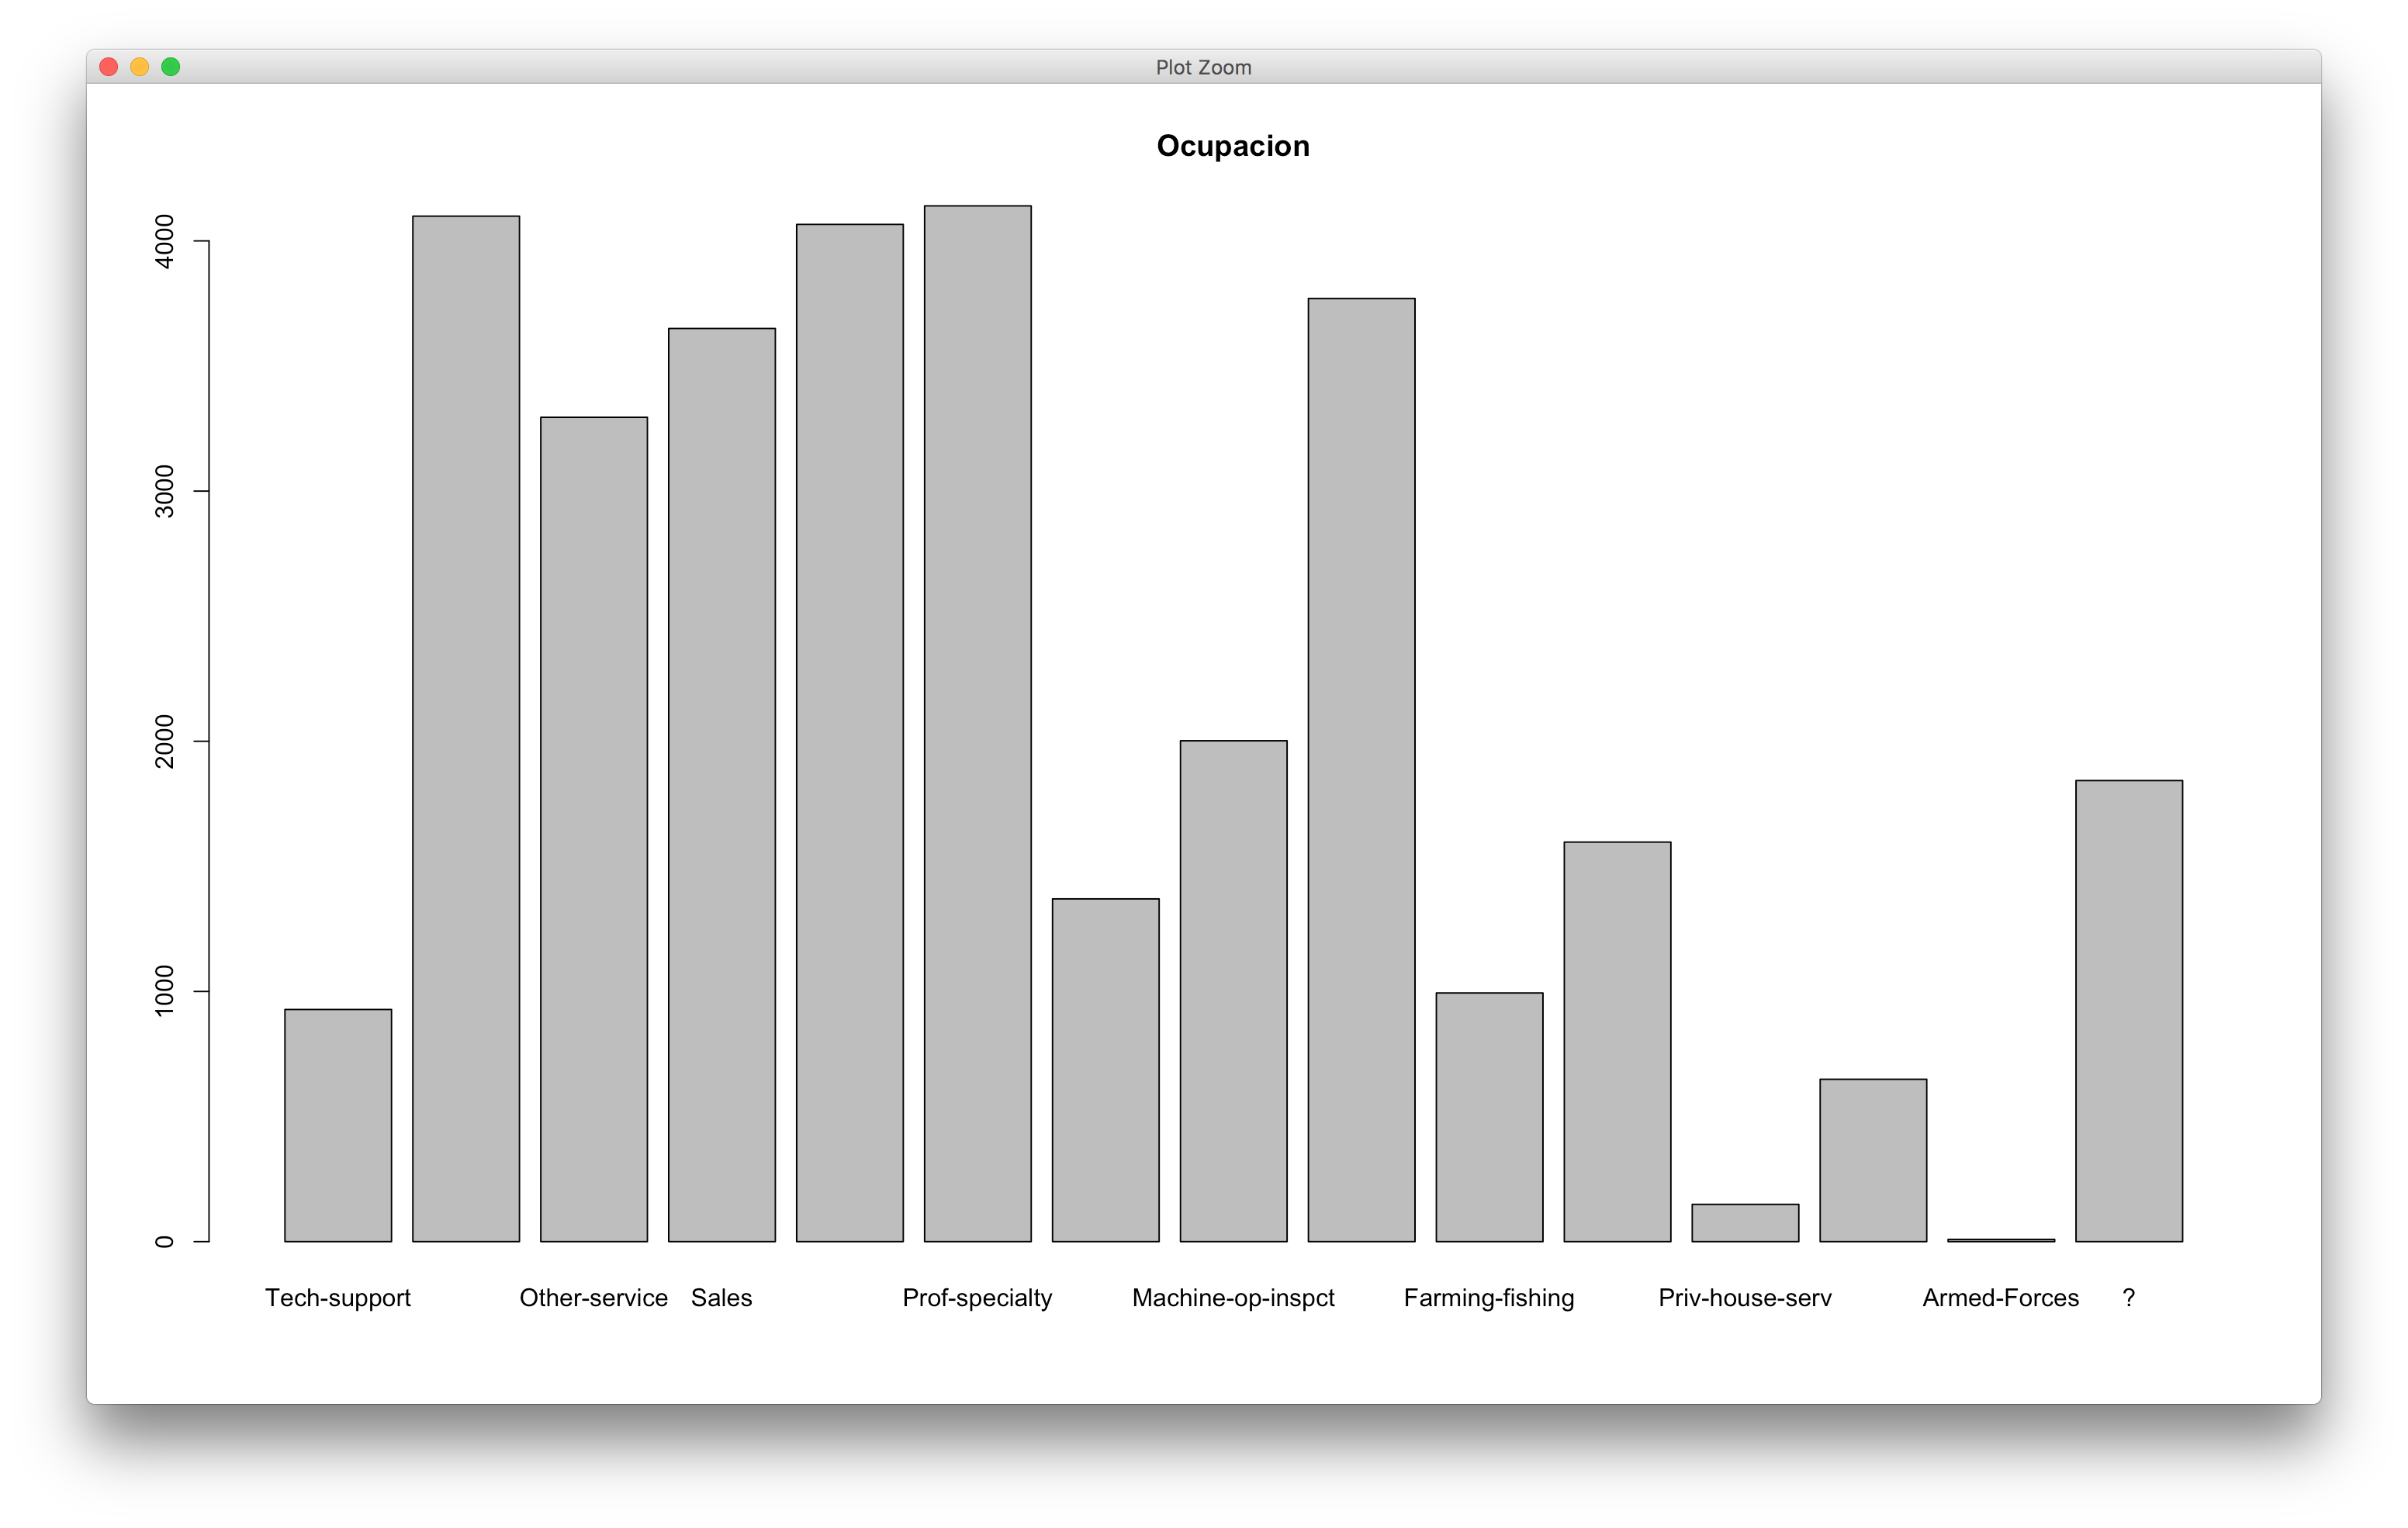
\includegraphics[scale=0.4]{graficas/ocupacionP}}
  \end{center}
  Podemos observar que 6 ocupaciones por lo menos se repiten mas de 3,000 veces, mientras que 9 ocupaciones están por debajo de 2,000. Es importante resaltar que no sabemos la ocupación de 2,000 personas.
  \begin{center}
    \hbox{\hspace{-5.5em}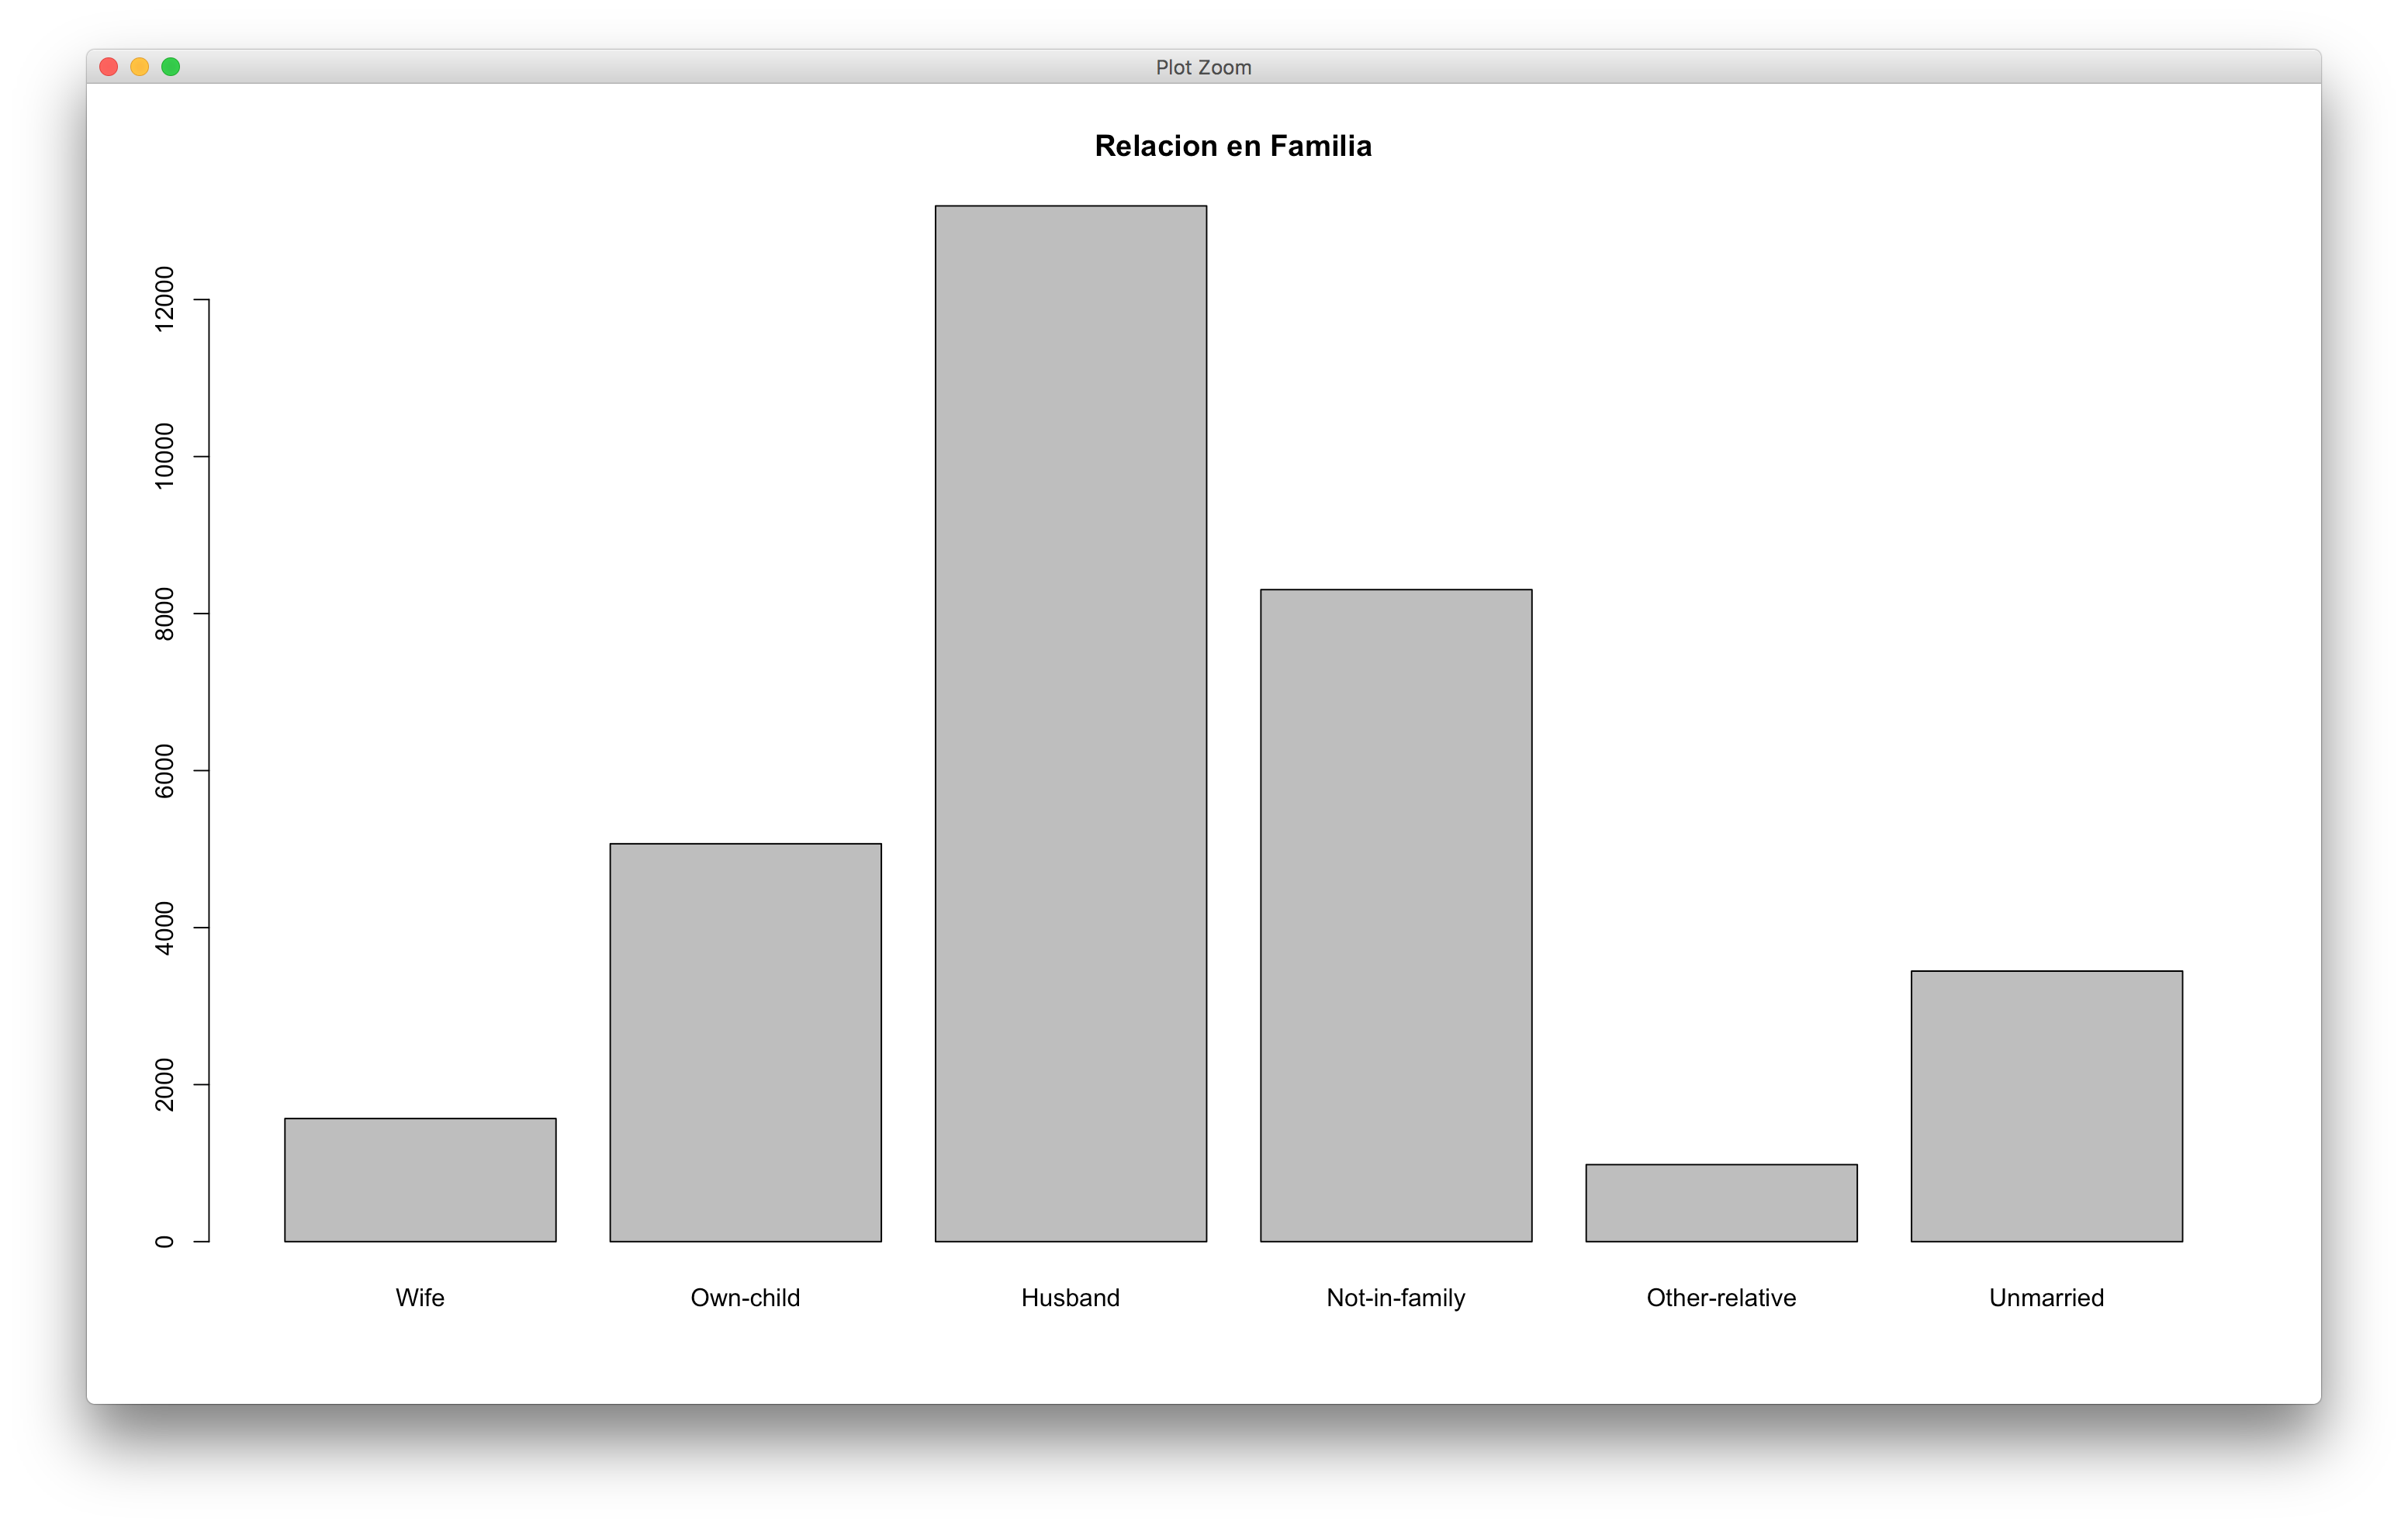
\includegraphics[scale=0.4]{graficas/relfamP}}
  \end{center}
  Mezclando la gráfica de sexo y relación en familia podemos observar que casi la mitad de los hombres juegan el papel de Esposo, mientras que solo una pequeña parte de las mujeres tiene el papel de esposa.
  \begin{center}
    \hbox{\hspace{-5.5em}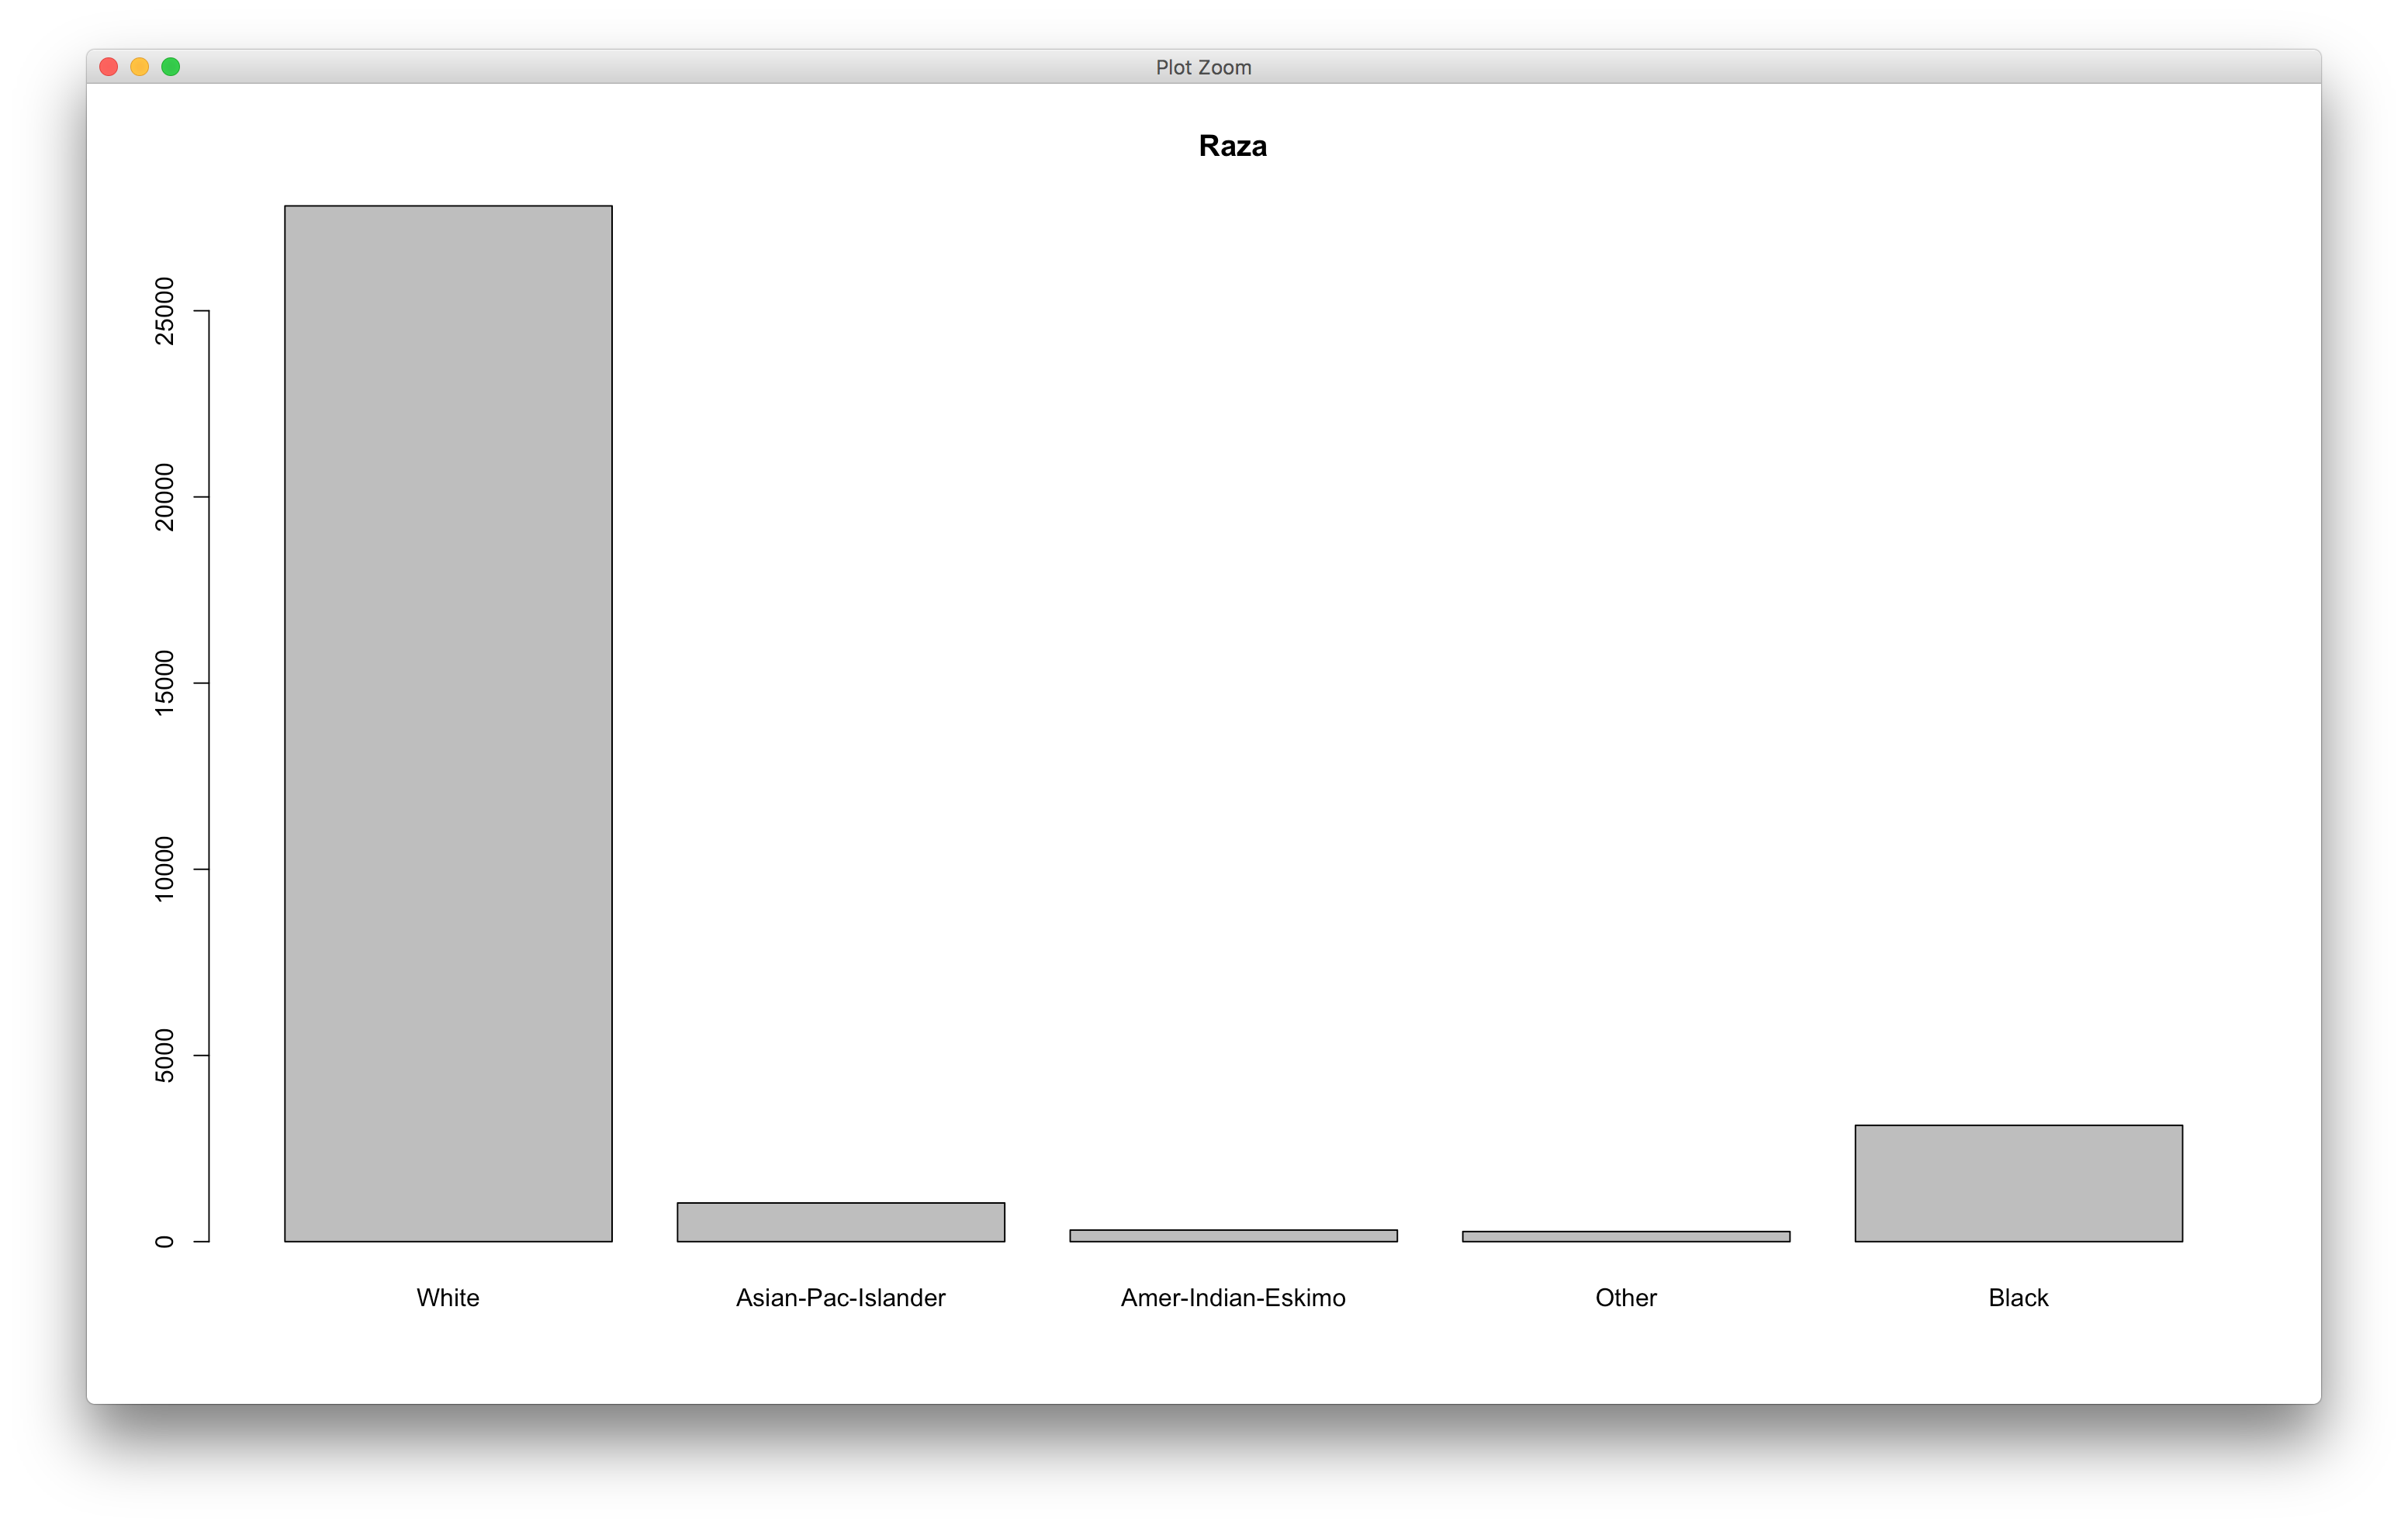
\includegraphics[scale=0.4]{graficas/razaP}}
  \end{center}
  Mas del 70\% de las personas de nuestro conjunto de datos es de raza Blanca.
  \begin{center}
    \hbox{\hspace{-5.5em}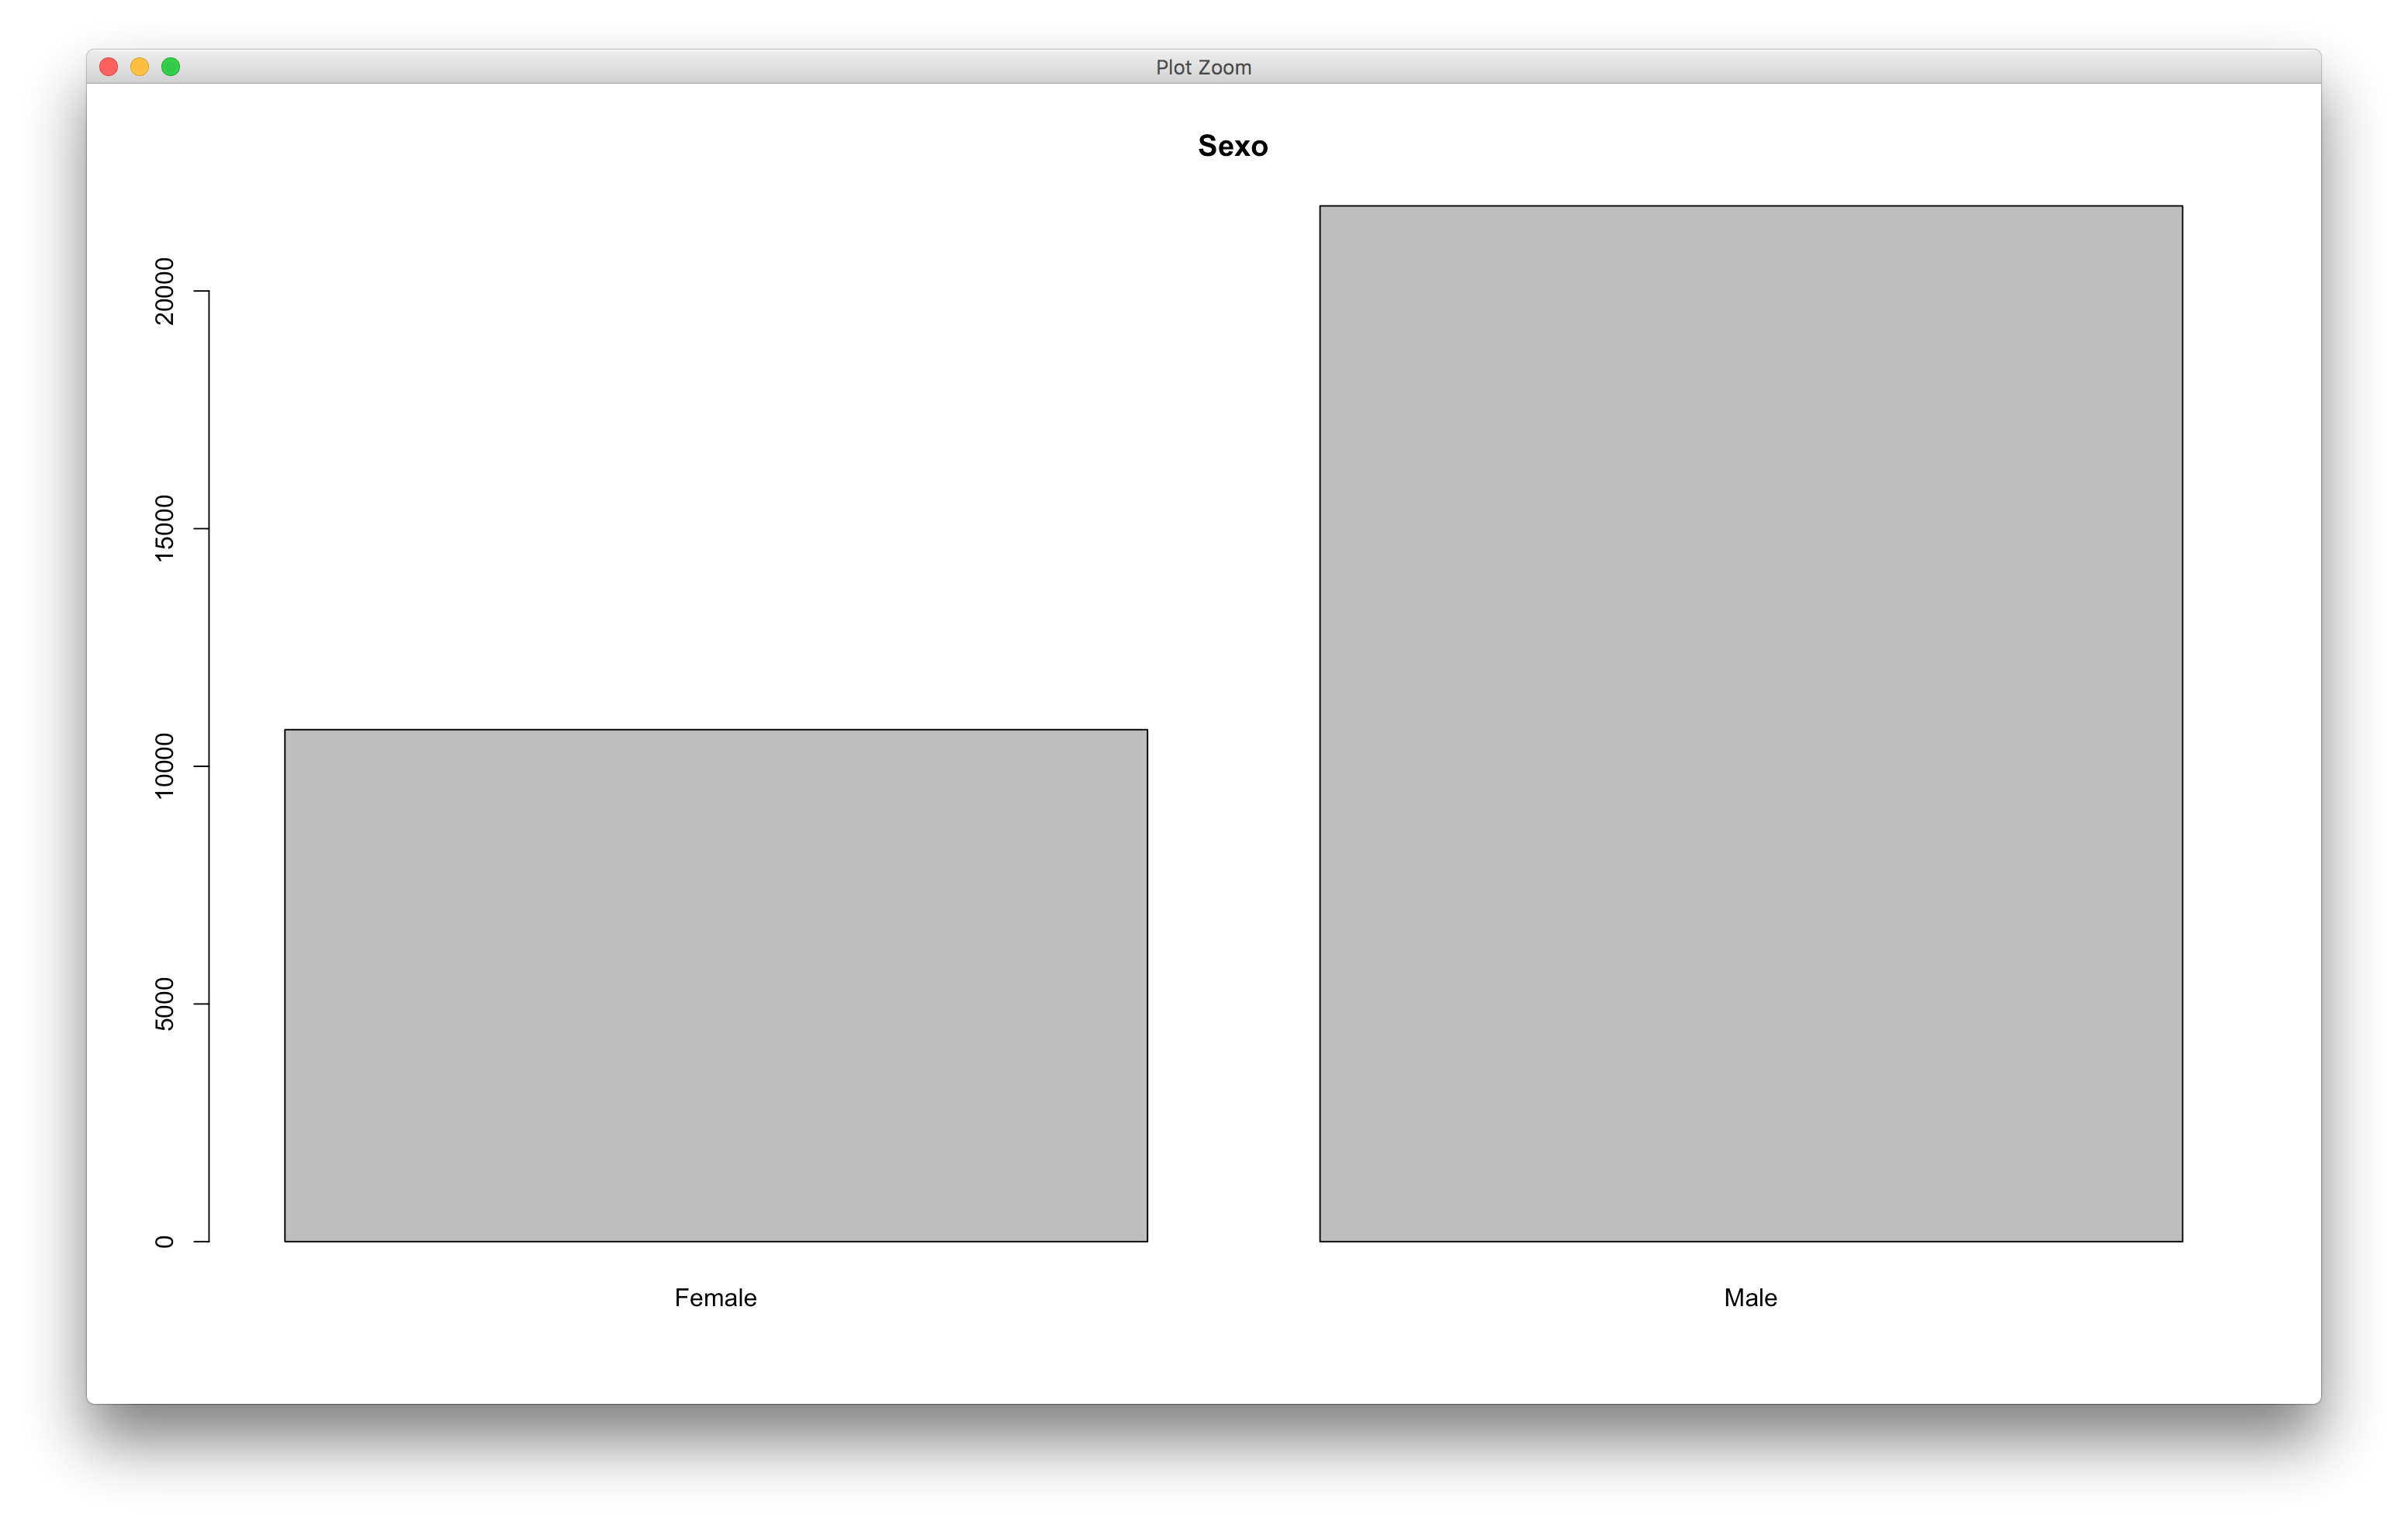
\includegraphics[scale=0.4]{graficas/sexoP}}
  \end{center}
  Mas del 60\% de nuestra población es hombre.
  \begin{center}
    \hbox{\hspace{-5.5em}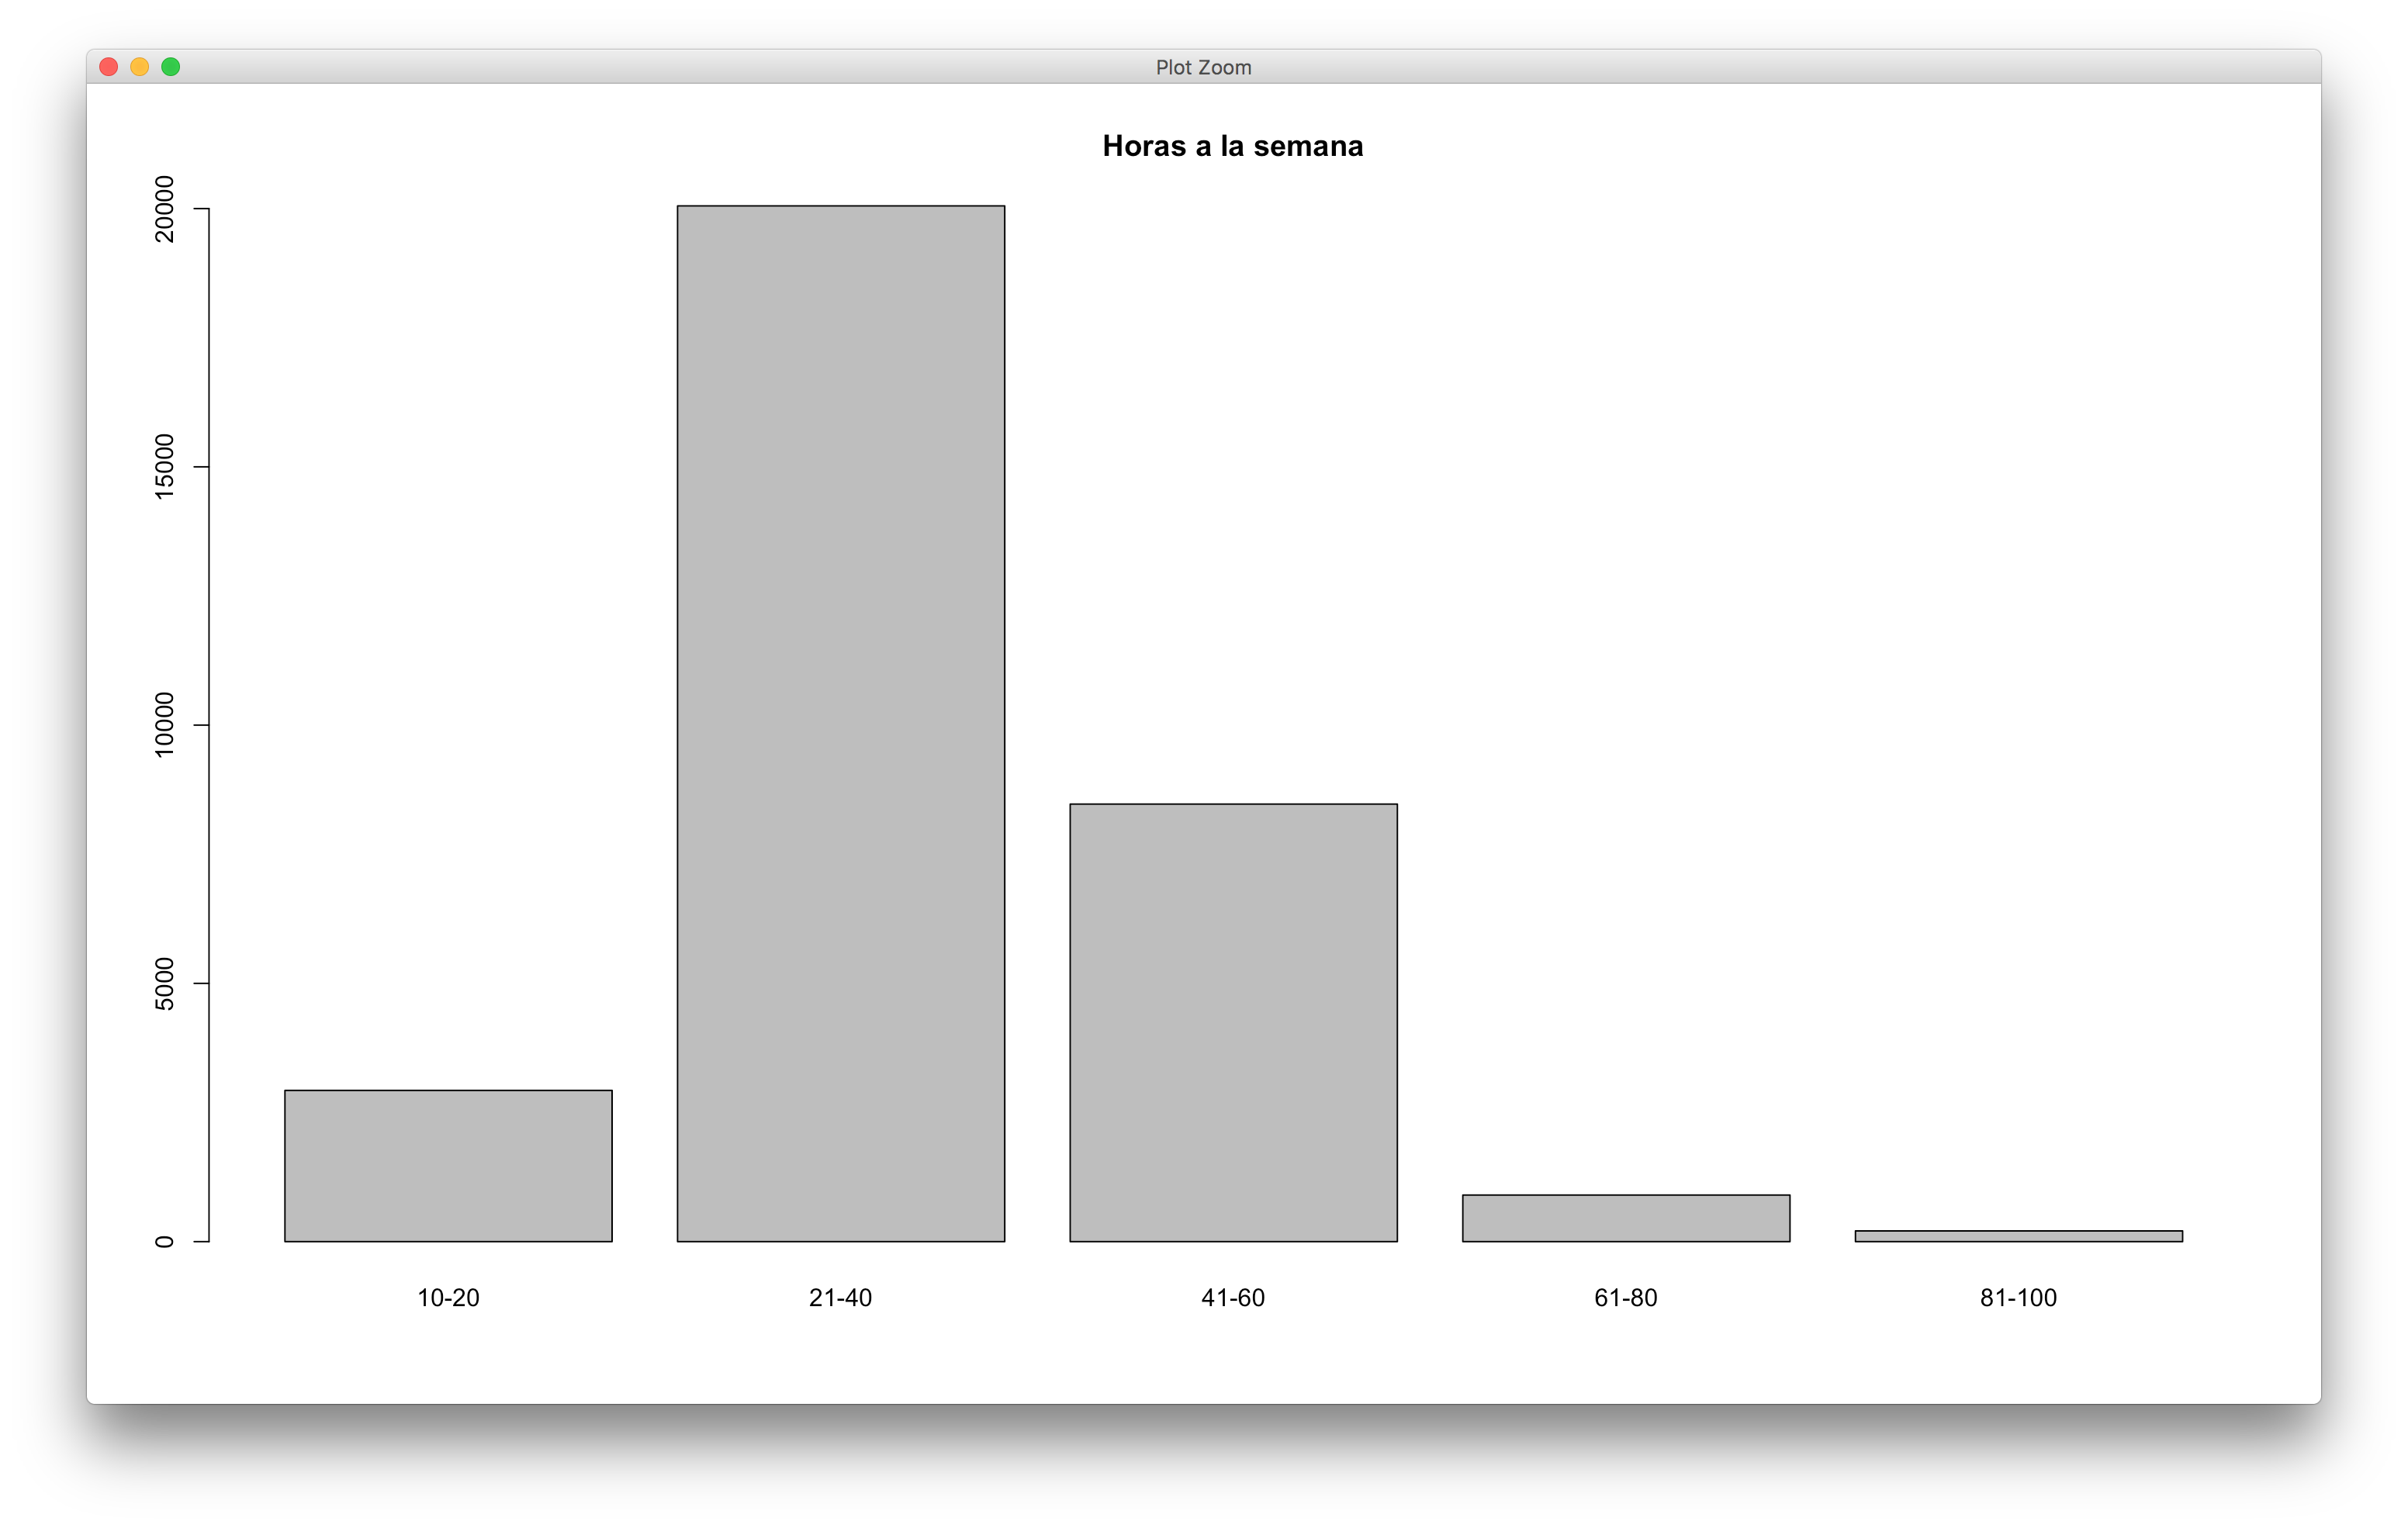
\includegraphics[scale=0.4]{graficas/hpwP}}
  \end{center}
  La mayoría de las personas trabajan entre 21 a 40 horas a la semana.
  \begin{center}
    \hbox{\hspace{-5.5em}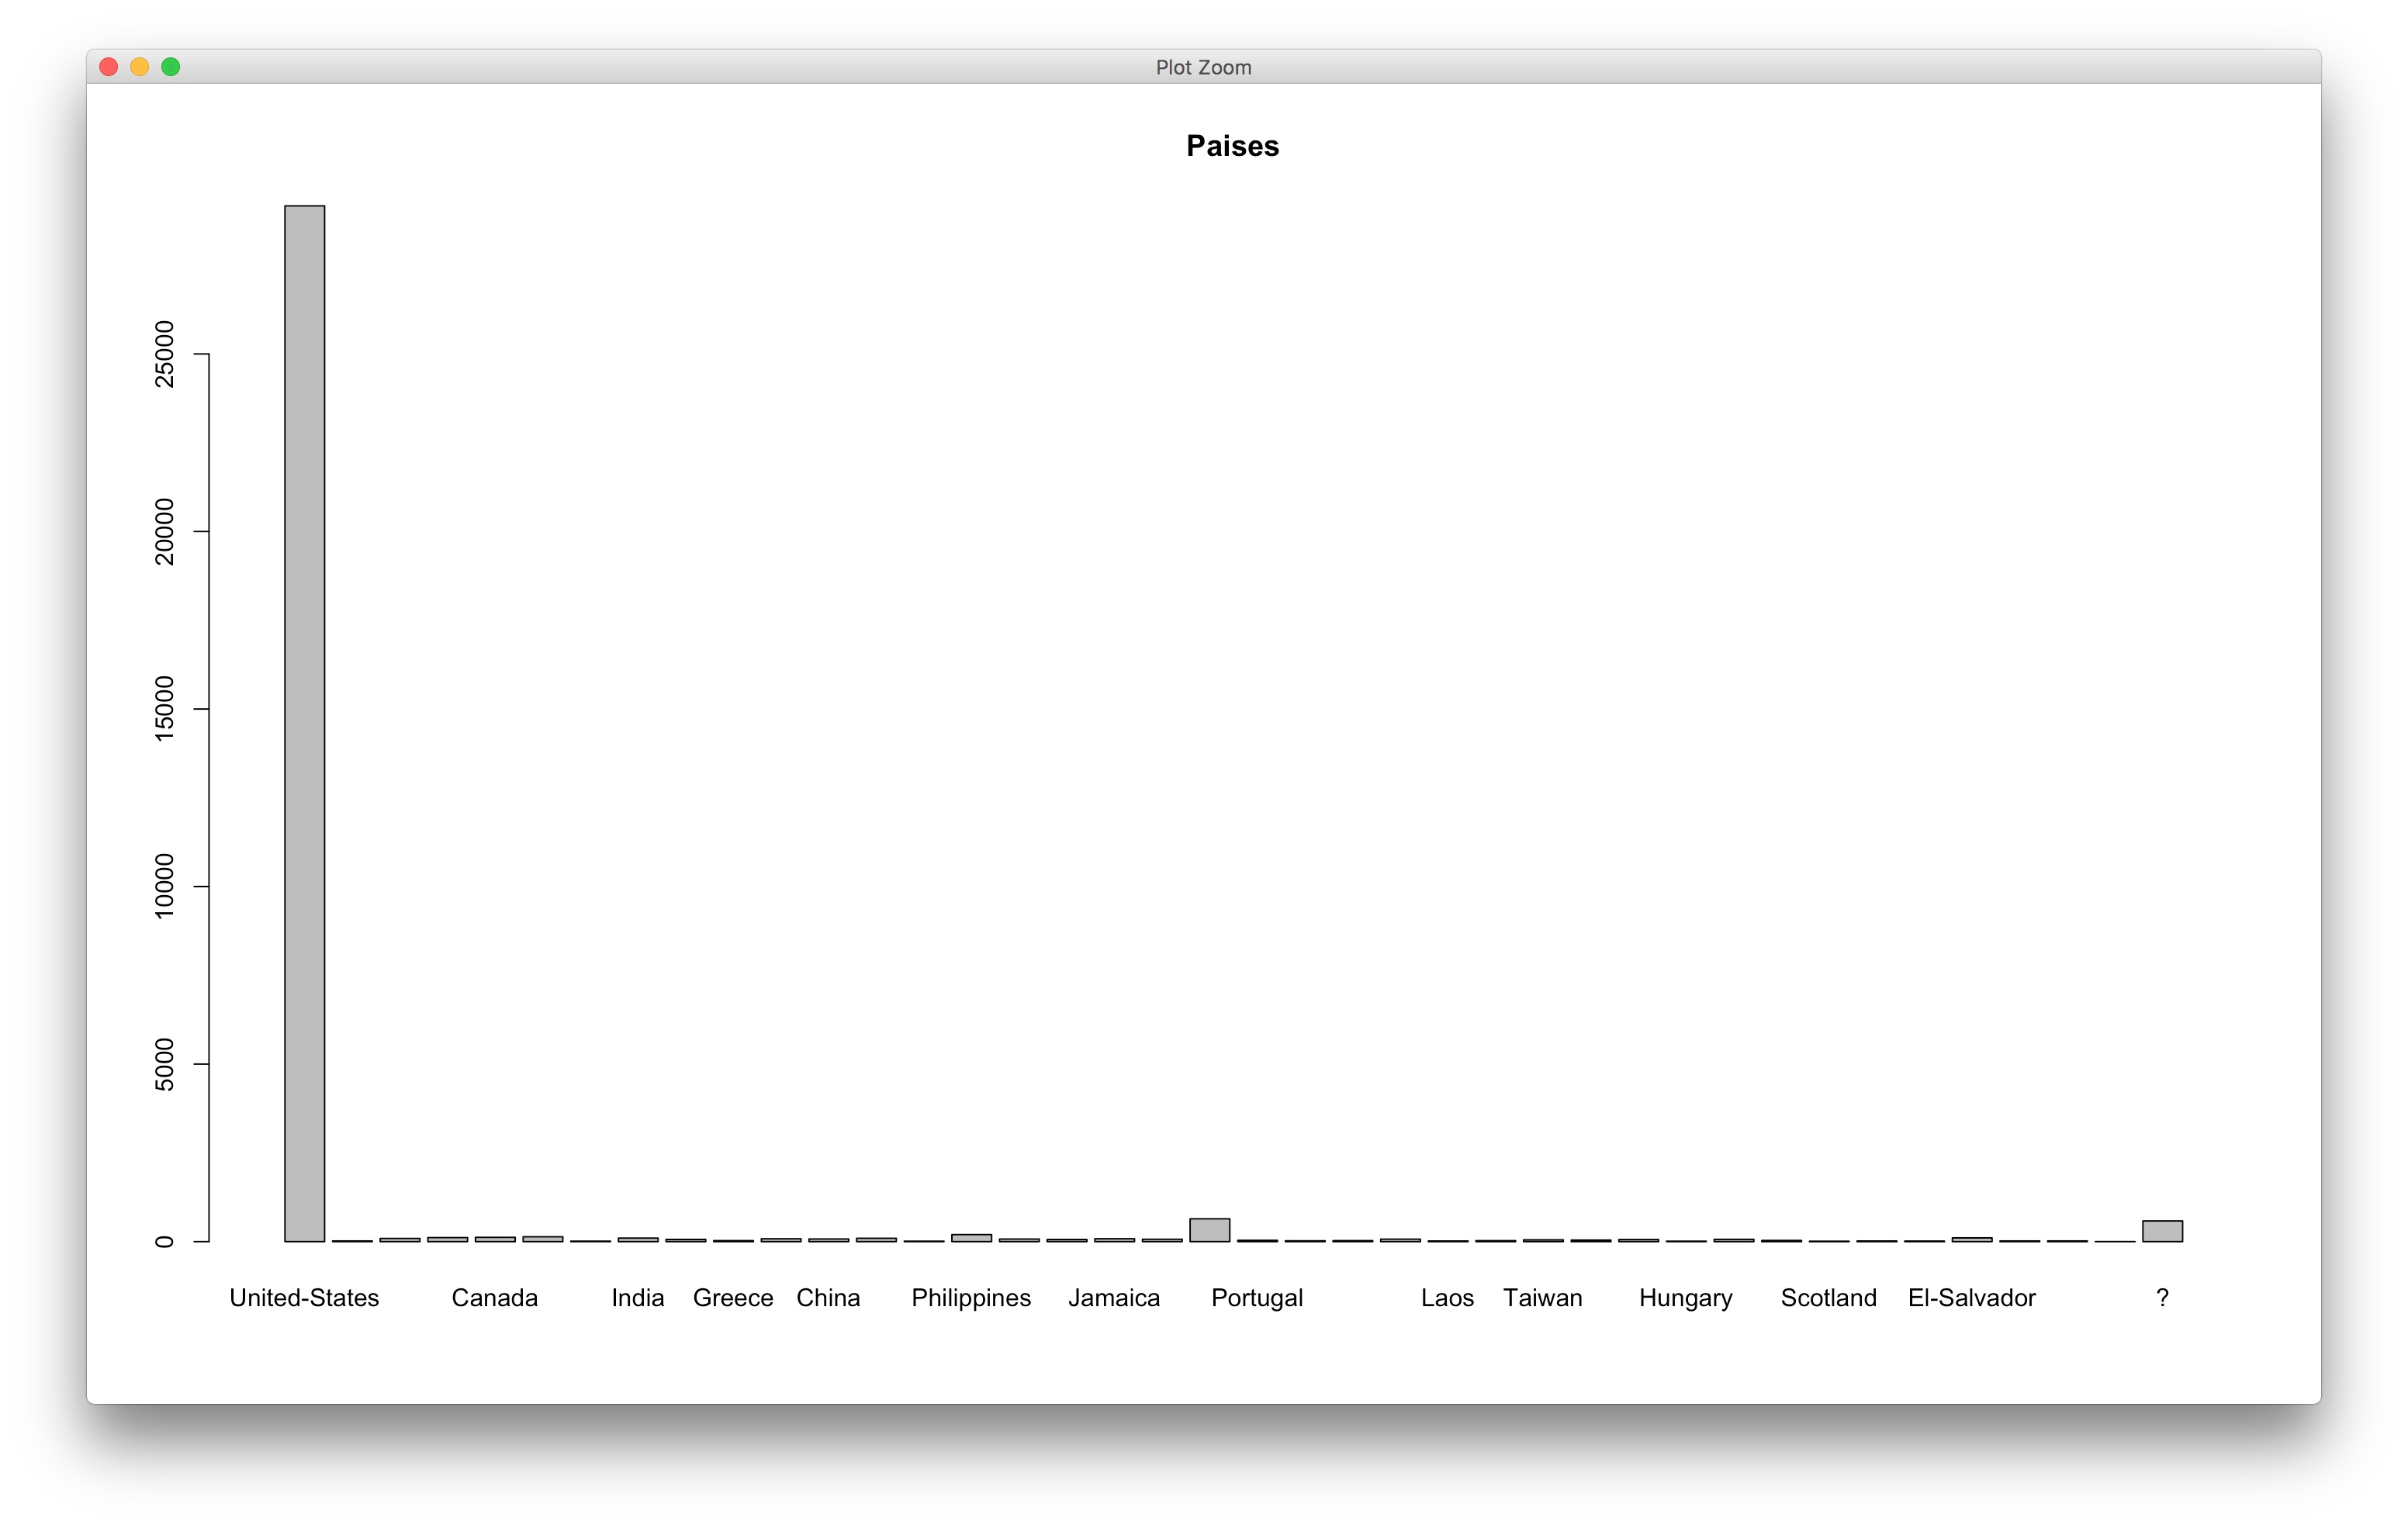
\includegraphics[scale=0.4]{graficas/paisesP}}
  \end{center}
  El país que predomina bastante es estados unidos.
  \begin{center}
    \hbox{\hspace{-5.5em}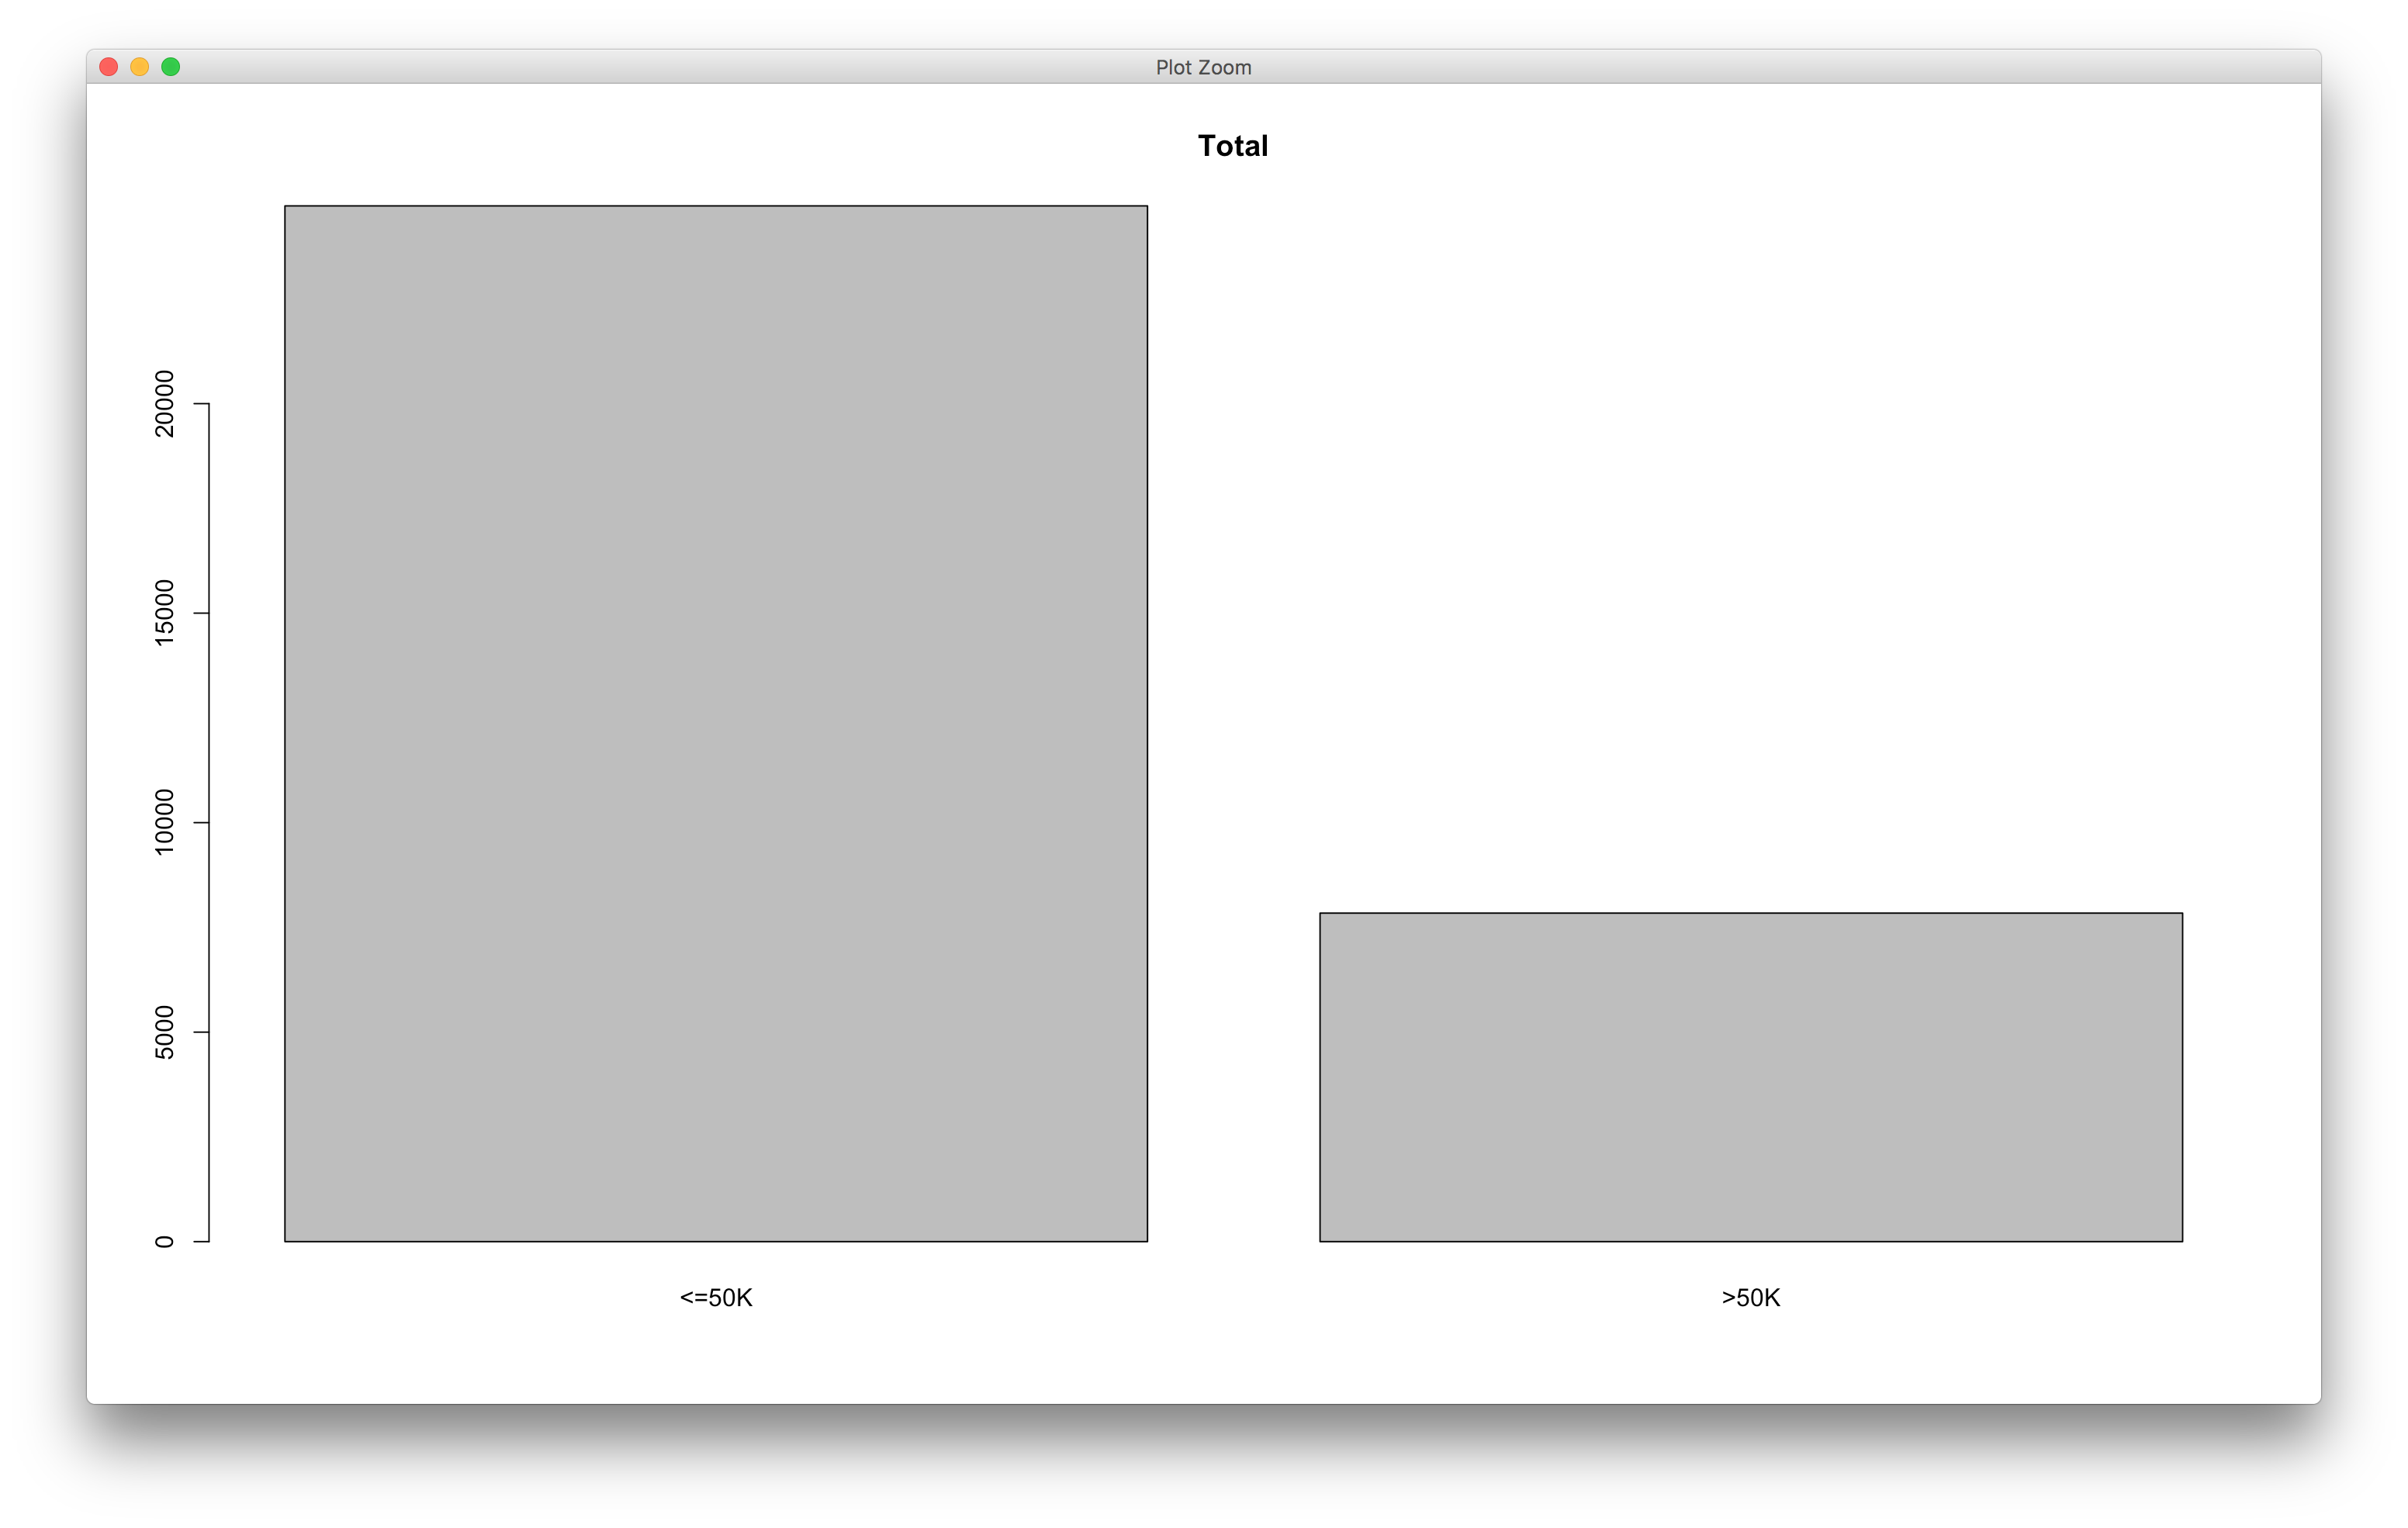
\includegraphics[scale=0.4]{graficas/totalP}}
  \end{center}
  En total mas de la mitad de la gente gana menos de 50k.

\end{document}
